%%%%%%%%%%%%%%%%%%%%%%%%%%%%%%%%%%%%%%%%%%%%%%%%%%%%%%%%%%%%%%%%%%%
%                                                                 %
%                            ROOT FILE                            %
%                                                                 %
%%%%%%%%%%%%%%%%%%%%%%%%%%%%%%%%%%%%%%%%%%%%%%%%%%%%%%%%%%%%%%%%%%%
%
%  Run LaTeX or pdfLaTeX on this file to produce your thesis.
%  To produce the abstract title page followed by the abstract,
%  see the file abstitle-phd.tex or abstitle-mas.tex.
%
%%%%%%%%%%%%%%%%%%%%%%%%%%%%%%%%%%%%%%%%%%%%%%%%%%%%%%%%%%%%%%%%%%%

\documentclass[chap]{thesis}

% Use the first command below if you want captions over 1 line indented. A side
% effect of this is to remove the use of bold for captions (thesis default).
% To restore bold, also include the second line below.
%\usepackage[hang]{caption}      % to indent subsequent lines of captions
%\renewcommand{\captionfont}{\bfseries} % bold caption (needed with caption
                                       % package to restore boldface.)


%\includeonly{rpichap1}  % use \includeonly to process only
                         % the file(s) listed inside the braces


% ------------------------
% You MUST attribute any previously published work (even if it's your own writing)
% Attribution of previously published work
% Use the after title and before the first sentence of the chapter
% Example: \blfootnote{This work perviously appeared as: \bibentry{mypaper2015}
\makeatletter
\def\blfootnote{\xdef\@thefnmark{}\@footnotetext}
\makeatother
\usepackage{graphicx}
\usepackage{adjustbox}
\usepackage{minted}
\usepackage{textcomp}
\usepackage{tabularx}
\usepackage{tikz}
\usetikzlibrary{positioning}
\usepackage{bibentry}
\usepackage{url}
%http://tex.stackexchange.com/questions/141247/how-to-deal-with-sign-in-url-when-using-hyperref-and-bibentry
\usepackage{etoolbox}
\makeatletter
\let\ORIG@BR@c@bibitem\BR@c@bibitem
\apptocmd\ORIG@BR@c@bibitem{\endgroup}{}{}
\def\BR@c@bibitem{\begingroup\catcode`\%=12 \ORIG@BR@c@bibitem}
\makeatother
\nobibliography*

% If you have an attribution before your first in-text citation, 
% you should use \nobibentry to ensure in-text citations start at [1]
\newcommand{\ignore}[1]{}
\newcommand{\nobibentry}[1]{{\let\nocite\ignore\bibentry{#1}}}
% ------------------------

\newcolumntype{L}[1]{>{\raggedright\arraybackslash}p{#1}}
\newcolumntype{C}[1]{>{\centering\arraybackslash}p{#1}}
\newcolumntype{R}[1]{>{\raggedleft\arraybackslash}p{#1}}

%\lstset{
%	basicstyle=\ttfamily,
%	captionpos=b,
%	columns=fullflexible,
%	frame=single,
%	breaklines=true,
%	numbers=left,
%	numbersep=5pt,
%}

\begin{document}

%\include{rpititle-mas}   % titlepage material for Master's thesis or project
%%%%%%%%%%%%%%%%%%%%%%%%%%%%%%%%%%%%%%%%%%%%%%%%%%%%%%%%%%%%%%%%%%%
%                                                                 %
%                            TITLE PAGE                           %
%                            PhD Thesis                           %
%                                                                 %
%%%%%%%%%%%%%%%%%%%%%%%%%%%%%%%%%%%%%%%%%%%%%%%%%%%%%%%%%%%%%%%%%%%
%  This file produces the title page, copyright page (if requested)
%  and the Table of Contents, List of Figures and List of Tables.
%
%  To produce the abstract title page followed by the abstract,
%  see the template file, "abstitle-phd.tex"
%%%%%%%%%%%%%%%%%%%%%%%%%%%%%%%%%%%%%%%%%%%%%%%%%%%%%%%%%%%%%%%%%%%

% Supply information for use on title page:
%
\thesistitle{\bf Dataset Versioning through \\ Linked Data Models}
\author{Benno Lee}
\degree{Doctor of Philosophy}
\department{Computer Science} % provide your area of study here; e.g.,
%  "Mechanical Engineering", "Nuclear Engineering", "Physics", etc.

\signaturelines{4}     %max number of signature lines is 7
\thadviser{Peter Fox}
 %\cothadviser{Second Adviser} % If you have 2 thesis advisers
\memberone{Jim Hendler}
\membertwo{Deborah MacGuiness}
\memberthree{Beth Plale}
%\memberfour{Marcus Aurelius} % must change signaturelines to 5 if using this 5 members
%\memberfive{Marcus Junius Brutus} % must change signaturelines to 6 if using this 6 members
%\membersix{Nikola Tesla} % must change signaturelines to 7 if using this 7 members

\submitdate{May 2018\\(For Graduation July 2018)}
\copyrightyear{2018}   % if omitted, current year is used.

% Print titlepage and other prefatory material:
%
\titlepage
\copyrightpage         % optional
\tableofcontents
\listoftables          % required if there are tables
\listoffigures         % required if there are figures
\listoflistings   % titlepage material for PhD thesis
%%%%%%%%%%%%%%%%%%%%%%%%%%%%%%%%%%%%%%%%%%%%%%%%%%%%%%%%%%%%%%%%%%%
%                                                                 %
%                         ACKNOWLEDGEMENT                         %
%                                                                 %
%%%%%%%%%%%%%%%%%%%%%%%%%%%%%%%%%%%%%%%%%%%%%%%%%%%%%%%%%%%%%%%%%%%

\specialhead{ACKNOWLEDGMENT}

I would like to thank my committee for their input into my research journey.
I would like to thank Peter Fox for his guidance and advice.
I would like to thank Kathy Fontaine for her guidance and time in editing this document.
I would like to thank my lab mates for insightful and lengthy discussions.  % include for acknowledgements
%%%%%%%%%%%%%%%%%%%%%%%%%%%%%%%%%%%%%%%%%%%%%%%%%%%%%%%%%%%%%%%%%%%
%                                                                 %
%                            ABSTRACT                             %
%                                                                 %
%%%%%%%%%%%%%%%%%%%%%%%%%%%%%%%%%%%%%%%%%%%%%%%%%%%%%%%%%%%%%%%%%%%

\specialhead{ABSTRACT}

Science is constantly changing and the data that drives it changes along with it.
Understanding the behavior of data as it changes to correct errors and to add value, improves data quality and eases data integration.
Current methods to track the evolution of data primarily focus on the collection of data provenance, but lacks the fidelity to evaluate the extent of a change.
The conceptual model proposed in this document addresses this challenge by leveraging semantic technologies to automatically embed versioning information into changelog artifacts generated when changes are made to a dataset.
A method to calculate change distance then follows using the resulting semantic graph by attaching weights to different change types.
Initial applications begin with spreadsheets then databases with the ultimate goal in applying the model to online ontologies. % abstract
%%%%%%%%%%%%%%%%%%%%%%%%%%%%%%%%%%%%%%%%%%%%%%%%%%%%%%%%%%%%%%%%%%%
%                                                                 %
%                            CHAPTER ONE                          %
%                                                                 %
%%%%%%%%%%%%%%%%%%%%%%%%%%%%%%%%%%%%%%%%%%%%%%%%%%%%%%%%%%%%%%%%%%%

\chapter{INTRODUCTION}

Consider the example... --> Bugzilla.
Requirements for Development of Hypermedia Technology for a Digital Library Supporting Scholarly Work \cite{Wiil:2000:RDH:338407.338517}.
Anyone who has used an iPhone or owned a video game console understands the basics of versioning.
Companies brand sequential devices to indicate that there has been an improvement in performance or capabilities.


%%%%%%  Data changes and grows, we have to track it --> Data Quality?
John C. Maxwell once said, "Change is inevitable.  Growth is optional."
While this inspirational quote refers to the human character, it also holds true for scientific datasets.
With changing technology, data collected by researchers grew at an astounding rate.
NASA's Atmospheric Science Data Center (ASDC) reported a growth from hosting around five million files to twenty million files between 2001 and 2004 as seen in Figure \ref{table:ASDC} \cite{Barkstrom_digitallibrary}.
The ATLAS project at CERN reports that it generates on the order of four thousand new datasets per day from experimental tests alone shown in Table \ref{table:Atlas} \cite{Branco2008}.
The sheer volume of data generated per year by each of these organizations easily demonstrates the futility of managing these data archives manually.
The desire and ease in which data transparency can be provided to not only researchers but also the public lies behind the drive of expanding the availability of high quality data holdings.
The key to meeting these demands is automation, not only in distribution, but also in data quality management.
However, these two dynamics are at odds with each other.
Many NASA datasets have required re-processing of their data, either to improve data quality or to correct for errors \cite{barkstrom2014earth}.
However, we can also see that the number of distinct users doubled over the course of three years at the ASDC while the amount of data distributed more than triples.
As such, the strain of informing and providing updated data to this body of users grows tremendously.
The solution, thus, lies in passing on the ability to verify data quality to the users.
Data traceability now becomes particularly important to identify sources that contribute to improved data quality.
It creates a need to understand not only that a data set has changed, but to also understand how much a data set has changed.
Data versioning is the method of tracking the changes performed on a data set and determining the extent to which it has changed.
In this document, data versioning is approached using technology provided by semantic technologies and applying them to artifacts currently generated by scientific data sets.

\begin{figure}
	\centering
	\includegraphics[scale=0.40]{figures/ASDCHoldings.png}
	\caption{Summary of ASDC Holdings for the years 2001 to 2004 from Barkstrom and Bates \cite{Barkstrom_digitallibrary}}
	\label{table:ASDC}
\end{figure}

\begin{table}
	\centering
	\begin{tabular}{ | c | c |}
		\hline
		Metric & Magnitude \\
		\hline
		Data per day [TB] & 1 \\
		Data per year [PB] & 20 \\
		Datasets per acquisition & O(4000) \\
		Simulation Datasets per day & O(1500) \\
		Versions per Dataset & O(1) \\
		Files per Dataset & O(100) \\
		\hline
	\end{tabular}
	\caption{Summary of ATLAS data set generation in 2008 from Branco et al.\cite{Branco2008}}
	\label{table:Atlas}
\end{table}

\section{Defining Versions and Versioning}

Using versions in the vernacular has become so pervasive that few documents formally define it.
Barkstrom describes versions as homogeneous groupings used to control, "production volatility induced by changes in algorithms and coefficients as result of validation and reprocessing," \cite{Barkstrom2003}.
This definition's first implication is that groupings indicates an expectation that versioning requires multiple objects.
With only one object, all metadata would be homogeneous and groupings would become unnecessary.
Whether in the same or different groups, the relationship between entries informs the grouping necessary to organize the data collection.
Figure \ref{hierarchy} visually displays this concept with each file having a clearly defined grouping at each hierarchical level.
Another implication is that version changes can be determined by studying the difference in provenance between two objects.
Changes in algorithms and coefficients may induce enough volatility into the data that a new grouping becomes necessary.
However, this relies heavily on knowing which provenance changes correspond with resulting volatility.
A new version of a data set can result from modifications to data downstream propagated through a workflow without significant changes to the immediate algorithm or coefficients.
In addition, a deeper investigation would become necessary to quantify the amount of volatility introduced by these changes, and how much is necessary to induce a change at each level of the hierarchy.
Therefore, a version definition cannot rely on provenance alone.

\begin{figure}
	\centering
	\includegraphics[scale=0.50]{figures/hierarchy.png}
	\caption{Visual representation of grouping hierarchy from \cite{Barkstrom2003}}
	\label{hierarchy}
\end{figure}

Another definition comes from Tagger in which versions are a "semantically meaningful snapshot of a design object," \cite{Tagger2005}.
Unfortunately, he does not further clarify what he means by semantically meaningful.
It is, however, important to note that these snapshots are not of any design object, but the same one.
A similar context connects each snapshot, meaning that they are versions as a result of sharing the same subject and setting.
More specifically, these designs perform the same function in their application.

Combining these conclusions together, a clearer image emerges.
A version is, at its core, a work, but it is not a singular work.
Versions are members of a group which have common, but varying provenance.
However, these members must also perform the same function as others in their group.
This creates specific requirements as to when two objects can be considered versions of each other.

Notice that neither definition includes how to generate versions.
The derivation, PROV Ontology's analog for a version, is defined as "a transformation of an entity into another, an update of an entity resulting in a new one, or the construction of a new entity based on a pre-existing entity," \cite{Lebo2013}.
In this view, a version exists because an activity generated it.
However, looking more closely at the forces acting upon the version, they generate an object which becomes a derivation of another as a result of sharing the properties previously mentioned.
The version identifier becomes applied using prior knowledge, not as a result of generation activities.
That is, an activity determines whether an object is a version of another based on the state of that object.
Therefore, versioning is the activity of identifying two objects as versions of each other and exposing the changes relating them, not of generating versions.

\section{Identifiers}

Data managers often impose a sequential ordering in conjunction with logical groupings to form an object's historical lineage.
As a result, they often employ version identifiers in the dot-decimal style where a decimal point connects together a series of numbers \cite{Stuckenholz:2005:CEV:1039174.1039197}.
Whenever, a new version is made, it receives an identifier with one of the numbers incremented as seen in Figure \ref{RCSTree}.
Changes to the left-most number often signify a more important change.
Many software applications consider the 3-number Major.minor.revision format to be a best practice in labeling software releases.
Numbering the version this way, however, does allow computers and readers to quickly parse the version name and discern that a change has occurred, but not much value exists beyond that \cite{Dijkstra1994}.
Most importantly, it groups together changes from the lower spectrum of minor or major change with those in the upper, more impactful, changes.
It is therefore, difficult to obtain a clear characterization of a version change without a longer series of numbers.
This method of identification also has issues since small changes in the current data set may have larger implications for data farther down the workflow, which is not communicated by the identifier.
There is also little standardization or formal requirements in naming methods.
Ubuntu utilizes a dot-decimal version labeling scheme where the two number identifier corresponds to the year-month values of the release \cite{Ubuntu}.
A common method used to address the distinction between versions is a human-readable change log, further discussed in Section \ref{sec:changelog}.

\begin{figure}
	\centering
	\includegraphics[scale=0.75]{figures/RCSCommitTree.png}
	\caption{Commit history of an object in RCS with changes in the main line stored as back deltas and side branches stored as forward deltas.  Figure 5 in \cite{tichy1985rcs}}
	\label{RCSTree}
\end{figure}



In many ways, versioned objects resemble multi-edition books or documents.
Digital librarians have faced many challenges when searching for an identifier due to evolving web technologies.
Early citations used stagnant Uniform Resource Locators (URL) to refer to on-line documents, but this would lead to a condition known as link rot where moving the document would invalidate the URL \cite{Lyons2005}.
Locators required a system to manage changes of old identifiers to new locations when people attempted to utilize references from print.
This eventually led to the development of Persistent URLs (PURL) which also succumbed to link rot, and this eventually led to the distributed Digital Object Identifier (DOI) system used to track documents today \cite{Duerr2011}.
The PURL used a centralized system that would translate dead links and redirect to a document's latest location.
However, the system would still need to be manually updated, meaning links would rot if a document was lost or overlooked.
DOIs rely on a network of managing agencies to collect and host submitted documents.
A more specialized Handle system, the network has member agencies internally assign an unique name and concatenate it to the end of their host name.
In Figure \ref{table:Duerr}, DOIs represent the most suitable identifier used for citation in scholarly literature \cite{Duerr2011}.
The DOI network provides a robust system to track documents, but when tracking data, it faces difficulty following the rate of change with some more volatile data sets.
Under current definitions, distribution organizations assign different DOIs to separate editions of a document
Documents often do not need new identifiers since they change very rarely as a result of the publication process.
However, the data set production and distribution cycle moves more quickly and reacts more sensitively to small content changes.
This includes when data collection continues on after initial publication.
This behavior becomes entirely too slow as data providers begin allowing users to dynamically generate data products from existing data according to their needs \cite{Barkstrom2003a}.
Some agencies have begun assigning versioned DOIs, but this has not become common practice.
Other groups do not assign a new DOI, but reference to the latest release of the document or object \cite{Ands2017}.

\begin{figure}
	\centering
	\includegraphics[scale=0.30]{figures/DigitalIdentifierTable.png}
	\caption{Table of predominant identifiers used in science.  From Duerr et al. \cite{Duerr2011}}
	\label{table:Duerr}
\end{figure}

The discourse on DOIs highlights the importance of understanding the limitations of particular identifier schemes.
With respect to Figure \ref{table:Duerr}, no identification scheme fits the description of a scientific identifier.
Duerr et al. define a use case to make the argument that scientifically unique identifiers are necessary, ``to be able to tell that two data instances contain the same information even if the formats are different" \cite{Duerr2011}.
A possibility to consider is that identifiers may require incorporation into a data model to discern between scientific differences.
An identifier works well in uniquely 

Such a regular method of naming release versions also means that determining the magnitude of change between two releases becomes impossible.

The technique of distributed and federated employed by GIT does provide significant value to modern methods of versioning data \cite{cederqvist2002version}.
As data workflows and data set dependencies grow, their volatility also expands, meaning that they become more likely to generate new versions.
The federated approach available in the GIT environment allows developers to establish change dams that collect modifications and releasing the data at regular intervals,reducing the changes to a manageable flow.

\section{Change Logs} \label{sec:changelog}

Change logs, artifacts resulting from the versioning process, play a major role filling in the gaps between versions.
They document the changes made within the system and explain, in human language, the motivations behind these modifications \cite{uel1037}.
Since identifiers denote that a change has occurred, the logs provide details on how the changes modify an object's attributes.
While some data sets will provide a change log, software projects have normalized their use in version release documentation.
As a result, these projects provide a basis for understanding the value these logs can supply data sets with multiple versions.
The change log's common drawback is the limitation to only human readable text.
Wider adoption among data sets may be possible by making these texts machine computable.

Open source projects have much more consistent adoption of changelogs than data sets, possibly resulting from complex code techniques emerging earlier than large data methods.
*This is particularly evident in the realm of open-source projects as developers can contribute without having been part of the original development team.
These logs provide a great source of value to developers as they can be used to give insight to the health of a software project \cite{German03automatingthe}.
These projects have a tendency to die rather quickly after initial enthusiasm and with the rather low overhead cost to start new open-source projects, some automated methods of determining the progress of a project is needed.
It would give insight into the maturity of a project's development team as well as the likelihood that team members will correct errors within the code.
However, readability proves to remain a significant hurdle as current development change logs contain solely human readable text.
While machines may still be significantly removed from the ability to comprehend the impact of changes made to a data set or software code, they are currently opaquely blocked from consuming any of the content within logs more than understanding they contain text.
The transition between different versions of large datasets is then left largely up to the human user's ability to understand and process the modifications mentioned within the change log.

As mentioned previously, changelogs also allow developers to link bugs and errors with their corrections in new versions of the code \cite{Chen:2004:OCL:990374.990391}.
This gives feedback to the user community that corrections have been addressed as well as ensuring that modifications to the code base are driven by improving the project.
It also has the added benefit of creating a system that can be used to link the introduction of new features with the emergence of new bugs \cite{6132954}.
The resulting discoveries help reveal patterns of development and prevent further occurrences of problematic code.
Therefore, providing an machine consumable changelog would accelerate and assist in navigating through dataset changes and error corrections.

\subsection{RDFa}

In order address the human readability of data change logs, this project considers the use of the Resource Description Framework in Attributes (RDFa) framework \cite{Adida2015}.
Figure \ref{RDFa} illustrates the semantic difference between what web crawlers and what humans see when they consume web pages.
People intuitively understand that certain strings represent meaningful information, and RDFa seeks to encode that understanding natively into the document in order to allow them the ability to consume the information more effectively.
The framework leverages the existence of various established vocabularies in order to provide a standardized understanding of web documents, and it opens the ability for them to interact with the web pages more intelligently.
The benefits of embedding RDFa into change logs is twofold.
First, the change log would need to be marked up in HTML in order to accept RDFa.
As a result, the log would also become available on-line and thus, more openly accessible to data users through the utilization of web based search engines.
This would allow data users to better determine personally how a change applies to their specific application.
Large companies such as Google have already begun making endeavors in equipping their web crawlers to consume structured data such as RDFa from web pages.
Second, the simple application of RDFa attributes encodes the entries within the change log in a format consumable by machines \cite{Herman2015}.
RDFa has already had significant success in adoption across a variety of web publication platform and eases the search for their content \cite{Bizer2013}.
In these applications, however, the developers use RDFa to describe the content on the page, to indicate a string is actually a name for example.
This project endeavors to use RDFa to embed an RDF graph into the web page instead, and therefore, the data becomes captured instead of described.
The language does have the ability to transform into RDF, but the slight nuance between intended use means that a more complicated deployment of the attributes will be required.
Using a previously established standard eases the adoption of encoding required to communication change information to autonomous systems.

\begin{figure}
	\centering
	\includegraphics[scale=0.40]{figures/RDFaSemantics.png}
	\caption{Illustration of the difference in what autonomous systems see when crawling a web page and what humans see when reading the same material. Figure 1 from \cite{Herman2015}}
	\label{RDFa}
\end{figure}

\subsection{JSON-LD}

\section{Modeling}

It describes the sequence of events that lead to the construction of an object  \cite{dai2014provenance}.

However, a model recently released model by the Health Care and Life Sciences (HCLS) Interest Group may provide a solution when used in conjunction with other identifiers \cite{Dummontier2016}.
Their model, shown in Figure \ref{HCLSModel}, separates the concept of a dataset into three parts.
The highest level summarizes the data as an abstract work, perhaps better described as a topic or title.
This data topic can have multiple versions as it changes over time.
The version can then be instantiated into various distributions with different formats.
Such a set of linked data would provide sufficient data to discern between two data instances of the same information.
However, it is unclear as to whether a single identifier would be able to encompass such complete information.

\begin{figure}%[b]
	\centering
	\includegraphics[scale=0.35]{figures/HCLSModel.png}
	\caption{Data model from the Health Care and Life Sciences Interest Group separating data into three levels: works, versions, and instances.  From Dummontier et al. \cite{Dummontier2016}}
	\label{HCLSModel}
\end{figure}

The organization of the model has interesting parallels with Plato's theory of Forms where he proposes that there exists a perfect idea of an object which has imperfect realizations in the physical world.
Likewise, the summary description of the data set represents the ideal which the data seeks to capture.
The model then uses a series of versions represented using the Provenance, Authoring, and Versioning (PAV) ontology to document the physical change of the data as it approaches the ideal\cite{Ciccarese2013}.
PAV produces an interesting entry point into explaining the data set's development as well as recognizing the imperfection inherent in data capture.
As a concept in the model, linked data can further extend the description to provide details necessary in identifying a particular version of data.
However, PAV only has retrospective views of data versions since a version can only point back to previous instances.

\begin{figure}
	\centering
	\includegraphics[scale=0.40]{figures/NASALevels.png}
	\caption{NASA organizes its data into three levels depending on the amount of aggregation and the distance the data is removed from the original sensor measurements. Figure 1 from \cite{Barkstrom2003}}
	\label{NASALevels}
\end{figure}

NASA defines three levels of data processing, seen in Figure \ref{NASALevels}, that encompass the stages required to turn a raw signal from satellite instruments into physical measurements into global aggregate summaries \cite{Barkstrom2003}.

\section{Data Versioning Operations}

Architecture has a principle that says form follows function, but, for data, form equals function.
As a result, data has as many different forms as it has functions.
Biological experiments often use data within cyclical data workflows where outputs are immediately fed back into new experiments \cite{Tagger2005}.
Even though the goal of the experiment is the final data set, all the intermediary data sets provide significant value in reaching the goal.
Libraries store data about their collections in large databases where both old and new versions of literature need to be maintained \cite{Wiil:2000:RDH:338407.338517}.
Some data exist in such a highly constrained environment that it must be managed at near the hardware level \cite{Flouris04clotho:transparent}.
The struggle no longer becomes generating data, but instead, fitting the data into a format that users find useful and can consume.

The challenge of data versioning systems is to provide a unifying environment that can handle the plethora of forms and functions of its data.
At its core, versioning systems only need to concern themselves with three operations: addition, deletion, and modification.
Most literature surveys do not realize the significance of this commonality as this means that versioning methods can be described by delineating how each operation is approached by a system \cite{Tagger2005} \cite{rohtua}.
Data addition generally constitutes the least complicated versioning operation because it interacts the least with pre-existing data.
However, new data does share context with pre-existing data and provides a method of measuring data set growth.
Since data sets no longer have to be used in its entirety and can be freely subsetted, a data set's complexity increases significantly with its growth.
Every new file added to a data set doubles the number of available subsets.

Data deletion, however, has a more philosophical difference between systems.
From the perspective of a versioning specialist, data should never be deleted since knowing why data was excluded is as important as knowing why data was included.
The software versioning manager GIT uses a method of compressing older data to conserve space without deleting the data \cite{Chacon:2009:PG:1618548}.
Pragmatically, this is not always possible due, generally, to the physical constraints of storage space.
In high energy physics, observational data often cannot be re-collected due to cost, and as a result, poor quality data cannot be re-processed or replaced \cite{Cavanaugh2002}.
The decision in this document is to use the term invalidation when referring to data removal operations as it implies that whether permanently deleted or not, there exists a more valid alternative.

Data modification encompasses the most involved data versioning operation.
As a result, it often comprises a majority of the description of a data versioning service.
In truth, data modification can be summarized as the invalidation of an instance of a data object - which can be a file, a record, or anything in a data set - followed by the addition of a new instance of that data object.
However, this kind of operation is used so often to fix errors and update data sets that it is considered a unique operation.
Modification owes its complexity to interacting with both pre-existing data from the invalidation stage and new data from the addition stage.
However, this compound relationship fully contextualizes the relationship the operation has in relating the old data and the new data.
In some cases, this only provides forward or backwards references between data versions, but having both gives users context for data's current state and update to new data \cite{Klein01ontologyversioning}.

Due to the ubiquity of the data addition, invalidation, and modification operations in versioning systems, the conceptual versioning model presented in Chapter 3 centers around capturing the relationships established by each of the operations.
While other functions exist commonly in versioning systems such as object locking to prevent simultaneous conflicting changes, viewing to see the version an object belongs to, and branching to allow distributed modifications, these functions comprise the space of utility operations that support the three core processes.

\subsection{Types of Change}

The study of versioning operations further breaks down into categorization of change types data sets may undergo.
While the meaning of operations are fairly easy to understand, not all changes have the same impact.
As mentioned previously, version numbering separates perturbations into categories based on the impact the producer believes it has on the project.
In this project, changes are categorized into scientific, technical, and lexical changes.
The granularity of the categorization does not consider the magnitude of change within the individual values stored by a data set as actual values vary depending on application and domain.
Focusing on a more abstract representation of kinds of change allows for a better understanding of its impact while not being too precise to be domain specific.

Scientific changes comprise the family of changes which have the greatest impact on a project or data set.
It indicates that modifications have been made to the most fundamental methods used to create a data set.
These can include changes to algorithms used or sampling methods which may require a change in how users consume the new data.
These changes have the largest implications for data consumers as it can have serious consequences for the soundness of their results.
However, these kinds of changes is not always caught on the production end of data generation.
While very large modifications can easily be determined to produce a scientific change, more subtle changes or interactions can also have larger ramifications, and data producers may initially view this as a technical change due to data quality's subjectivity.
Technical impacts do not change the underlying science of the data, but impose a large enough change as to warrant notice.
Structure alteration and unit conversions count as technical changes since the dataset now needs to be consumed differently but remains valid for use.
In one of the data sets used by this projects, concentration units were originally reported in parts per million and then in cc isotope ratios.
This would constitute a technical change since the data presents the same scientific measurements but in a different manner.
Lexical changes belie the transformations that can best be described as corrections.
Filling in previously missing values or fix erroneous values may be lexical changes.
While they have the smallest impact on results and conclusions, these changes can allow computations to be performed when previously missing data discouraged such behavior.

The exact category that a particular change falls into can be controversial.
The decision to change concentration units from parts per million to milligrams per milliliter poses a Technical change for a data producer.
However, for a data consumer, the change may be viewed as a Scientific change as it invalidates the methods they had previously used.
This conflict in view illustrates the data consumer-producer dynamic.
In general, data producers are in control of the methods of versioning, but data consumers determine the classification of a data change.
Producers tend to use versioning systems to ensure data quality of service through audits and recovery tools \cite{Cavanaugh2002}.
Meanwhile, a consumer will analyze the historical changes and determine the impact this may have to their data use.
As a result, this means that data versioning systems must communicate a dynamic view of the changes in a system contextualized by the user of that data.

\section{Data Set Proliferation}

An interesting statistic to note in Table \ref{table:Atlas} is the order of versions per dataset.
While it does not indicate that the data have marked volatility, it does communicate that the data has a tendency to change over time.
This means that not only does an archive maintain a data set, but it may need to maintain multiple instances of that work over time.
Therefore scientists need the ability to discern between instances of the data they use when comparing results from other researchers.
With the web's development, libraries and library sciences provide a steady evolution in methods to identify data collections.
The challenges and goals that face physical libraries remain valid even as data collection migrates to electronic alternatives \cite{rohtua}.
Digital storage and the Internet has opened new opportunities and methods to administer book data by separating logical representations and physical representations \cite{Barkstrom_digitallibrary}.
Publications, for instance, may be sorted and rearranged in a digital view along a wide array of characteristics to provide the most logical presentation for searching.
Comparatively, users search a physical collection by conforming to a rigid organizational system adapted to the provider's needs, not the user. 
It has also added a plethora of new content types such as wikis, blogs, and other document formats which have never seen physical print.
All these new documents need a form of data management \cite{Berberich:2007:TMT:1277741.1277831}.
However, the migration has not been without its problems.

For similar reasons, treating data as documents produces problems when applying technologies from software management \cite{tichy1985rcs}\cite{Chien:2000:VMX:646544.696357}.
Structure provides the most significant distinguisher between data and software since a data set with a removed file remains usable but a software project would break.
The function of code comes from its content, but the function of data comes from its ability to store and organize data.
This should not be confused with data formats which impose structure onto data in much the same way programming languages provides a medium to express actions.
However, exporting data in different formats is currently easier than exporting code into different languages.
Data sets do not represent a single object, unlike a software project\cite{Chacon:2009:PG:1618548}.
They are compact representations of all possible subsets of the data set, which are also datasets.
The Atmospheric Radiation Measurement (ARM) Program publishes data daily from sensors deployed across the globe, but a user may only desire files from a specific region, files from only the year 2012 in the Southern Great Plains region, or from only the month of February for the collection site's lifespan \cite{6906868}.
These can all be considered arbitrary subsets from the data sets generated by the data collection program, but a software project would not be able to sustain such arbitrary filtering.
GIT stores the files comprising a repository as snapshots of each file in the store, and when developers make changes to a file, the store creates a new snapshot of that files as seen in Figure \ref{GITFile}.
A version then becomes defined by the complete collection of snapshots within the repository at the time, and the files cannot be subsetted due to the dependencies between the files in the version.
As a result, when modeling the commit history, or the history of versions, the set of files can be compacted since all components are necessary to produce the object.
Demonstrated in Figure \ref{GITTree}, a developer creates a branch of the master line with commit C3 from C2.
The entire repository at C2 gets copied into the branch, and when the work is done, it gets merged back into the master branch.
When a user then orders the software generated by this repository, it results from the compilation of the entire commit whereas a data set does not require the same completeness to be used.
For this reason, the structures of data sets and software becomes incompatible and software versioning technologies are insufficient to capture this nuance.

\begin{figure}
	\centering
	\includegraphics[scale=0.50]{figures/GITFiles.png}
	\caption{GIT stores changes in the repository as snapshots of individual files. Figure 1.5 from \cite{Chacon:2009:PG:1618548}}
	\label{GITFile}
\end{figure}

Furthermore, returning to Figure \ref{GITFile}, GIT actually can be considered a reduction in terms of software versioning methodology.
The constant dynamic in play with tracking versions, perhaps with Computer Science in general, is the trade off between space and time.
Maintaining full snapshots of repositories proves extremely space consuming, but retrieving these snapshots occurs near instantaneously.
In general, prior to this, the conventional wisdom was to instead store one snapshot and a set of deltas or differences between software documents and then use processing time to reconstruct a particular commit by applying the differences \cite{tichy1985rcs}.
Deltas can further break down into forward or backward changes, reflecting the importance of keeping the snapshot of the oldest or newest instance.
This produced very lean versioning systems, but after a long string of changes, applying deltas becomes very time consuming so periodical snapshots become necessary.
With costs for storage space compared to the relative size of software files dropping, GIT prioritizes the ability to quickly swap between and develop different branches of the system.
This interplay between space and computation time can also be seen within the data management space as keeping snapshots of large databases will be intensely costly but less so for spreadsheets.

\begin{figure}
	\centering
	\includegraphics[scale=0.75]{figures/GITCommitTree.png}
	\caption{Example of a commit history with branching stored in GIT.  Figure 3.17 from \cite{Chacon:2009:PG:1618548}}
	\label{GITTree}
\end{figure}

\subsection{Unified Systems}

Working with data as documents leads to the shortfall of technologies, but working with the data of documents has led to significantly greater contributions.
Many libraries often work in collaboration in order to provide a wide selection of texts over a limited number of physically available documents.
The University of Virginia demonstrates the ability to achieve a unified library system using a combination of XML and web service technologies of their disparate assemblage of libraries \cite{Payette2002}.
The challenge involves providing a common landscape in order to compare the quality requirements imposed on the repositories.
Versioning systems provide a notable mechanism to make this decision as quality determines when to generate new versions and what items belong to the same groupings of data.
The comprehensiveness of XML and web technologies also allows this approach to apply to other systems and research areas as well.
This becomes particularly relevant as innovations in computation technology generates small, volatile data sets to integrate into larger data managers \cite{Baker2009}.
In this application, the data food chain then becomes represented by smaller applications generated in situ and then unified with other data sets as they move up the food chain to a large, unified data distribution center.

Unified libraries represent a part of a larger collection of systems that rely on the propagation of data through heterogeneous systems to produce rapid complex solutions.
The grid provided a unique environment that had to handle a variety of inputs, and therefore, different input data could run on distinct sets of grid services.
This meant that different versions of the same data could be generated by differing services on the same grid \cite{Kovse2003VGridAVS}.
The CERN grid for the Compact Muon Solenoid experiment separates the physical and logical storage of files, allowing multiple users to refer to the same file without needing to copy the file across the grid \cite{Holtman:687353}.
While the structure and construction of the grid reduced the uncertainty introduced by varying hardware, it raised questions on data quality by abstracting the transparency to underlying services.
Cloud services have recently replaced the grid due to its flexibility in the services available to its autonomous systems.
As the scale and complexity of autonomous systems grow, it becomes more difficult for one system or organization to manage all the circles necessary to produce data deliverables.
The ability to propagate relevant data change data across autonomous systems then assures valid quality in interactions between domains \cite{Systems02champagne:data}.
Not only does this ensure uniformity through system interaction, but it also ensures transparency with respect to the data and methods used to produce conclusions \cite{Tagger2005}.
This often means that systems will need to negotiate a contract and establish a mutual interface to exchange data.
Occasionally, this contract can be formal, but more ideally, the establishment of a standard lineage model or format would allow a greater variety of systems to interact with each other without needing lengthy contractual exchanges.

\section{Data Quality/Provenance}

The fundamental challenge to determining data quality, its subjectivity, needs clarification.
Conceptually, a data set on desert climate likely has very poor data quality and relevancy to a study in whale biology.
However, in a more quantitative sense, that same desert climate data can have excellent quality with respect to its correctness, expression, and traceability.
With the hybridization of data sets from disparate agencies to provide big data solutions, collaborations plays an ever present role in achieving broad, valid findings.
This requires good quality data and the ability to determine when data with better quality becomes available.
The primary focus, generally, involves tracing the lineage of artifacts and activities that lead to the current data.
This provides insight into possible sources of error as well as validating the assumptions made in generating a data set for future use.

There are several characteristics that can describe a data's quality, but the one most relevant to data versioning is provenance.
In art this describes the sequence of people who have had ownership of a piece of artwork.
For data, provenance relates the history of inputs and operations that result in a data object such as a plot or data set.

Each stage computes a dataset using a collection of input data, processing scripts, and calibration values.
This collection forms the provenance for the resulting level of data, and it contributes to the production history of the higher level products it feeds into.
More specifically, scripts and code which "Produce Instantaneous Fields" operates on "L1 Data" using "Geophysical Conversion Coefficients."
The diagram clearly illustrates that should "Calibration Coefficients" used to generate "L1 Data" change, the resulting data would cause "Produce Instantaneous Fields" to yield different "L2 Data."
As such, strong ties lie between identifying versions and locating differences between provenance changes.

As data sets grow, this process becomes even more confusing to coordinate so version control systems often manage provenance.
Current research endeavors to provide high quality data clearly becomes more formalized as data becomes concentrated in massive data warehouses \cite{Vassiliadis1999}.
The focus of a majority of versioning research focuses on lineage retrieval which becomes ever important as evidence grows that researchers generate data faster than they can reasonably track \cite{Bose:2005:LRS:1057977.1057978}.
This poses a particularly difficult problem as provenance provides a potent means of data auditing.
With provenance, data producers ensure the trustability of their data inputs, either ingested from external sources or integrated from internal data sets.
Fairly reassuring results have been found when combining lineage management and error reporting systems \cite{Fischer2003}.
The errors provide a context for the changes made to advance the lineage of the data set and the version manager demonstrates that a problem has been addressed and how it was corrected.
This system becomes extremely important when considering that agency funding often depends on the ability to account for the value of a project's dataset \cite{Cavanaugh2002}.
The data analytics required to determine the value of data collected by a project also requires the provenance to ensure that the analysis is also reproducible.
The basic provenance often collected by hand now needs to be collected automatically in order to facilitate collaboration, especially with projects that are farther away from the data.

\section{Thesis Statement}

The growth of innovative data capturing and storage technologies has led to new challenges in properly tracking the changes stored data sets undergo.
Researchers store data in a variety of formats, from documents to databases, but since the growth in project scope, many have relied on versioning methods from software management technologies to track their data's evolution.
However, these techniques fail to properly capture the changes data undergoes because they do not take into account the impact that a data's structure has on its function.
In order to maintain data quality, producers use provenance meta-data capture the series of activities and agents involved in generating a data entity.
Emergent technologies and frameworks have been developed to digitally capture this information including OPM and PROV.
This data can be used to give insight into the magnitude of change a data entity has undergone by comparing the differences in provenance between the two entities, but this can only be done in broad strokes without more detailed change data.

By looking at the versioning transactions operating on a data set, data consumers can have a better idea as to the extent their data changes.
This thesis document develops a concept model to formally characterize the activities and relationships among data objects when transitioning between versions.
The model would improve current discussion on data versioning by providing a common understanding of terms and activities, changing versioning from a rule of thumb chore to a valuable research activity.
It then demonstrates the model's utility by applying it to tabular spreadsheets, and then generalizes it to other contexts.
In addition, this contribution addresses in more detail the problem of measuring change distance, which using only provenance data could not accomplish, by utilizing the graph structure of linked data.
Through this process, it creates and makes accessible machine readable change logs which allows for clearer deductions when comparing the extent of changes.
This enriches the version documentation process without developing new artifacts, but now allows for the introduction of automation into part of the data auditing workflow.
In addition, the method reinforces the need for dynamic, publicly available change information as data becomes more flexible to accommodate research in more diverse fields.


%%% Local Variables:
%%% mode: latex
%%% TeX-master: t
%%% End:
 % Introduction
%%%%%%%%%%%%%%%%%%%%%%%%%%%%%%%%%%%%%%%%%%%%%%%%%%%%%%%%%%%%%%%%%%%
%                                                                 %
%                            CHAPTER TWO                          %
%                                                                 %
%%%%%%%%%%%%%%%%%%%%%%%%%%%%%%%%%%%%%%%%%%%%%%%%%%%%%%%%%%%%%%%%%%%

\chapter{PREVIOUS WORK}
%\resetfootnote %this command starts footnote numbering with 1 again.

A number of instances in the literature mentioned previously uses the term versioning and provenance interchangeably.
Mayernik et al. also notice a similar phenomenon although they use the term lineage instead of versioning \cite{MatthewS.Mayernik201312-039}.
The version model introduced by Barkstrom in Figure \ref{NASALevels} to organize NASA's satellite data collection actually refers to a simplified workflow describing the provenance used to produce each level of data \cite{Barkstrom2003}.
The diagram does not compare objects from the same level since changes to contributing components are only used as an indicator for version change.
In actuality, objects have much more complicated development structures than the one dimensional lifespan indicated by the transition from Level 0 data to Level 3.
The PROV Ontology model in Figure \ref{PROVO} outlines more explicit inter-relations between data objects, and it provides a new dimension with which to consider the interactions of data objects.
More specifically, it outlines the explicit process of an agent performing an activity using an entity to produce a new entity.
In the context of the level system, an agent (either a program or individual) performs a "Produce Instantaneous Fields" activity using "L1 Data" to produce "L2 Data."
However, higher level data sets rarely use only one instance of lower level data.
Calibration values may result from daily readings collected from another data set, but the generality of the ontology allows these relationships to be explicitly expressed.
A more realistic provenance graph looks like the one in Figure \ref{ProvGraph} of an ozone indicator in which a Level 3 object results from the interrelation of multiple lower level products.
An interesting observation of note is that Tilmes remarks in 2011 \cite{TILMES2011548}, 
\begin{quotation}
	Consider the relatively common case of the calibration table, which is an input to the L1B process, changing. Even though the version of the L2 or L3 software hasn’t changed, the data files in the whole process have been affected by the change in the calibration.
\end{quotation}
which Barkstrom already observes in 2003 \cite{Barkstrom2003}
\begin{quotation}
	If scientific data production were easy, instruments would
	have stable calibrations and validation activities would discover no need for
	corrections that vary with time. Unfortunately, validation invariably shows that
	instrument calibrations drift and that algorithms need a better physical basis. Within a Data Set, we can think of a Data Set Version as a collection of files in
	a Data Set that have a homogeneous Data Production Strategy. Within a Data
	Set Version, we expect the code producing the files to be stable. We also expect
	that the algorithm input coefficients will be stable as well. The intent of data
	production is to produce data whose uncertainties are statistically similar under
	similar conditions of observation.
\end{quotation}
indicating a basic view that despite eight years in difference, the continuation of software focused versioning resulting in difficulties of data oriented collections.

\begin{figure}
	\centering
	\includegraphics[scale=0.5]{figures/ProvO.png}
	\caption{Diagram of the PROV Ontology.  Figure 1 from \cite{Lebo2013}}
	\label{PROVO}
\end{figure}

\begin{figure}
	\centering
	\begin{adjustbox}{addcode={\begin{minipage}{\width}}{
					\caption{Provenance graph of a Level 3 data product, showing the inter-relations between different data products in generating the final product.  Figure 2 from \cite{TILMES2011548}}\end{minipage}},rotate=90,center}
		\includegraphics[scale=0.5]{figures/OzoneProvGraph.png}
	\end{adjustbox}
	\label{ProvGraph}
\end{figure}

If the level system provides a length and provenance indicates a breadth of a workflow, a version system can be considered to provide a height to a total workflow.
Referring back to the HCLS data model terminology in Figure \ref{HCLSModel}, as objects within a workflow, as in Figure \ref{ProvGraph}, change versions, the structure of the workflow as well as the Summary Description of the final object, in this case the L3 Ozone product, remains the same.
Instead, the new versions add layers like building blocks over the foundations of the original workflow structure.
Version control systems then provide the mortar linking the blocks together to give the lineage capture procedure a solid structure.
The PAV Ontology provides a means to track versioning information through linked data by introducing \textit{pav:version} to cite versions and \textit{pav:previousVersion} to link them together in order \cite{Ciccarese2013}.
It does so in comparison to the Dublin Core concept \textit{dc:isVersionOf} which records, "Changes in version imply substantive changes in content rather than differences in format" \cite{DCMI2012}.
PAV argues that a new concept becomes necessary to cover cases where new versions do not have to be substantive but can still be alternate editions of the original object.
Of note is the retrospective nature of the PAV ontology and PROV-O since it places primary emphasis on the most recent edition of an object.
Figure \ref{RCSTree}, shows how RCS stores older versions as back deltas and branches as forward differences.
The retrospective nature of back deltas results from development focus on the latest version, in this case 2.2.
However, the forward differences provide a method to migrate from version 1.3 to the front of the branch.
This characterizes the difference between a focus on data tracking, like that performed by provenance, to data migration, which users must undergo in order to consume the latest version.
Mayernik et al. also find that, "Prospective records document a process that must be followed to generate a given class of products whereas retrospective records document a process that has already been executed" \cite{MatthewS.Mayernik201312-039}.
Retrospective provenance and versioning provides the ability to ensure data trustability and data quality among resources.
However, researchers must follow a prospective versioning record in order to keep their research up to date.


To bring the discussion to an actual application, the GCMD released version 8.4 of their keywords, adding a slew of new values and modifying a select few \cite{Stevens2016}.
At the time of release, many data repositories can be currently assumed to be using the previous or older versions of the keywords.
As the taxonomy is not a class-based ontology, changes to the keywords have significant implications to the semantics of a data set described by those keywords.
A data producer wishing to expose their data sets using the new version of the GCMD Keywords must use a prospective method to translate their current descriptions to the new version.
By comparison, the GCMD would use a retrospective measure to record the changes made to their keywords.
PAV would not be able to address the prospective problem as a result of it is, "a lightweight vocabulary, for capturing “just enough” descriptions essential for web resources representing digitized knowledge" \cite{Ciccarese2013}.
A detailed transition from GCMD Keywords 8.3 to 8.4 would significantly undermine the lightweight nature of the vocabulary.
GCMD does provide a short summary of changes made in a version, but this would come in the form of text rather than structured data.

\section{Provenance}

A number of linked data models include versioning concepts such as the Open Provenance Model (OPM) \cite{moreau2008open}.
Driven by the uncertain needs and sometimes conflicting conventions of different scientific domains, the model sought to find a method to standardize the way in which provenance data is captured while also keeping the specification open to accommodate current data sets through the change.
In an experimental case, the model has been applied to sensor networks, automating and unifying their provenance capture even as they grow \cite{5478496}.
To aid OPM's adoption, the framework Karma2 integrates provenance capture into scientific workflows and provides a more abstract view of their data collection activities \cite{simmhan2010karma2}.
The property WasDerivedFrom constitutes a core concept in the model and marks the reliance of one object's existence on another object.
For a large part, this encompasses the engagement which provenance models view versions, without further need to explore the derivation's content.

PROV, a World Wide Web Consortium (W3C) Recommendation, delineates a method to express data provenance in a more compact form as seen in Figure \ref{PROVO} \cite{Gil2013} \cite{Gil2013a} \cite{Groth2013}.
The recommendation uses a conceptual model relating activities, agents, and entities together to describe data production lineage \cite{Moreau2013c} \cite{Nies2013} \cite{Nies2013a}.
Intended as a high level abstraction, it takes an activity oriented approach to provenance modeling.
Every data entity results from the actions of some activity.
The conceptual model's expression occurs through the PROV Ontology (PROV-O), which can be conveyed through various resource description languages \cite{Lebo2013} \cite{Hua2013} \cite{Klyne2013}.
The ontology is further formalized into a functional notation for easier human consumption \cite{Moreau2013b} \cite{Cheney2013a}.
One particular strength that has contributed to the adoption of PROV is its ability to link into other ontologies, making it easier for existing semantically enriched data sets to adopt PROV \cite{Miles2013} \cite{Moreau2013}.
Komadu, a framework developed to alleviate workflow integration, through improves over its predecessor, Karma, by no longer utilizing global context identifiers that were no necessarily shared throughout the workflow. \cite{Suriarachchi_2015}.
PROV has played a significant contribution in maintaining the quality and reproducibility of datasets and reporting in the National Climate Assessment (NCA) \cite{Ma2014191}.
This implication signifies that there is an increased likelihood of adoption through other scientific fields as a result of this reporting.
The Global Change Information System, which houses the data used to generate the NCA, uses PROV to meticulously track the generation of its artifacts and results as they are used in the report \cite{Tilmes2012}.
This means that not only does the data have a traceable lineage to verify quality, but the content of documents can have the same verifiability \cite{Ma2014}.

The PROV Ontology provides four different concepts that begin to encapsulate the provenance relationship between data versions.
It defines a prov:Generation as "the completion of production of a new entity by an activity," \cite{Lebo2013}.
This means that the generation, which corresponds to the version addition operation, must result from a prov:Activity.
However, activities play a much less active role in versioning since object comparisons instead expose changes.
The property creates a relationship between entities and activities, but such a connection may imply that perturbations in the activity resulted in changing the version.
Changes could also result from modifications in the input data, leading to an entirely new generating activity rather than a modified one.
Prov:Invalidation likewise makes a similar connection between activities and entities.
This means that PROV-O does not have the direct means to communicate the addition and invalidation relationships which exist in our versioning context.
Since we previously establish a state-based view between versions, a more contextually appropriate property should connect two objects together.
Continuing, prov:Derivation does relate two entities and the ontology defines it as, "a transformation of an entity into another, an update of an entity resulting in a new one, or the construction of a new entity based on a preexisting entity. " \cite{Lebo2013}.
In the Marine Biodiversity Virtual Laboratory (MBVL) dataset's case described in Section \ref{sec:MBVL}, none of these three assertions hold true. 
The process simultaneously considers all four versions so one is not transformed into another as would a sequential set of versions.
Additionally, since we do not know which version is the best, we cannot consider any data set as an update of the others.
Finally, no entity preexisted as the data sets resulted from an ongoing analysis and further steps have not been developed.

\section{Provenance Distance}

Understanding provenance and workflows only provide only a portion of the view into a data set's lineage landscape.
The workflow provides an understanding of how a data set fits into the bigger picture of data analysis and the provenance gives a method to reproduce the data set for data quality purposes.
As such, workflow and provenance describe data sets in a very flat and static manner, allowing for prospective reasoning as to how it may respond to changes made by the data producers.
However, this places the burden of determining the magnitude of change in quality, as changes in provenance mean changes in quality, on the data producer.
Consider again that data quality is subjective with respect to the data consumer's usage, and the difficulty in determining the significance of a new version becomes apparent.
With increasing complexity, data workflows have developed in such a way that even subtle changes have serious implications for other parts of the workflow \cite{TILMES2011548}.
The responsibility of determining and communicating the magnitude of data alterations falls to versioning systems.

A very rudimentary way to communicate change distance uses the version number of the data set.
Returning to discussing the dot-decimal notation often used to identify versions, version numbering follows a hierarchical method of systematically counting the releases made to a data set or system based on the perceived magnitude of the change.
The problem lies with identifying the extent of perturbations performed upon the data set.
The primary function of the number is to indicate compatibility not changes.
Therefore, a release can result from five perturbations or fifty modifications.
These cases become challenging since some users will experience larger perturbations resulting from a change than others.
As a result, using fewer well-established categories avoids this problem, but it loses many details in resolution of the extent to which the data set may change.
In addition, there is no standardization as to what each of the numerals used in a version number represents, and this significantly hinders interoperability between information systems.
Data managers will often discuss whether data sets are qualitatively different enough to warrant incrementing one of the version numerals.
While the dot-decimal method is easy to implement and use, its broad categorization severely impairs its ability to express version information beyond a basic functional extent.

Another approach is following the provenance of two data sets and identifying  differences between the lineages of the two data sets.
The total difference between the data is known as their provenance distance.
This distance measure is very new as the availability of computable provenance has been developed fairly recent.
One endeavor to compute over provenance has shown a marked ability to predict disk usage based on the lineage of a data object \cite{dai2014provenance}.
Efforts have also been made to summarize provenance representations to improve consumption \cite{Ainy:2015:ASD:2806416.2806429}.
While the ability to compute over provenance data has been demonstrated, the comparison of two provenance graphs has yet to be widely studied.

Using PROV to represent provenance data in a semantic model produces an acyclic directed graph with labeled nodes.
As a result, the provenance distance problem reduces to the similarity measurement problem.
When measuring similarity, algorithms determine how far two graphs are from being isomorphic \cite{Cao2013}.
General graphs have similar complexity to determine similarity, but node labeling simplifies this process by providing a method to match nodes together.
Other methods also exist to determine similarity under different conditions such as edits necessary to transform one graph into another  \cite{Gao2010}.
Some methods focus primarily on edge changes \cite{Goddard:1996:DGU:246962.246972}.
In Figure \ref{GraphEdit}, the left graph transforms through a move of edge 1 and a rotation of edge 4, resulting in an edit distance of two.
Such changes in a provenance graph would demonstrate a change in dependencies between objects used to generate a final product of note.
A difference in provenance distance would then provide context for differences between conclusions.
Similar results from data with small provenance distance would ensure reproducibility, while large distances signals reinforcing confirmation of a result.
However, differences can always be expected when considering different versions with more detailed comparisons required to determine the implications of changes made to a data set as a result of a provenance change.
Meanwhile, when results disagree, a small provenance distance indicates that findings may not be reproducible.
This kind of analysis resembles comparison measures employed in determining semantic similarity \cite{Hliaoutakis06informationretrieval}.
The main difference lies in semantic similarity comparing the distance between two concepts within a graph as opposed to the distances between the graphs themselves.
However, it does reveal that using semantic graphs can have incredible impact in extracting implied relations between data they store.

\begin{figure}
	\centering
	\includegraphics[scale=0.40]{figures/GraphEdit.png}
	\caption{The labeled graph on the left transforms into the right graph under two edge edits. Figure 2 from \cite{Goddard:1996:DGU:246962.246972}}
	\label{GraphEdit}
\end{figure}

There already exist methods which compare workflows based on quality criteria that leverages provenance to bound quality of service \cite{2015:CAA:2778374.2778504}.
However, these procedures focus primarily on quick retrieval and efficient storage instead of leveraging the latent information accessed by reasoning across data set versions \cite{tan2004research}.
The distance measures previously mentioned rely solely on provenance graphs to compute results, but this is obviously insufficient.
When considering the provenance of a data object, methods only consider the activities and entities that took an active role in the production of it.
A new version of an object has a familial relationship with its previous versions, but in most cases, they do not take an active role in its generation.
For this reason, detailed change information falls outside of provenance's scope and it can be seen in PROV using a single relation to link different versions of a data object.
Without detailed change information, determining the difference between two data objects in a metric beyond broad strokes becomes difficult if not impossible.

This is not to say that provenance becomes useless in computing change distance, but it largely serves as an indicator than a measure.
If there is any difference in provenance, then something must have changed.
For example, if workflow uses a new script to generate a data set, changes can be expected in this new data set.
However, what this script does differently than the old one requires a more detailed understanding and description than lineage can provide  \cite{Bose:2005:LRS:1057977.1057978}.
Additionally, if no changes were made to the script, but new data was produced, it likely indicates that some inputs have changed.
The ramifications for the resulting data set will be difficult to determine without understanding how the original inputs have changed.
Only knowing that they have changes is insufficient.
Being able to understand the extent that modifications to data or workflows impact the results greatly improve a producer's ability to generate high quality data.

\section{Spreadsheets}

In this project, spreadsheets were chosen for study as they resemble text-like data objects while still maintaining a level of complexities.
Though not as well encapsulated as other data format types such as the Hierarchical Data Format (HDF) or Network Common Data Form (NetCDF), spreadsheets provide many helpful tools that scientist favor for quick data storage and distribution over comma separated values (CSV).
There also exists other document-like formats that are not discussed in this paper such as eXtensible Markup Language (XML).
The initial work was done with the "Noble gas isotope abundances in terrestrial fluids" workbook (Noble Gas) \cite{Polyak2015}.
The "Paragenetic Mode for Copper Minerals" workbook (Copper Data) was used to give better insight into data changes due to collaboration with the data set's author \cite{Morrison2016}.

The Noble Gas data set was initially published on June 11, 2013 and then released a second version on March 8, 2015.
Many significant changes were made to the data set between the two versions, which makes this data set particularly challenging to version.
The physical structure of the data set changed from eight separate Excel spreadsheets to a single spreadsheet.
The second version also trimmed 195 columns to 54 columns in the second release.
In addition, many new locations were surveyed and added to the second release.
Documentation accompanied the data set explaining different components of the spreadsheet and its usage, but it included no versioning information.
This lack of versioning or transitioning information indicates a focus on data usage rather than data maturation, which is not a particularly bad approach.
It makes logical sense to simply download the latest data set when it becomes available and not worry about the format of the invalidated data set.
This approach convenient for new users of the data as the cost to consumer the new version of the data is the same cost they would have spent to acquire the data in the first place.
However, users of the old data are disproportionately effected by the change in versions since old code and workflows may need to be updated to accommodate the changes in addition to the cost of consuming the architecture of the old data set.
In this case, users would need to read the documentation to understand whether 182 from the June data set is still available in the March data and, if it is, in which column it resides in the March spreadsheet.
This brings to light the additional concern for the Noble Gas data that the documentation is not easily machine consumable, meaning that all mapping activities will need to be performed manually.
Not only is this approach time consuming, but it also does not scale well into larger data sets.

The Copper data set was acquired during the process of a workshop to generate new methods of visualizing mineralogy data, initially on June 8, 2016.
The process entailed trying various orders and organization for the data and results in various new versions of the data that depend on varying filtering requirements, acquired on August 21, 2016.
Unlike the Noble Gas data set, the Copper Data had no accompanying documentation, since the primary consumers of the data at the workshop were also mineralogy experts.
However, this data set had more stable characteristics including physical and logical structure.
Only two columns were removed from the transition to the second version, but sixteen new columns were added to the data collection.
It also demonstrates a change in orientation with respect to data usage since the previous data set was designed to be distributed for general usage and discovery.
In this case, the structure and organization of the data within the set was driven for a specific purpose in the development of more expressive visualizations.
As a result, versioning information is driven by developmental needs instead of the other way around with versioning information bridging the gap between software migrations.

The data files from both data sets can easily be tracked using standard version management services such as GIT or SVN.
Likewise, there exist comparison tools like Spreadsheet Compare from Microsoft Corporation that can generate diff-like outputs for each of the data sets.
In conjunction with commit logs, the comparison outputs provide a basic versioning methodology that describes the data set's evolution.
However, these applications rely on human attention and interaction to operate, and with larger data sets, proper documentation becomes difficult to maintain.
With the Copper Data, the demand for new versions of the spreadsheets exceeded the time necessary to document version history as a result of rapid product evolution during the workshop.
In consequence, the process to manually commit and annotate changed data impairs the natural progression of scientific development.

\section{Database Systems}

Databases remain the most relied upon technology for storing and searching large quantities of data rapidly.
While the dynamic combination of tables means that data bases remain flexible enough to represent complex objects, it also means that they represent a much more complicated case for attribution.
Since tables may be combined in different ways to answer complex queries, indexes do not remain constant across requests to the database.
The approaches to database versioning typically focus on ensuring the reproducibility of queries to the database.
This can often be difficult as with spreadsheets since changes to the content or structure can result in different solutions from the database for the same query even using time stamps.
For example, consider the query to select all columns of row A from a database on March 1st, then the database undergoes a schema change to add a new column to the table on April 1st.
A subsequent request for all columns of row A would include the new column which does not represent the response on March 1st.
In addition, even if the data is timestamped, the time signature is associated with the row and not the schema, meaning that the query may still return row A with the new column with a NULL value, depending on the distribution.
The query, not the data, would need to be modified to exclude the new column.

This presents as a challenge because unlike data files and spreadsheets, databases are generally not instanced.
Databases often store massive quantities of data and replication of that data to archive snapshots or distribution frequently proves too costly to be feasible.
Instead, interaction with the database occurs from a centralized source through transactions.
Various methods have been studied to manage changes within these systems focusing primarily on schema versioning, emphasizing data's structural component \cite{roddick1996model}.
This provides a method to enact a transactional rollback on the database to execute queries in an environment reminiscent of the original execution.
The framework of the resulting database environment can become quite complicated as a result of the complexity of the tables representing intricate data objects \cite{Klahold:1986:GMV:645913.671314}.
This results from the need to manage the time instances of realization, storage, and validity.
The datum becomes realized at collection, then stored upon entry into the database, and finally valid until the present or new data replaces it.
More recently, new methods have been developed to adjust to the enormous quantities of data populating modern databases, focusing on query citation rather than data citation \cite{Proell2013} \cite{DBLP:conf/data/2013}.
Citation by query avoids the complexities involved with referencing data that can grow and move.
However, this method relies on the existence of a versioning system for data.
This method also recognizes that modifying queries to operate on the current state of the database may often be easier than rolling back transactions or schema to reproduce the results of a query \cite{proellBigData}.
As a result, to versioning a database system may be more feasible as data size increases by applying methods to the query results and not to the data.

The RRUFF Database is "an integrated database of Raman spectra, X-ray diffraction and chemistry data for minerals" \cite{Lafuente}.
It features a web accessible change log using the transactional log generated by the database software\footnote{\url{http://rruff.info/index.php/r=rruff_log_display}}.
As the records in specific tables change, the log reports these changes, supplying persistent access to the modifications made to the RRUFF data.
The approach to this alteration information highlights the always on-line approach to modern databases where changes to the data do not constitute a new database.
The log demonstrates strong versioning characteristics with not only a breakdown of the change components, but also a commentary on the motivation for the difference.
In addition, its HTML structure allows automated web crawlers to systematically consume the version information.
With the integration of web ontologies, the change log would also be intelligible to automated agents.

\section{Ontologies}

On-line ontologies are a different way of storing data than relational databases that has found significant traction within Semantic Web applications.
They form graphs, relating a vocabulary of terms and relationships together to model complex interactions within an application's domain.
Since the ontology is represented as a graph, it has more expressiveness than relational databases.
The objects no longer need to share uniform structure and fields when entered into the database.
Ontologies improve interoperability between scientific data sets by allowing differing data to share a common vocabulary and be comparable.
Like other data, ontologies change regularly as definitions and relationships update to better represent their source material \cite{Ochs:2015:SVS:2826733.2826866}.
As a connected graph, they easily lend themselves to providing mappings between changes and versions within the ontology.
New transitions would be represented as a simple link between new and old concepts.
This is particularly important on the Semantic Web since most reasoning and interactions are handled automatically by underlying services.
Ontologies, thus, benefit the most when providing both forward and backward mapping as it allows more up to date systems to interact with entities that haven't migrated yet \cite{Klein01ontologyversioning}.
Incomplete mappings, where transitions exclude either forward or exclude backward mappings, retain value as backward mappings inform traceability and forward mappings communicate advances in the domain.
However, the uncertain landscape of web services means that full ontology mappings prove invaluable to making data inter-operable.
Advances in ontology change detection have made tools which automatically generate mappings between versions of an ontology available \cite{Hartung201315}.
However, in this project, the focus remains on improving the description of these mappings to provide not only descriptions but also explanations for the transition.


%%% Local Variables:
%%% mode: latex
%%% TeX-master: t
%%% End:
 % Literature Review
%%%%%%%%%%%%%%%%%%%%%%%%%%%%%%%%%%%%%%%%%%%%%%%%%%%%%%%%%%%%%%%%%%%
%                                                                 %
%                            CHAPTER THREE                        %
%                                                                 %
%%%%%%%%%%%%%%%%%%%%%%%%%%%%%%%%%%%%%%%%%%%%%%%%%%%%%%%%%%%%%%%%%%%

\chapter{CONCEPTUAL MODEL}\label{ch:model}

The goal of dataset versioning is to expose the relationships between versions of a dataset.
To do this, the concept model relates three kinds of objects, versions, attributes, and changes, with three kinds of changes, addition, invalidation, and modification.
To do this, we create a mapping between an original set and a new dataset.
As mentioned previously, the operations conducted by data versioning systems boil down to primarily three operations: addition, invalidation, and modification.
Since these operations are so prevalent, we use these three procedures to characterize the relationships between versions.
A modification is straight forward to model because it maps together two attributes of the version that exist, but addition and invalidation are a little different.
Because the item doesn't exist in one version or the other for addition and invalidation, it forms a '0 to 1' relationship between the attributes.
This causes a problem conceptually because without a concept on one end, there is nothing to connect on one end.
The chosen solution was to use the version concept as the anchor in place of the non-existant attribute.
This observation leads to the structure of the conceptual model used in this dissertation.
The construction of the relationship decides the kind of change that is occurring.
It then becomes easier to identify which change is occurring based off of whether attributes exist or not in which version.
In addition, while the figures in this chapter only show the attribute relationships as 0 to 1, 1 to 0, and 1 to 1, it is more valid to consider the relationships as 0 to X, X to 0, and X to Y in cardinality.
A modification may change a single location attribute into two separate latitude and longitude entries, for example.

From the discussion above, three kinds of objects appear: versions, attributes, and change.
That is to say we cannot properly represent versioning with versions alone.
The changes which we are interested in result from comparing the parts or attributes of the versions.
The Dublin Core Term hasPart provides a sufficient property to relate versions and their attributes together.
An observation that will not be further explored in this research is that attributes can also be versions.
For example, when comparing two revisions of a dataset, the attributes would be data files.
However, these files will be versions of each other, and their attributes will be, if tabular data, the rows of each file.
This nesting speaks towards the granularity by which an individual desires to perform version, but also demonstrates the challenge of using major and minor numbers to capture version change with the current dot-decimal identifier scheme.

An obvious concern about using this method of mapping, of finding attributes that are common and uncommon, between two or more objects is not unique two versioning.
In order to ensure that the relationships being exposed by the mapping is valid, we must go back to the definition of versions.
By requiring that the objects to have common provenance, we establish that performing a comparison to make a mapping compares related objects and information.
The second requirements, that the objects share the same workflow step, establishes that when we do make a mapping, that the attributes actually are the same.
This also addresses the possibility that we are comparing objects that have different purposes at separate points in a workflow, but share provenance as a result.

\section{ADDITION}

When a change adds a new attribute to a version, it only needs to refer to version two and its corresponding attribute.  The reasoning should be fairly obvious as the attribute never existed in version one, and therefore, there is nothing to refer to and no need to form a relationship between the change and version one.  However, by linking the addition change to version one, we address a difficulty with comparing provenance graphs.  When two data objects have identical structures, it is difficult to determine what time the objects were added to the dataset and which version they belong to.  As a result, determining the compatability of the two objects becomes difficult.  The change contributions to the dataset evolution appears naturally using this construction. The resulting model can be seen in Figure~\ref{AdditionFig}.  Some relationships are specifically left out, such as that between Change A and Version 2, to not confuse identification of other types of changes.  The relationship between Change A and Version 2 can still be implied from Attribute 2.

\begin{figure}[t]
	\centering
	\vspace{0.0in} % normally the command here would be \includegraphics
%	\includegraphics{figures/Addition.png}
	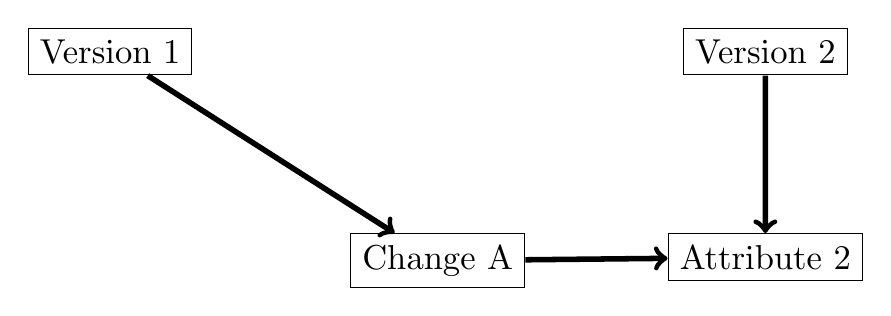
\begin{tikzpicture}[every node/.style={draw, rectangle}]
		\begin{scope}[node distance=20mm and 20mm]
			\node (c) [scale=1.25] at (1,0) {Change A};
			\node (1) [above left=of c, scale=1.25] {Version 1};
			\node (2) [above right=of c, scale=1.25] {Version 2};
			\node (a) [below =of 2, scale=1.25] {Attribute 2};
			
			\draw [line width=2pt,->] (1) -- (c);
			\draw [line width=2pt,->] (c) -- (a);
			\draw [line width=2pt, ->] (2) -- (a);
		\end{scope}
	\end{tikzpicture}
	\caption{Model of the relationships between Versions 1 and 2 when adding an Attribute 2 to Version 2 as a result of Change A}
	\label{AdditionFig}  % the \label command comes AFTER the caption
\end{figure}



\section{INVALIDATION}

The Invalidation operation corresponds to the delete concept found in other applications.  The choice of invalidation over delete results from the policy that, in versioning, data should never be deleted.  In practicality, this may not be particularly feasible due to space limitations and relative validity.  In either case, the change invalidates an attribute in version one, resulting in version two.  Unlike the Addition operation, Invalidation forms a clear relationship between both versions, which can be seen in Figure \ref{InvalidationFig}.  Notice again that since Attribute 1 no longer exists in Version 2, there is no corresponding Attribute 2 to refer to.

From Figure \ref{AdditionFig}, we can see the confusion that could result from requiring explicit relationships between versions and changes in both the Addition and Invalidation operations.  Linking Change A to Version 2 would create a duplicate connection and provides a mechanism to identify when items specifically enter or leave a version.

\begin{figure}[t]
	\centering
	\vspace{0.0in} % normally the command here would be \includegraphics
	%	\includegraphics{figures/Addition.png}
	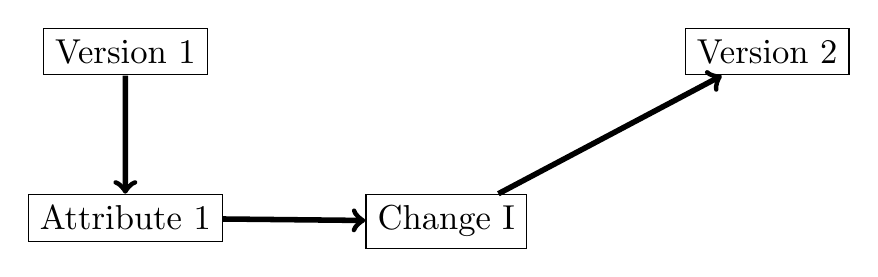
\begin{tikzpicture}[every node/.style={draw, rectangle}]
	\begin{scope}[node distance=15mm and 20mm]
	\node (c) [scale=1.25] at (1,0) {Change I};
	\node (1) [above left=of c, scale=1.25] {Version 1};
	\node (2) [above right=of c, scale=1.25] {Version 2};
	\node (a) [below =of 1, scale=1.25] {Attribute 1};
	
	\draw [line width=2pt,->] (a) -- (c);
	\draw [line width=2pt,->] (c) -- (2);
	\draw [line width=2pt, ->] (1) -- (a);
	\end{scope}
	\end{tikzpicture}
	\caption{Model of the relationships between Versions 1 and 2 when invalidating Attribute 1 from Version 1 as a result of Change I}
	\label{InvalidationFig}  % the \label command comes AFTER the caption
\end{figure}


\section{MODIFICATION}

The final operation is Modification, and it maps a change from one attribute from version one to its corresponding attribute in version two.  The particular type of change in this case is purposely left out in order to allow data producers to subclass and customize the resulting graph to properly reflect the versioning that they desire.

\begin{figure}[b]
	\centering
	\vspace{0.0in} % normally the command here would be \includegraphics
	%	\includegraphics{figures/Addition.png}
	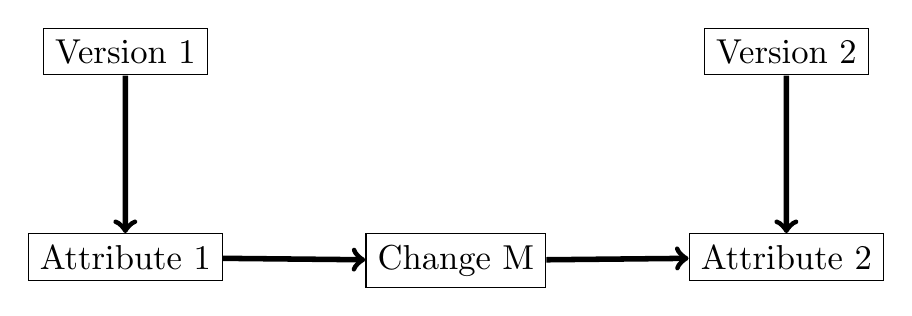
\begin{tikzpicture}[every node/.style={draw, rectangle}]
		\begin{scope}[node distance=20mm and 20mm]
			\node (c) [scale=1.25] at (1,0) {Change M};
			\node (1) [above left=of c, scale=1.25] {Version 1};
			\node (2) [above right=of c, scale=1.25] {Version 2};
			\node (a1) [below =of 1, scale=1.25] {Attribute 1};
			\node (a2) [below =of 2, scale=1.25] {Attribute 2};

			\draw [line width=2pt,->] (a1) -- (c);
			\draw [line width=2pt,->] (c) -- (a2);
			\draw [line width=2pt, ->] (1) -- (a1);
			\draw [line width=2pt, ->] (2) -- (a2);
		\end{scope}
	\end{tikzpicture}
	\caption{Model of the relationships between Versions 1 and 2 when modifying Attribute 1 from Version 1 as a result of Change M, resulting in Attribute 2 from Version 2}
	\label{ModificationFig}  % the \label command comes AFTER the caption
\end{figure}

\section{MULTIPLE LINKED VERSIONS}

Using the construction outlined in the previous three sections, many changes can be compiled together into a graph in a changelog.  After all additions, invalidations, and modifications have been compiled into a single graph, a complete mapping from version one to version two may be developed.  The orientation of the relationships in the graph allows a flow to be created from attributes in version one to corresponding attributes in version two.  Taking version two and performing the same graph construction to a version three results in not only a flow from version two to version three, but also from version one to version three.  As a result, the flow can be used to construct a mapping from version one to version three or any future version.
 % Model Specification
%%%%%%%%%%%%%%%%%%%%%%%%%%%%%%%%%%%%%%%%%%%%%%%%%%%%%%%%%%%%%%%%%%%
%                                                                 %
%                            CHAPTER FOUR                         %
%                                                                 %
%%%%%%%%%%%%%%%%%%%%%%%%%%%%%%%%%%%%%%%%%%%%%%%%%%%%%%%%%%%%%%%%%%%

\chapter{CHANGE METRICS}\label{ch:graph}

\section{Introduction}

Machine computable change logs provides a very powerful means to begin answering basic versioning questions in a formal and systematic manner.
From the change log, a linked data versioning graph can be extracted and the changes counted to communicate how different are two versions.
The data model was constructed to allow a wide variety of ways to connect together versions such that more complex analytics could be performed using the versioning graphs.
The analytics show that producers must be very transparent when communicating the methods data producers use to assess change impacts as shown in Section \ref{gcmd_85}.

When versioning a data set, researchers very rarely ask whether two objects can be compared.
The data producer often establishes the context in which data objects are sufficiently similar---to use terms from FRBR---\textbf{expressions} of the same \textbf{work}.
Confirming the context prior to making version comparisons is fundamental to ensuring that the resulting versioning graph contains meaningful results.
The data sets described in the following section have sufficient context as established by their producers.
Using the data in these data sets, the model from Chapter \ref{ch:model} is instantiated into versioning graphs.
The graphs are encoded into HTML change logs using RDFa and JSON-LD.
These graphs allow for an analysis of the change between versions, which gives insight into the version identifier.
Finally, a version graph is used to classify the kinds of change separating versions of a data set to determine the utility.

\section{Implementing the Versioning Model}

The following subsections detail the steps used to implement a versioning graph using the model defined in Chapter \ref{ch:model} and the challenges encountered.
Section \ref{mapping} goes through the decisions made to align the attributes within the Noble Gas dataset and within the Copper data set.
The alignments create a formula to detect changes and assign them to either an \textbf{add}, \textbf{invalidate}, or \textbf{modify} change.
A change log can then use the assignments to organize a presentation of the change data.
The underlying versioning graph exists as linked data encoded within the change log, but can also appear as explicit linked data statements.
The linked data uses a custom-made versioning ontology (VersOn) to express the data model using the \textit{vo:} namespace.
The procedure within this section defines the process used to create versioning graphs found in all the following sections of this Chapter.

\subsection{Form a Mapping} \label{mapping}

A mapping specifies the method to determine the \textbf{attributes} of a versioning graph and how to compare them.
For spreadsheets and table-based data, row and column indexes initially seem an ideal attribute, but edits often show the contrary.
The Noble Gas data set needed a mapping to align the spreadsheet's columns since 140 columns were removed from the first version.
The remaining columns in the second version no longer had the same column indexes that they did in version 1 so the column headers were used instead.
The Copper data set retains many of the original columns, but their ordering has changed between versions.
In addition, rows must be aligned since both a row and column attribute are necessary to uniquely identify a cell.
The Noble Gas data set split up its rows across eight files, each file representing a separate region of the Earth.
Instead of forming eight versioning graphs or having eight left-hand versions, the files were collected together into a single abstract collection which is then mapped to the right-hand version.
Creating eight versioning graphs would also form eight separate change logs which doesn't make sense since each file forms only a part of the entire work and the second version collects all entries into a single file.
Multiple left-hand versions also doesn't make sense since this creates one change log and graph, but the files are no longer associated with each other.
Cells need to be uniquely identified since this is where a comparison will be made to determine whether a \textbf{modify} change has occurred in a spreadsheet.

Once aligned, determining which attributes have been added, invalidated, or modified is straight-forward.
Attributes which only exist in the original or left-hand version have been invalidated.
More specifically, a set of attributes \(\mathcal{I} = \mathcal{R}_{l} - \mathcal{R}_{r}\) where \(\mathcal{R}_{l}\) and \(\mathcal{R}_{r}\) correspond to the row identifiers of the left-hand and right-hand versions, respectively.
Likewise, a set of attributes \(\mathcal{A} = \mathcal{R}_{r} - \mathcal{R}_{l}\) contain all the added attributes.
Performing the same operations on the columns result in sets of the added and invalidated columns.
A script then iterates over the remaining cells which exist in both versions to determine if they differ, resulting in a \textbf{modify} change.
The unchanged cells form a set of entries which do not appear in a change log or the versioning graph.
The attributes in these sets are then minted into URIs and linked together into the versioning graph, or they can be used to publish a change log.

\subsection{Generate Versioning Graph}

\begin{figure}
	\centering
	\begin{adjustbox}{
			addcode=
				{\begin{minipage}{\width}}
				{
					\caption{Some initial entries from versions 1 and 2 of the Noble Gas data set}
					\label{NobleGraph1}
					\end{minipage}
				},
				rotate=90,
				center}
			\includegraphics[scale=0.39]{figures/NobleVersion.png}
	\end{adjustbox}
\end{figure}
The versioning graphs presented in this section were created by extracting triples from the associated change log which will be covered in Chapter \ref{ch:changelog}.
The statements making up the graph could have alternately been published by writing out the triples directly instead of encoding them into a change log.
Figure \ref{NobleGraph1} displays a subgraph of the Noble Gas data set's versioning graph between versions 1 and 2, highlighting each of the three change operations.
Notice how the versioning graph differs from the provenance graph in Figure \ref{CAM001ProvGraph}.
The versioning graph unpacks the \textit{prov:wasRevisionOf} relationship into explicit components.
These components reveal more detailed differences between version 1 and 2 of CAM001 in the provenance graph which are the differing compilation activities.
\begin{figure}
	\centering
	\begin{adjustbox}{
		addcode=
			{\begin{minipage}{\width}}
			{
				\caption{Provenance graph for the CAM001 entry of the Noble Gas Database.  Other than the labels, the structure of each data object is very much the same.}
				\label{CAM001ProvGraph}
				\end{minipage}
			},
			rotate=90,
			center}
		\includegraphics[scale=0.80]{figures/CAM001v1v2.png}
	\end{adjustbox}
\end{figure}
The change log encoded the triples in RDFa, resulting in the attribute ``AttributeCAM00111v2" to the right of the \textbf{modify} change.
Because RDFa does not naturally support multiple predicates while also conforming to the content structure of the change log, an attribute was created to combine both the row and column identifier for the changing cell.
Separating the attributes would require multiple dedicated HTML tags which don't appear along with content.
Including these tags would diverge from benefits of encoding triples as attributes.
Figure \ref{NobleGraph1} also shows that even though many columns are added when a new row is added, the row identifier can be used to summarize the columns additions.

Another modification to the implementation differs from the original versioning model.
The \textbf{modify} construction defined in the model only covers the case where a single attribute is sufficient to define a change relation.
The \textbf{modification} captured in spreadsheets describes a cell which requires a row and column identifier to indicate uniquely.
The implementation demonstrates that using multiple attributes is an allowable, sometimes necessary, construction.

Listing \ref{NGA} presents the statements in turtle format necessary to express that the entry EGY001 has been added to the data set from Version 1 to Version 2 as shown along the top of Figure \ref{NobleGraph1}.
The namespace for many of the URIs is \textlangle http://rdfa.info/play/\textrangle.
RDFa allows identifiers to refer to an element on the web page, and the web tool which generated the triples from RDFa, therefore, used its URL as a namespace to produce a valid URI.


\begin{listing}
	\begin{minted}[linenos, frame=lines, breaklines]{SPARQL}
<http://rdfa.info/play/Version1> a vo:Version ;
vo:absentFrom <http://rdfa.info/play/AddChange21> .
<http://rdfa.info/play/AddChange21> a <https://orion.tw.rpi.edu/~blee/VersionOntology.owl#AddChange> ;
vo:resultsIn <http://rdfa.info/play/Attribute21> .
<http://rdfa.info/play/Attribute21> a <https://orion.tw.rpi.edu/~blee/VersionOntology.owl#Attribute> ;
rdfs:label "EGY001"
<http://rdfa.info/play/Version2> a vo:Version ;
vo:hasAttribute <http://rdfa.info/play/Attribute21>
	\end{minted}
	\caption{Noble Gas Add in Turtle}
	\label{NGA}
\end{listing}

Figure \ref{CopperGraphVerGraph} shows a similar subgraph from the Copper data set versioning graph.
The graph was assembled using an RDFa change log and also displays a merged attribute on the right side of the \textbf{modify} change.
In the full versioning graph, multiple of each change is present, forming a zipper or ladder-like structure.
As a result, each \textbf{add}, \textbf{invalidate}, or \textbf{modify} change is given separate names for each instantiation.

\begin{figure}
	\centering
	\begin{adjustbox}{addcode={\begin{minipage}{\width}}{
					\caption{Versioning Graph representing the linked data graph with selected entries of additions, invalidations, and modifications.}
					\label{CopperGraphVerGraph}					
					\end{minipage}},rotate=90,center}
		\includegraphics[scale=0.5]{figures/VersioningGraph2.png}%
	\end{adjustbox}
\end{figure}

\subsection{Graphs with Multiple Versions}\label{sec:multiver}

Figures \ref{NobleGraph1} and \ref{CopperGraphVerGraph} depict a comparison between only two versions, but a project can contain more than two objects.
Case in point, a third version of the Noble Gas data set was released on July 11, 2017.
Figure \ref{NobleGraph2} shows a subgraph that contains changes from all three versions of the Noble Gas data set.
\begin{figure}
	\centering
	\begin{adjustbox}{addcode={\begin{minipage}{\width}}{
					\caption{Versioning Graph representing the linked data graph with selected entries of additions, invalidations, and modifications after the publication of the third version.}
					\label{NobleGraph2}					
		\end{minipage}},rotate=90,center}
		\includegraphics[scale=0.48]{figures/NobleVersion2.png}%
	\end{adjustbox}
\end{figure}
From the first to second version of the data, EGY001 becomes introduced as an attribute into the data set.
This entry then undergoes a modification change in columns 29, 31, and 43 when comparing versions two and three.
Entry TUR030 goes through a modification change in column 11 from version one to version two.
The entire row, however, becomes invalidated in version three.


Notice the difference in how Figure \ref{NobleGraph1} and Figure \ref{NobleGraph2} refer to columns.
Figure \ref{NobleGraph1} used linked data extracted from a change log employing RDFa, forcing the row identifier and the column identifier into the same concept.
The way nesting works in RDFa means that ChangeCAM00111 cannot back reference multiple concepts in a single statement, therefore AttributeCAM00111v2 was used to imply CAM001.
Figure \ref{NobleGraph2} used linked data extracted from a JSON-LD encoded change log.
Since the log can use explicit statements, the column identifier refers to the entire column and can be used to identify changes in the same column across multiple rows.

\section{Change Metric} \label{ch:distance}

Use Case 2 addresses the use of versions to communicate how different two objects are.
Many versioning systems use dot-decimal identifiers to signify whether a change is large, medium, or small.
The exact requirements to determine change size differs widely across different domains and applications.
The versioning graph provides a new, more regular method to quantify change between objects using versioning operations.
The work done with GCMD Keywords shows the qualitative relationship between version identifiers and change distance.
Work with the MBVL data set then extends VersOn to give more detailed accounting with the change capture method.

\subsection{Utilized Data Sets}

\subsubsection{Global Change Master Directory Keywords}

The Global Change Master Directory (GCMD) is a metadata repository used by NASA to store records of its available data sets \cite{Miled:2001:GCM:372202.372324}.
They employ a set of keywords to make NASA Earth Science data sets searchable.
These words tag and label datasets into strictly defined categories \cite{GCMDKey}.
GCMD Keywords do not qualify as a standard web ontology since GCMD Keywords do not constitute a class hierarchy.
The management team stored early versions of the keywords in Excel spreadsheets, later using a centralized distribution system, but data is not available prior to June 12, 2012.
The Key Management Service now serves the keywords directly in a variety of formats.
Each version of the keywords, encoded in RDF, was downloaded into separate files.
Only versions from June 12, 2012 and after were available, resulting in 9 version files.
Each keyword corresponds to a unique identifier, and when combined with a web namespace, resolves to a data description of the keyword.
Every identifier can be referred to per version by including the version's number at the web identifier's end, meaning that identifiers are consistent across versions.
The taxonomy uses the concepts \textit{skos:Broader} and \textit{skos:Narrower}, where skos refers to the Simple Knowledge Organization System ontology name space, to form a tree hierarchy \cite{skos}.
The tree's root is the keyword, "Science Keywords."
The data set provides an interesting study case due its long sequence of versions and ready use of linked data technology \cite{Stevens2016}.

\subsubsection{Marine Biodiversity Virtual Laboratory Classifications} \label{sec:MBVL}

The Marine Biodiversity Virtual Laboratory (MBVL), based at Woods Hole Oceanographic Institution, provides data and services for the study of marine biology with an integrative approach \cite{mbvl}.
In the application studied, a choice of algorithm and taxonomy pairings must be tested on a known population in order to estimate their performance with an unknown microbial population.
The original sequences belong only to the species listed in Table \ref{species_table}.
The original population's census is not available to the author, and only the list of species is known, forming the first data set in this section.
These sequences are then grouped and classified by a specific taxonomy and algorithm pairing.
The workflow utilizes two taxonomies, the Ribosomal Database Project (RDP) and the Silva taxonomy.
Using these databases, the SPecies-level IdentificatioN of metaGenOmic amplicons (SPINGO) or the Global Alignment for Sequence Taxonomy (GAST) algorithms assign taxonomic ranks to each sequence.
The process produces four data sets, each using the same grouping identifiers and having the same size in each group.
Since the data sets have the same number of sequences, the primary differences between the data sets are the ranks assigned to each sequence.

\begin{table}
	\caption{List of species in the original population.}
	\label{species_table}
	\centering
	\setlength{\tabcolsep}{2pt}
	\begin{tabular}{|c|c|c|}
		\hline
		Acinetobacter baumannii & Actinomyces odontolyticus & Bacillus cereus \\
		Bacteroides vulgatus & Clostridium beijerinckii & Deinococcus radiodurans \\
		Enterococcus faecalis & Escherichia coli & Helicobacter pylori \\
		Lactobacillus gasseri & Listeria monocytogenes & Neisseria meningitidis\\
		Porphyromonas gingivalis & Propionibacterium acnes & Pseudomonas aeruginosa \\
		Rhodobacter sphaeroides & Staphylococcus aureus & Staphylococcus epidermidis\\
		Streptococcus agalactiae & Streptococcus mutans & Streptococcus pneumoniae \\
		\hline
	\end{tabular}
\end{table}

\section{Global Change Master Directory}

\subsection{Global Change Master Directory Versioning Graph}

The Global Change Master Directory establishes the context that each \textbf{manifestation} of their keyword list is related versions.
Since the unique identifier for each keyword remains the same across versions, the unique keyword identifier can be used to align a mapping across versions.
\textbf{Additions} and \textbf{invalidations} are detected by checking an identifier's presence within both versions.
A \textbf{modification} occurs when a keyword's \textit{skos:Broader} property differs between adjacent versions.
The alignment assumes that there is not reason a keyword's preferred label would change, but still reports a value when it has new entries in the ``notes" property.
A difference indicates that the word has been moved to a different place within the taxonomy since identifiers do not change across versions and a keyword only has one parent concept.
Changes over consecutive versions can be collected into a single graph using the method in Section \ref{sec:multiver} to chain together versioning graphs.
A change log was generated for each pair of consecutive versions in GCMD Keywords and embedded with JSON-LD.
Versioning graphs for each adjacent version was created by extracting JSON-LD from the corresponding change log, and entering the triples into a Fuseki triple store.

\subsection{Connecting Change Counts to Identifiers} \label{gcmd_85}

The \textbf{add}, \textbf{invalidate}, and \textbf{modify} counts for each transition are presented in Figure \ref{GCMDC1}.
The query used to extract the counts is found in Listing \ref{gcmd_list}.
Notice the sharp spike in adds and invalidates when transitioning from version 8.4.1 to 8.5.
The version identifiers indicate that at most a minor or technical change has occurred, but the counts of \textbf{addition} and \textbf{invalidation} changes in this transition is more than triple the counts in either of the previous \textbf{major} transitions.
Not only should a small transition not produce changes of this quantity, but the data set's size is on the order magnitude of the recorded \textbf{invalidates}.
In addition, no \textbf{modifications} are revealed, and even the root node "Science Keywords" has been invalidated.
Further investigation of the root word reveals that the name space for the keywords has changed from HTTP to HTTPS.
To provide context, NASA mandated a transition to secure protocols, and the group changed the name space to ensure the URIs remained resolvable.
Since the identifiers are unique, the new name space means they no longer refer to the same object after the protocol change.
Because the keyword identifiers no longer match, the mapping approach results in the total invalidation of keywords from 8.4.1 and the addition of keywords from 8.5.
The dot decimal identifier for the transition from version 8.4.1 to 8.5 does not match the number of changes in the versioning graph.

\begin{table}
	\caption{Global Change Master Directory Keyword Change Counts}
	\label{table:GCMD_main}
	\centering
	\begin{tabular}{|c|c|c|c|c|}
		\hline
		
		Transition&	Add&	Invalidate&	Modify&	Total\\\hline
		June 12, 2012 to 7.0&	310&	9&	22&	341\\
		7.0 to 8.0&	503&	6&	79&	588\\
		8.0 to 8.1&	277&	28&	22&	327\\
		8.1 to 8.2&	53&	1&	26&	80\\
		8.2 to 8.3&	58&	0&	13&	71\\
		8.3 to 8.4&	53&	0&	1&	54\\
		8.4 to 8.4.1&	86&	13&	8&	107\\
		\hline
	\end{tabular}
\end{table}
\begin{figure}[b]
	\centering
	\includegraphics[scale=0.83]{figures/GCMDChartShort.png}
	\caption[Global Change Master Directory Keywords Change counts up to Version 8.4.1]{Add, Invalidate, and Modify counts from the beginning of the Keyword Management System to Version 8.4.1.}
	\label{GCMDC1}
\end{figure}

%\hfill \break

\begin{listing}
	\begin{minted}[linenos, frame=lines, breaklines]{sparql}
PREFIX vo:<http://orion.tw.rpi.edu/~blee/VersionOntology.owl>
PREFIX rdfs:<http://www.w3.org/2000/01/rdf-schema#>

SELECT ?p (COUNT (DISTINCT ?s) as ?count)
{
?s a ?p .
?p rdfs:subClassOf vo:Change .
} GROUP BY ?p
	\end{minted}
	\caption[Change count query.]{This query compiles the counts for each subclass of Change in a GCMD versioning graph.}
	\label{gcmd_list}
\end{listing}

Changing the mapping method to account for the new namespace provides a pathway to compare the perceived change by the producer as evidenced by the version identifier with the amount of change in the versioning graph.
To do this, the mapping treats identifiers with HTTP and HTTPS the same. 
Differences in change magnitudes become much clearer after controlling for the altered name space in Figure \ref{GCMDC2}.
All revisions are dominated by \textbf{additions}, but major version changes have counts around 300 to 500 while minor revisions are an order of magnitude smaller.
The transition from version 8.4.1 to 8.5 also seems to follow this trend.
The \textbf{additions} in ``8.4 to 8.4.1" in Figure \ref{GCMDC2} numbers almost a hundred, providing evidence that the trend of decreasing order of magnitudes may now continue as the granularity of the version identifier increases.

\begin{table}
	\caption{Difference in Version 8.5 mapping methods}
	\label{table:GCMD_8_5}
	\centering
	\begin{tabular}{|c|c|c|c|c|}
		\hline
		Mapping Method&	Add&	Invalidate&	Move&	Modify\\ \hline
		Standard&	3097&	3031&	0&	0\\
		Silent&	68&	2&	22&	0\\
		Bridged&	68&	2&	22&	3007\\		
		\hline
	\end{tabular}
\end{table}
\begin{figure}%[b]
	\centering
	\includegraphics[scale=.9]{figures/GCMD8_5.png}
	\caption{Add, Invalidate, and Modify counts using different methods of mapping identifiers in Global Change Master Directory Keywords Version 8.4.1 to 8.5.}
	\label{GCMDC2}
\end{figure}


\section{Marine Biodiversity Virtual Laboratory}

\subsection{Variant Versioning Graph}

The experiment conducts activity over two phases in this procedure.
The first phase takes sequences from the original known population and feeds the sequences though a particular algorithm/taxonomy combination to produce a candidate classification.
Since the classifications for the known population sequences are unavailable, there is not sufficient context to perform a valid comparison with the candidate classifications.
The second phase compares the performances of each candidate classification of a algorithm/taxonomy pair.
The use of \textbf{add}, \textbf{invalidate}, and \textbf{modify} varies slightly in this application since all the results use the same sequences.
A versioning graph utilizing just the sequence identifiers would only result in \textbf{modify} changes when taxonomic ranks differ since the sequence identifier exists in both data sets.
The mapping instead uses the sequence identifiers to align comparisons and then the taxonomic rank classification to determine the kind of change.
If the right-hand result specifies more taxonomic ranks, the relationship is an \textbf{addition}.
If the left-hand result is more specific, then the relationship is classified as an \textbf{invalidation}.
If both results have the same precision but the name differs, then the link is a \textbf{modification}.
Otherwise, no change is detected.

Figure \ref{mbvl_chart} shows the changes detected when varying either the taxonomy or the classification algorithm.
\begin{figure}
	\centering
	\includegraphics[scale=0.75]{figures/mbvl_chart.png}
	\caption{Compiled counts of \textbf{adds}, \textbf{invalidates}, and \textbf{modifies} grouped by taxonomic rank across algorithm and taxonomy combinations.}
	\label{mbvl_chart}
\end{figure}
Only the taxonomy or only the classifier differs in each comparison to control for overlapping influences that having both a different taxonomy and classifier may introduce.
Each bar indicates the total number of differences between sequences for a specific kind of change.
The bars are further broken down by the taxonomic rank at which the difference occurred.
For example, in ``Silva vs RDP, Gast", a notable number of classifications differed at the species rank.
The graph also indicates that using the RDP taxonomy often produces more precise classifications since both ``Silva vs RDP, Spingo" and ``Silva vs RDP, Gast" feature a larger number of \textbf{additions} than any other change.
The classifier comparisons feature a high number of \textbf{invalidations}; however, ``RDP, Spingo vs Gast" also displays a higher number of \textbf{modifications} than \textbf{invalidations}.

\section{Version Graph Discussion}

The versioning graph successfully addresses the concerns of Use Case 1 by capturing all the differences within the Noble Gas data set and within the Copper data set into a versioning graph.
Some additional concerns had to be addressed, such as multiple files in a version and dual attribute identification, during the implementation of the versioning model.
The multiple files in the first version of the Noble Gas data set needed to be collected into a single concept in order to preserve the one-to-one relation between versions.
The grouping simplifies the graph structure as well as reduce the complexity of a change log encoding.

In Section \ref{ch:model}, there is only one \textbf{attribute} on each side of the interaction.
Figure \ref{CopperGraphVerGraph}, however, shows two \textbf{attributes} used to characterize the \textit{vo:ModifyChange}.
While the model only shows one \textbf{attribute}, it was found that in some applications, multiple \textbf{attributes} may be necessary to properly model a single change.
The construction does not even need to have the same number \textbf{attributes} on both sides of the \textbf{change}.
The flexibility becomes important when trying to model, for example, a single location entry being split into separate latitude and longitude entries.

The version graph's construction allows multiple versions to be linked together.
The graph provides not only greater continuity than Schema.org's properties, but also greater detail than PROV's versioning properties.
Continuity is important since many versioning linked data alternatives view version change as a single contained \textbf{activity}.
When linking together multiple versions using a versioning graph, the relationship between non-adjacent editions becomes implied in the graph's structure.
The natural pathway between \textbf{attributes} in non-adjacent \textbf{versions} holistically considers the relationships among all \textbf{attributes} along that path.
In comparison, other models only capture activity between the adjacent versions.

The model struggles with discontinuous changes to an \textbf{attribute} across multiple versions.
Since the model does not capture when an \textbf{attribute} doesn't change, it is possible for an \textbf{attribute} in an earlier \textbf{version} to become disconnected from later \textbf{versions} due to inactivity.
For example, in Figure \ref{NobleGraph2}, column 31 of EGY001 becomes modified transitioning into the third version.
If that column underwent no activity in the next transition but changed from version four to five, the connection between all the column 31s would no longer be continuous.
This poses a problem for executing queries in a triple store which rely on graph traversals, but no path exists between disconnected \textbf{attributes}.

\subsection{Version Identification}

The versioning process discovered a discrepancy in the identifier assignment in the GCMD Keywords taxonomy.
The original analysis was intended to determine if dot-decimal identifiers would reflect an order of magnitude division among the change counts of the versioning graph.
According to the \textit{Keyword Governance and Community Guide Document} \cite{gcmd_gov}, ``Full GCMD keywords list releases get a new major version number (e.g., 8.0). Incremental releases for updates to topics, terms, and variables get a new minor version number (e.g., 8.1).”
The change counts for Versions `June 12, 2012' to 8.4.1 demonstrates a threshold of changes necessitating a full keywords list release.
The document does not explain the purpose or distinguishing qualities of versions with a new revision number, 8.4.1.
Version 8.5, however, was named with respect to perceived taxonomy changes and did not consider underlying linked data practice revisions.
The conclusion can be obtained by looking at \ref{GCMDC2} and noticing that the only matching approach without a bar equal to the size of the entire data set is the `Silent' approach.
For a purely URI based comparison in `Standard', Version 8.5 definitely falls under the category of full release since an entirely new list of words is released.
Users using the `Bridged' approach would also see a new full release because all old words have had the URIs edited.
Version name assignment based on producer perception and not allowing users to assess change measures is concerning.
Making sure that data consumers have the ability to assess change in data sets when the requirements for change differs between producer and consumer must be addressed.

The analysis does not to claim that change counts should be the sole mechanism in determining version identifiers.
The counts, however, can provide a more quantitative method to compare version differences.
In Figure \ref{GCMDC1}, the yellow line indicates the total changes made to the data set, performing a similar function as the major/minor/revision version identifier.
Breaking up the changes into types reveals additions dominate manipulations to the data set.
Addition, invalidation, and modification provides deeper insight into how a data set is changing, but some changes can be more impactful than others which this model does not capture.

\subsection{MBVL Analysis}

In Section \ref{ch:distance}, the versioning process was used to compare the performance of different taxonomy and algorithm combinations.
The data set diverges from many of the common understandings of versions since each of the versions are not sequential and are largely independent.
The data set of species names in the initial population would not have produced very meaningful results if applied to the versioning model since it lacked sufficient data to map the other data sets together well.

In Figure \ref{mbvl_chart}, the first set of columns in the Silva taxonomy results are versioned against RDP using the SPINGO algorithm.
The naming reflects the orientation in the versioning graph so Silva forms the left-hand version and RDP would be the right-hand version.
In this comparison, using the RDP taxonomy seems to provide more accurate results, most specifically at the species level.
The taxonomies also disagree fairly often at the species and family ranks.
Switching to the GAST algorithm in the second set of columns, RDP once again demonstrates a noticeably greater accuracy in species classification.
There are also significantly fewer disagreements using the GAST algorithm between the two taxonomies.
Looking at the third set of columns, Silva demonstrates greater accuracy classifications under the SPINGO algorithm than under GAST.
Over four thousand of these entries can be classified to the species level when GAST cannot.
In the fourth set of columns, RDP appears to perform better with SPINGO than GAST.
However, the comparison is dominated by a much larger number of disagreements between almost six thousand entries, primarily at the species rank.
On closer inspection, this disagreement is explained by GAST classifying the species for a number of entries as ``uncultured bacterium".
This analysis presents evidence that using the RDP taxonomy with the SPINGO algorithm will produce the most accurate classification results.

\section{Summary}

The results in this chapter implements the versioning model and demonstrates the process and challenges experienced in this endeavor.
The entries in a data set is separated into groups of \textbf{additions}, \textbf{invalidations}, \textbf{modifications}, and unmodified by their attributes.
The grouping occurs over multiple files in the first version of the Noble Gas data set, and the solution was to collect them into a single unit.
The collection keeps the files as one unit, but does not end up addressing other approaches to multi-part versions.

These operational groups organizes the data into a form to publish into a versioning graph.
The approach used to create the graph involves extracting the linked data from a marked up change log.
The decision resulted in constrained representations of the versioning graph, resulting from demands of the encoding methods.
Graphs created using freer form statements, such as the one in Figure \ref{NobleGraph2}, demonstrate an opportunity enable querying over different dimensions of the data.
Changes for specific columns can be queries as easily as individual rows.

The ability to link changes of multiple versions together results as a side effect of the model construction.
Continuously linked changes opens up avenues of exploration to follow change as it propagates through versions.
While change logs will provide a more focused comparison, a triple store with a multi-version graph would give a view of the work through time.
Considering the Noble Gas data set's versioning graph's size, many versions may be difficult to store with large, volatile data sets.

The MBVL data set demonstrates a case where versioning graphs can be used to compare the performance of different taxonomy/algorithm pairings.
The ability derives from sub-classing each of the add, invalidate, and modify changes to give a better perspective where the pairings differed.
This approach of extending the versioning graph adds domain knowledge to the version comparison and helps contextualize the observed differences.
 % Version Graph
%%%%%%%%%%%%%%%%%%%%%%%%%%%%%%%%%%%%%%%%%%%%%%%%%%%%%%%%%%%%%%%%%%%
%                                                                 %
%                            CHAPTER FIVE                         %
%                                                                 %
%%%%%%%%%%%%%%%%%%%%%%%%%%%%%%%%%%%%%%%%%%%%%%%%%%%%%%%%%%%%%%%%%%%

\chapter{Data Volatility}

\section{Introduction}

Capturing change counts is important but understanding how a data set changes over time is also valuable to users.

Look at Figure \ref{GCMDC1} and notice the different total amounts of change in each version of GCMD Keywords.
The group appears to do significantly less work in updating the data set after Version 8.1, but the appearance only occurs because the versions are disconnected from time.
Once we're able to quantify change, we can begin looking at trends over time.
Data volatility is the likelihood or rate of data change.
Volatility helps explain the 
We want to know if data versions are hiding the actual rate of change

\section{Determining Volatility}

Instead of charting the version changes in evenly wide bars, the versions are spread across time based on the time of publication to the KMS as seen in Figure \ref{GCMDPlot1}.
\begin{figure}%[b]
	\centering
	\includegraphics[scale=0.56]{figures/GCMDPlot1.png}
	\caption[Global Change Master Direcotry counts distributed over time.]{Add counts for all versions of GCMD up to 8.5 evenly distributed over the time of version validity.}
	\label{GCMDPlot1}
\end{figure}
Since each of the versions were dominated by the \textbf{Add} counts, the count is divided by the number of days between the publication of a version on the left side of the line and the release of the replacement version on the right side of the line.
The height of the line on the chart gives the steady rate of change until the release of the new version.
The area underneath the line is the total amount of change the new version introduces.
Since each version packages together all the changes into a single release, the actual change rate is unknown.

Three observable clusters appear in the time aware presentation of the versions, highlighted in Figure \ref{GCMDPlot1Cluster}.
\begin{figure}%[b]
	\centering
	\includegraphics[scale=0.56]{figures/GCMDPlot1_Cluster.png}
	\caption[Global Change Master Directory count distributed over time with clusters marked.]{The change rate of different versions organize into three visible clusters. Cluster 2 denotes a sudden burst of version releases which is notable.}
	\label{GCMDPlot1Cluster}
\end{figure}
According to the Keyword Governance and Community Guide Document \cite{gcmd_gov}, ``Full GCMD keywords list releases get a new major version number (e.g., 8.0). Incremental releases for updates to topics, terms, and variables get a new minor version number (e.g., 8.1).”
The statement explains the activity in Cluster 1 where there are sufficient changes to warrant a full release of the keywords.
Cluster 2 captures the change rate and duration of minor versions, except those from 8.2 to 8.4.1 which are in Cluster 3.
Cluster 3 demonstrates a flurry of activity occurring between June 7, 2016, to August 2, 2016.
Considering the previous pattern of taking at least six months between releases, three minor version releases within as many months is highly unusual.

An immediate concern is that Cluster 3 does not result from a sudden burst of activity, necessitating rapid version replacement.
An inquiry into reasoning behind the successive publication returned a statement that the government customer had requested the action.
Another way to dig into the behavior is to look into the impact assessments accompanying the versions.
Impact assessments prior to Version 8.5 are not publicly available, and only assessments for versions 8.2, 8.3, and 8.4 were received upon request.
Of the 6 requests affecting Earth Science Keywords in 8.2, published June 7, 2016, 4 were made in 2014, and the remaining 2 were made in 2015.
Version 8.3 had 8 entries in its impact assessment with 7 entries originating in 2014, and the remaining entry from 2015.
The 6 entries 8.4’s impact assessment has 5 entries from 2008 and 1 entry from 2015.
The data is collected in Table \ref{table:GCMD_old}.
\begin{table}
	\caption{Global Change Master Directory versions with old start time changes.}
	\label{table:GCMD_old}
	\centering
	\begin{tabular}{|c|c|c|c|c|}
		\hline
		Version Name&	Publish Date&	2008&	2014&	2015\\ \hline
		8.2&	June 7, 2016&	0&	4&	2\\
		8.3&	June 21, 2016&	0&	7&	1\\
		8.4&	July 7, 2016&	5&	0&	1\\
		\hline
	\end{tabular}
\end{table}


\section{Earth Observing Laboratory}

The Earth Observing Laboratory (EOL) of the National Center for Atmospheric Research (NCAR) distributes small data sets, around 10-12 files per data set, regarding lower atmospheric data beginning in 2005 \cite{EOL}.
The EOL data sets are somewhat unique in the data set size means management often does not require automation.
In mid-2014, EOL began assigning versions to stored data sets.
When receiving a new version of a data set from a researcher, the practice is to upload the entire new data set, and replace all old files.

Of the 1335 data sets maintained by EOL with versions, only 180 data sets had more than one version.  
The full distribution of version counts is in Table \ref{table:EOL_Versions}
\begin{table}
	\caption{Version Content of Earth Observing Laboratory Data Sets}
	\label{table:EOL_Versions}
	\centering
	\begin{tabular}{|c|c|}
		\hline
		Number of Versions& Number of Data Sets\\ \hline
		1&	1155\\
		2&	141\\
		3&	26\\
		4&	10\\
		5&	3\\
		Total&	1335\\
		\hline
	\end{tabular}
\end{table}
The 1155 other data sets were filtered out since change counts could not be computed for single-version collections.
Since all the files are replaced on an update and a unique file identifier like a hash sum was unavailable, file matching between versions rely on filenames to perform change mappings.
For all files that matched names across versions, the relation was classified as \textbf{Modify}.  
The approach will over-count the number of modifications, but provides an upper bound on the data set volatility in the repository.  
Each count is then normalized by the number of files in the previous version to standardize comparison between data sets regardless of data set size.  
The average for each data set is taken for each change type.

\section{EOL Versioning Behavior}

Given that EOL replaces the entire old data set when updating, the expected behavior of the transitions would be \textbf{Modifies} concentrating close to 1 and \textbf{Adds} and \textbf{Invalidates} distributed close to 0.
The assumption is that researchers have little reason to change the file naming scheme.
The data surprisingly indicates that data sets in EOL primarily gravitate towards \textbf{Addition} and \textbf{Invalidation} values of 1.
\textbf{Modify} counts score more close to 0 in a complete reversal of expectations.

Figure \ref{EOL_Adds} shows the distribution of \textbf{Add} scores.
\begin{figure}%[b]
	\centering
	\includegraphics[scale=.43]{figures/Eol_Adds.png}
	\caption{Distribution of average normalized Add counts for each data set in Eath Observing Laboratory.}
	\label{EOL_Adds}
\end{figure}
The primary feature of the chart is the bar situated in the `[0.9-1' range, meaning that about 45 data sets add a number of files equal to the original size of the data set.
Secondary features include the bars on the far right and far left of the chart, but the bar on the right side is a collection of outliers.
In the outlier data sets, the size of the data set increased drastically compared to the behavior of other data sets managed by EOL.
Outliers are determined by collecting values above 1.5 times the interquartile range (IQR) showing in Table \ref{table:EOL_Change}.
\begin{table}
	\caption{Normalized Change Statistics}
	\label{table:EOL_Change}
	\centering
	\begin{tabular}{|c|c|c|c|}
		\hline
		Stat&	Add&	Invalidate&	Modify\\ \hline
		Mean&	0.714312707&	0.654819294&	0.345180706\\
		Std. Dev&	0.509878564&	0.420093557&	0.420093557\\
		Min&	0&	0&	0\\
		Q1&	0.28635075&	0.142857&	0\\
		Med&	0.9146635&	0.9642855&	0.0357145\\
		Q3&	1.00358625&	1&	0.857143\\
		Max&	54.25&	1&	1\\
		IQR&	0.7172355&	0.857143&	0.857143\\
		\hline
	\end{tabular}
\end{table}
A more muted distribution appears around the 0.5 mark where data sets grow more gradually.

The normalized \textbf{Invalidation} score in Figure \ref{EOL_Invs} shows a majority of data sets removing all or almost all files in the data set.
\begin{figure}%[b]
	\centering
	\includegraphics[scale=.6]{figures/Eol_Inv.png}
	\caption{Distribution of average normalized Invalidate counts for each data set in Eath Observing Laboratory.}
	\label{EOL_Invs}
\end{figure}
Coupled with the information that a quarter of the data sets added close to the original data sets' size of files suggests that the entire data set is being replaced.
\textbf{Invalidations} do not have outliers since only files within the data set can be removed.
The data is extremely biased with only 0.04 separating the median and maximum value.
From Table \ref{table:EOL_Change}, at least a quarter of values are 1.
Figure \ref{EOL_Invs} also shows a muted distrubtion around 0.5.

Figure \ref{EOL_Mods}, representing the normalized \textbf{Modify} distribution, is almost a mirror of the \textbf{Invalidation} chart.
\begin{figure}%[b]
	\centering
	\includegraphics[scale=.6]{figures/Eol_Mod.png}
	\caption{Distribution of average normalized Modify counts of each data set in Eath Observing Laboratory.}
	\label{EOL_Mods}
\end{figure}
The right bar is specifically cut off to capture only 0s, showing that almost a majority of data sets modify 0 files, having 0 files that share names between versions.
The distribution is consistent with a practice of removing all the files in a data set and replacing the files with a new data set using different filenames.
The second feature of this graph shows around 40 data sets in which all or almost all files match across versions.
A small spike of data sets are centralized around 0.5, very much like the other normalized change graphs.

The high concentration of data sets towards 1 in \textbf{additions} and \textbf{invalidations} suggests a more complicated interaction within the data sets.
Individually, the normalized distributions do not show the connection between all three changes since the changes share a common feature, the version transition the changes describe.
Together, the AIM changes create a coordinate in three dimensional space, showing the inter-relation of the changes. 
Figure \ref{EOL_AIM} shows a scatter plot grouping unnormalized change counts for each version.
\begin{figure}%[b]
	\centering
	\includegraphics[scale=.6]{figures/Eol_Versions_3d.png}
	\caption{Distribution of average normalized Modify counts of each data set in Eath Observing Laboratory.}
	\label{EOL_AIM}
\end{figure}
Unlike the other charts, the size of the changes are not normalized by data set size, but the values have the log1p function applied to account for a heavy bias towards 12 and 13.
Notice the one-to-one trend between \textbf{Adds} and \textbf{Invalidates} which shows the tendency of data sets to replace every file and assign a new filename.
If the two changes did not co-occur, a normalized \textbf{Add} score of 1 would indicate that data sets tend to double in size instead.
The files are more likely to retain filenames when only a few files in a data set are being modified.

\section{Analysis}

\subsection{Impact Assessment Change Counts}
\begin{table}
	\caption{Differences in VersOn and Impact Assessment metrics}
	\label{table:GCMD_metric}
	\centering
	\begin{tabular}{|r|r|r|r|}
		\hline
		Version & Add & Invalidate & Modify\\ \hline
		8.2(VO)&	53&	1&	26\\
		-8.2(IA)&	48&	0&	4\\
		\hline
		&	\textbf{5}&	\textbf{1}&	\textbf{22}\\
		\hline
		8.3(VO)&	58&	0&	13\\
		-8.3(IA)&	58&	0&	10\\
		\hline
		&	\textbf{0}&	\textbf{0}&	\textbf{3}\\
		\hline
		8.4(VO)&	53&	0&	1\\
		-8.4(IA)&	66&	0&	5\\
		\hline
		&	\textbf{-13}&	\textbf{0}&	\textbf{-4}\\
		\hline
		8.5(VO)&	68&	2&	22\\
		-8.5(IA)&	55&	0&	30\\
		\hline
		&	\textbf{13}&	\textbf{2}&	\textbf{-8}\\						
		\hline
	\end{tabular}
\end{table}

\subsection{Hidden Volatility}

Each version of a data set stored in EOL is assigned three different times, “version publish time,” “version creation time,” and “version modification time.”  
Version publish time indicates the time the version was made available to the public, usually the data set was added to the database.  
Version creation time denotes the moment at which a version designation was given to the collection of files, beginning in mid-2014 when the versioning system was implemented.  
Version modification time indicates the time at which the version metadata was changed.  
Using version publish time most closely resembles the duration of version validity, and the following computations use version publish time.

Some of the data needed to be filtered out to provide valid results.  
Due to a few coding errors in time assignments, 7 versions had to be removed because the durations were negative.  
Duration is measured in days, and the rate of version publication is determined by taking the inverse of the duration.  
To acquire the AIM change rates, the changes are divided by the associated duration for each version.  
Since the rates are closely concentrated at 0, the log of the rates are taken to give the values a more log-normal distribution.  
Values where an AIM change is 0 had to be removed in order to properly apply the log function.  
The remaining number of entries can be found in Table XX.

Since the durations are not normally distributed, but concentrated close to 0, the log of the durations are taken to normalize the data.  
The log function is also applied to the AIM changes to normalize the data.  
The inverse of the log of the duration is taken to acquire the rate of version release.

The Kolomogorov-Smirnov Test was used to determine if the Adds, Invalidates, or Modifies follow a distribution separate from the version publication distribution.  
A difference indicates that the AIM changes exhibit a behavior apart from the version releases.  
As seen in Figures XX, XX, and XX, the distributions of AIM changes over duration are offset due to a larger magnitude of values per version.  
The change rates were translated by the difference in means between the version mean and the associated change mean after log normalization to make the values valid for comparison by the Kolomogorov-Smirnov test.

\begin{figure}%[b]
	\centering
	\includegraphics[scale=.6]{figures/Eol_Add_Ver_Rate.png}
	\caption{Distribution of average normalized Modify counts of each data set in Eath Observing Laboratory.}
	\label{EOL_Add_Ver}
\end{figure}

\begin{figure}%[b]
	\centering
	\includegraphics[scale=.6]{figures/Eol_Inv_Ver_Rate.png}
	\caption{Distribution of average normalized Modify counts of each data set in Eath Observing Laboratory.}
	\label{EOL_Inv_Ver}
\end{figure}

\begin{figure}%[b]
	\centering
	\includegraphics[scale=.6]{figures/Eol_Mod_Ver_Rate.png}
	\caption{Distribution of average normalized Modify counts of each data set in Eath Observing Laboratory.}
	\label{EOL_Mod_Ver}
\end{figure}

\begin{table}
	\caption{Summary of Kolmogorov-Smirnov Test results for Earth Observing Laboratory.}
	\label{table:Eol_KS}
	\centering
	\begin{tabular}{|c|c|c|c|c|}
		\hline
		&	Add&	Invalidate&	Modify&	Versions\\ \hline
		Length&	205&	192&	114&	227\\
		D-Value&	0.12919&	0.14464&	0.19727&	NA\\
		p-Value&	0.05487&	0.02575&	0.005443&	NA\\
		\hline
	\end{tabular}
\end{table}

 % Change Log
%%%%%%%%%%%%%%%%%%%%%%%%%%%%%%%%%%%%%%%%%%%%%%%%%%%%%%%%%%%%%%%%%%%
%                                                                 %
%                            CHAPTER FIVE                         %
%                                                                 %
%%%%%%%%%%%%%%%%%%%%%%%%%%%%%%%%%%%%%%%%%%%%%%%%%%%%%%%%%%%%%%%%%%%

\chapter{DATABASE VERSIONING}

Databases already maintain a part of versioning history with a transactional log.
However, they pose an interesting change in context compared to spreadsheets.
Often version comparisons occur between instances of spreadsheet files, but with databases, modifying transactions do not generate a new instance of the database.
Identifying a version would then need to adapt and link transactions to versions.
This can be done through query based citations as described by Proll and Rauber \cite{Proell2013}.
The transaction log also more specifically states the attribute involved, making detection of new attributes into the database more straightforward.
This addresses a particular concern in spreadsheet rows since their attributes have a tendency to be less consistent.
Since RRUFF already possesses an automatically, web accessible change log, the work in this area focuses primarily on deconstructing their code to hook in the concept model with RDFa. % Analysis
\chapter{DISCUSSION \& CONCLUSION}

\section{Hidden Versioning Cost}

The evidence that generation costs hamstring the availability of change logs with data sets by default grows with the findings in Section \ref{sec:CLA}.
In Table \ref{table:Ng_changelog_table1}, even the plain text change log is twice the size of the data sets the document describes.
The trade-off of sufficient documentation versus available resources comes into play.
In the end, work to bridge versions with the Noble Gas data set is offloaded onto the data consumer when transitioning between versions.
Mitigating the storage and consumption costs becomes the highest priority in getting widespread change log adoption.

The tradeoff becomes especially important because change documentation often does not have immediate value.
Until consumers have a need to refer back to historical data, the documentation goes unused.
The availability of the information allows consumers to trace changes at crucial times, becoming indispensable in the future.
Automated change log production also produces more complete documentation that may not be fully captured by human error.
The ability to address and predict the costs of implementing a versioning system requires a significantly better understanding of data set version behavior and fundamentals. 

\section{Producer/Consumer Versioning Dynamic}

The investigation into GCMD Keywords has demonstrated the importance of investigating beyond sequential version releases.  
The initial hypothesis was that the dominant change count could provide a reliable indicator to differentiate major and minor versions.  
The resulting numbers shows some reflection of the version name in the change counts.  
A more important finding shows that different approaches can be used to evaluate the number of changes in the Version 8.4 to 8.5 transition.  
The difference highlights a barrier between expertise of data producers and consumers within a system.  
Without prior knowledge of the namespace change, the version indicator violates the GCMD Keyword data policy.  
The ability for a consumer to determine the amount of change within a system becomes incredibly important as the associated change document dictates to the data consumer how the producer thinks users should interact with the data.

The GCMD Keyword data set also demonstrates a transparency issue when utilizing a sequential versioning scheme since versions are not bound to a temporal or change count schedule.  
In Figure \ref{GCMDC1}, we can see that there is a sharp drop off in change counts once entering variants of the 8th major release.  
The finding that the change counts do not consistently relate with version identifiers has already been discussed, but the chart is misleading in showing each version equally spaced from the others.  
Temporally, the versions are separated by a variety of durations.  As mentioned in Section \ref{sec:identifier}, the release rate of versions can be artificially controlled, disconnecting the rate of change from time.  
When refactoring time back into the change measurement, we can see very distinct separation in the change rate as well as their conformance with the version identifiers assigned at the end of the change period.  
In particular, we can see in Cluster 2 of Figure \ref{GCMDPlot1Cluster} that versions can be arbitrarily released in quick succession even though work on the changes inside the version began in 2008, 2014, or 2015.  
This finding indicates that version releases cannot be universally trusted to provide a complete picture of the change within a system by itself.

While investigating inconsistencies between change counts found by the change log and those reported by the impact assessment, differences between the metrics became apparent.  
The lack of alignment arose from a difference between the way the community sees and proposes the keywords and the way the keywords are digitally encapsulated and stored in the KMS.  
As a result, the impact assessments do not capture the structural changes that result from additions to the taxonomy.

\section{Hiddent Data Volatility}

The EOL’s small data set size allows it to adopt a comprehensive replacement method.  
The versioning model identified the need for unique file identifiers to determine when files are specifically changed which were not part of the original versioning metadata starting in 2014.  
The process of capturing change within the system using the model naturally led to a set of basic requirements necessary to implement a versioning system.

The 3 dimensional scatter plot in Figure \ref{EOL_AIM} shows a very surprising tendency in EOL data sets.  
While the description of update methods suggests data sets should be modify dominant, many of the versions replace and rename all the files in a version.  
The volatility analysis for these versions show that when a version is made it will likely entirely replace the previous version.  
The trend also suggests a concerning behavior of contributing scientists to transition away from a previously established file naming scheme.

The problem with change hiding is that version releases mask a data set’s true volatility.  
From the Kolomogorov-Smirnov test results, each of the change types demonstrated a different distribution from the visible version release rate.


\section{New Versioning Nomenclature}
Analysis of versioned data sets has revealed three types of data, dependent on the way in which versions are released: single, periodic, and intermittent.
Single version data sets contain data which cannot be replicated or in which modification would entirely invalidate the data.
High energy physics, previously mentioned, and surveillance data fit within this category.
The data sets in this category will usually only experience additions and invalidations since scientists cannot change the data.

Periodic data sets exhibit version releases at regular intervals in time.  Large data collections usually exhibit a regular behavior when they follow a periodic data collection scheme.
The ARM data center releases data at daily intervals, meaning new versions every day.
The reasons that ARM data sets are not overloaded with version numbers is that some operations, in this case new files, are masked to increase the pertinence of each version designation.
The problem that masking additions causes is the actual amount of change within the data set over time also becomes masked.
The data set then appears to be intermittent when it actually undergoes periodic changes.  As seen in GCMD Keywords and EOL, changes are not necessarily evenly distributed among versions.  The changes, as a result, are also not evenly distributed across time.  As mentioned with distributed versioning methods, periodic version releases can be used to control the volatility of a data set by collecting many changes over time before publication.  Periodic data sets expend version identifiers very quickly since they must release a version even if few significant changes have occurred.

The final type of data set follows intermittent versioning which is characterized by releasing versions as appropriate or as necessary.  The data sets are not bound by an established release schedules.  In the intermittent category falls GCMD Keywords, the Copper data set, and the Noble Gas data set.  Irregular version releases allows data managers the freedom to reduce the number of versions necessary to manage the data set.  When data managers wait too long to release a new version, the number of changes in a single transition can overwhelm methods to track modifications to the data as seen in the Noble Gas data set.  Since intermittent versions are not released based on time, it is very important that versions are released based on some other quantitative measure of change.  Failing to do so invites unclear or worse arbitrary distinction between versions.  GCMD Keywords define clear requirements for major and minor version releases, but the governance document does not explain the requirements for sub-minor versions which occasionally appear in the keyword repository.

Each data set type can additionally be sub-divided into two categories based on the observations made with the AIM model: Add dominant and Modify dominant.  In the data sets currently studied, none exhibit behavior suggesting an Invalidate dominant data set.  A data set is either Add or Modify dominant when a majority of versions have a majority of either Adds or Modifies.  Add dominance indicates that the data is primarily growing while Modify dominance shows that a data set’s coverage is primarily stable but occasionally undergoes adjustments.  The GCMD Keywords is an example of an Add dominant data set since all its version transitions are comprised of new concepts.  The Noble Gas data set shows modify dominance.

\section{Conclusion}

Change analysis for data sets need a great amount of work as big data sets become more common.
Terms and practices need to be standardize and formalized which begins with producing discoverable and consumable change documentation.
The procedures explored showed promise using linked data models, but suffered from size bloating necessary to make the documents machine consumable.
Once computable, producers can begin providing better quantitative measure for change in data, but analysis has shown that the perceived change may differ depending on the consumer of the data set.
The experience highlights an obscured dynamic in change information between data producers and data consumer in which producers often dictate the means of evaluating version change.
Diverging from version-primary practices and including more detailed change accounting becomes a priority after discovering that versions can hide trends in the actual change rate.
The difference between data set change rate and behavior suggests that future research is necessary to determine if the differences indicate versioning practices also need to be different. % Discussion & Conclusion
%%%%%%%%%%%%%%%%%%%%%%%%%%%%%%%%%%%%%%%%%%%%%%%%%%%%%%%%%%%%%%%%%%%
%                                                                 %
%                            CHAPTER SIX                          %
%                                                                 %
%%%%%%%%%%%%%%%%%%%%%%%%%%%%%%%%%%%%%%%%%%%%%%%%%%%%%%%%%%%%%%%%%%%

\chapter{MBVL CLASSIFICATION}

\section{Versioning Graph}

The experiment undergoes two phases of comparison in this procedure.
The first phase compares the initial species content with the classifications by a particular algorithm/taxonomy combination.
Since the classification results from a population selected according to the initial species list, these two datasets share a common provenance.
However, the list cannot be used in place of the classifier results because not only does it have only 21 entries, but also it does not have a clear correspondence with the DNA chains sent to the classifier.
As a result, these two sets are no versions of each other, and versioning results will have weak implications.
A labeling of the initial input data, alternatively would be considered a version of the results, but that data product is not available.

Each taxonomy and classifier combination outputs a taxonomic classification for each entry from the same source.
Shared input data indicates the results share common provenance.
The classifications also share the same workflow step because their results have similar formats, reporting a specific taxonomic name for each entry.
Since classifications occur over the same set of entries, their identifiers can be used to match outputs together for comparison.
However, the classifiers do not identify entries to the same specificity.
If it determines that the confidence at a particular rank is too low, it marks that level as ambiguous and computes no further ranks.
As a result, versioning can determine additions and invalidations based on whether a classifier can ascertain more or less of an entry's taxonomic name.
This method of mapping the versions together allows the results to give insight into the accuracy of different algorithm and taxonomy combinations.

\begin{figure}
	\centering
	\includegraphics[scale=0.80]{figures/mbvl_chart.png}
	\caption{Compiled counts of adds, invalidates, and modifies grouped by taxonomic rank across algorithm and taxonomy combinations.}
	\label{mbvl_chart}
\end{figure} % Future Work
%%%%%%%%%%%%%%%%%%%%%%%%%%%%%%%%%%%%%%%%%%%%%%%%%%%%%%%%%%%%%%%%%%%
%                                                                 %
%                           BIBLIOGRAPHY                          %
%                                                                 %
%%%%%%%%%%%%%%%%%%%%%%%%%%%%%%%%%%%%%%%%%%%%%%%%%%%%%%%%%%%%%%%%%%%

%This method produces a numbered bibliography where the numbers
%correspond to the \cite commands in the text. See the LaTeX manual.
%
\specialhead{REFERENCES}
\begin{singlespace}
\bibliographystyle{References/IEEEtran}
\bibliography{References/References}
\end{singlespace}

% Note that, if you wish, you can use BibTeX to create your bibliography
% from a database. See section 5.6.2 of Memo RPI.110 for information.
%%% Local Variables:
%%% mode: latex
%%% TeX-master: t
%%% End:
 % bibliography
%%%%%%%%%%%%%%%%%%%%%%%%%%%%%%%%%%%%%%%%%%%%%%%%%%%%%%%%%%%%%%%%%%%
%                                                                 %
%                            APPENDICES                           %
%                                                                 %
%%%%%%%%%%%%%%%%%%%%%%%%%%%%%%%%%%%%%%%%%%%%%%%%%%%%%%%%%%%%%%%%%%%

\appendix    % This command is used only once!
%\addcontentsline{toc}{chapter}{APPENDICES}             %toc entry  or:
\addtocontents{toc}{\parindent0pt\vskip12pt APPENDICES} %toc entry, no page #

\chapter{NOBLE GAS CHANGE LOG GENERATOR VERSION 1 TO 2} \label{app:noble12}
\begin{minted}[linenos, frame=lines, baselinestretch=1.2, breaklines]{python}
from os.path import join, dirname, abspath, isfile
from os import sep as separator
import xlrd, sys, json
import glob
import re


def index_convert(index1):
	if index1 < 17:
		return index1
	elif index1 < 24:
		return index1+1
	elif index1 < 26:
		return 26+(3*(index1-24))
	elif index1 < 28:
		return 44+(3*(index1-26))
	elif index1 < 32:
		return 53+(9*(index1-28))
	elif index1 < 36:
		return 88+(2*(index1-32))
	elif index1 < 38:
		return 95+(4*(index1-36))
	elif index1 < 41:
		return 102+(2*(index1-38))
	elif index1 < 43:
		return 112+(2*(index1-41))
	elif index1 == 43:
		return 172
	elif index1 < 50:
		return 174+(3*(index1-44))
	elif index1 < 54:
		return 191+(index1-50)
	else:
		print 'Error: Out of bounds'
		return -1

def test_alignment():
	for i in range(0, 54):
		print 'version2: {:5} version1: {:5}'.format(i, index_convert(i))

def compare_print(mode, key, val1, val2, v1_file, v1_index = 0, v2_index = 0, changelog = None):
	if changelog:
		if mode == 'r':
			out = u'''        <tr  about="Change{}{}" typeof="vo:ModifyChange">
          <td align="right" rev="vo:Undergoes" resource="v1:Attribute{}{}v1" typeof="vo:Attribute">{:2}({})</td>
          <td property="vo:resultsIn" resource="v2:Attribute{}{}v2" typeof="vo:Attribute">{:2}</td>
          <td>{:>10}</td>
          <td>{:>10}</td>
          <span about="Version1" property="vo:hasAttribute" resource="v1:Attribute{}{}v1"></span>
          <span about="Version2" property="vo:hasAttribute" resource="v2:Attribute{}{}v2"></span>
        </tr>\n'''.format(key, v2_index, key, v1_index, v1_index, v1_file, key, v2_index, v2_index, val1, val2, key, v1_index, key, v2_index)
		elif mode == 'j':
			out = u'''        <tr  id="ModifyChange{}{}">
          <td align="right">{:2}({})</td>
          <td>{:2}</td>
          <td>{:>10}</td>
          <td>{:>10}</td>
          <script type="application/ld+json">\n'''.format(key, v2_index, v1_index, v1_file, v2_index, val1, val2)
		elif mode == 't':
			out = u"{:2}({})\t{:2}\t{:>10}\t{:>10}\n".format(v1_index, v1_file, v2_index, val1, val2)
		elif mode == 'u':
			out = u"""<http://example.com/NG/Version1> vo:hasAttribute <http://example.com/NG/Version1/%s> ;
        vo:hasAttribute <http://example.com/NG/Version1/Column%i> .
<http://example.com/NG/Version1/%s> a vo:Attribute ;
        vo:undergoes <http://example.com/Changelog#ModifyChange%s%i> .
<http://example.com/NG/Version1/Column%i> a vo:Attribute ;
        vo:undergoes <http://example.com/Changelog#ModifyChange%s%i> .
<http://example.com/Changelog#ModifyChange%s%i> a vo:ModifyChange ;
        vo:resultsIn <http://example.com/NG/Version2/%s> ;
        vo:resultsIn <http://example.com/NG/Version2/Column%i> .
<http://example.com/NG/Version2> vo:hasAttribute <http://example.com/NG/Version2/%s> ;
        vo:hasAttribute <http://example.com/NG/Version2/Column%i> .

"""%(key, v1_index, key, key, v2_index, v1_index, key, v2_index, key, v2_index, key, v2_index, key, v2_index)
		changelog.write(out.encode('utf8'))
		if mode == 'j':
			json1 = {
"@context":context,
"@type":"vo:Attribute" ,
"@id":"".join(["http://ngdb.com/v1/Attribute", key, str(v1_index)]) ,
"label":key ,
"undergoes":"".join([host, "ModifyChange", key, str(v2_index)]) ,
"@reverse" :    { "hasAttribute" : "Version1" }
}
			json2 = {
"@context":context,
"@type":"vo:ModifyChange",
"@id":"".join([host, "ModifyChange", key, str(v2_index)]) ,
"resultsIn":"".join(["http://ngdb.com/v2/Attribute", key, str(v2_index)])
}
			json3 = {
"@context":context,
"@type":"vo:Attribute" ,
"@id":"".join(["http://ngdb.com/v2/Attribute", key, str(v2_index)]) ,
"label":key ,
"@reverse" :    { "hasAttribute" : "Version2" }
}
			json.dump([json1, json2, json3], changelog, indent=4, sort_keys=True)
			changelog.write('''
          </script>
        </tr>
''')
	else:
		print '{:5}  version1: {:10} version2: {:10}'.format(key, val1, val2)

labels = {17:"SAMPLING - DEPTH - >,<",
		  25:"[He] - ppm - >,<", 27:"[He] - ppm - err", 28:"[He] - mkcc/ - >,<", 30:"[He] - mkcc/ - err", 31:"[He] - mol/ - >,<", 32:"[He] - mol/ - L H2O", 33:"[He] - mol/ - err",
		  34:"[He+Ne] - ppm - >,<", 35:"[He+Ne] - ppm", 36:"[He+Ne] - ppm - err", 37:"[He+Ne] - mkcc/ - >,<", 38:"[He+Ne] - mkcc/ - g H2O", 39:"[He+Ne] - mkcc/ - err", 40:"[He+Ne] - mol/ - >,<", 41:"[He+Ne] - mol/ - L H2O", 42:"[He+Ne] - mol/ - err",
		  43:"[Ne] - ppm - >,<", 45:"[Ne] - ppm - err", 46:"[Ne] - mkcc/ - >,<", 48:"[Ne] - mkcc/ - err", 49:"[Ne] - mol/ - >,<", 50:"[Ne] - mol/ - L H2O", 51:"[Ne] - mol/ - err",
		  52:"[20Ne] - ppm - >,<", 54:"[20Ne] - ppm - err", 55:"[20Ne] - mkcc/ - >,<", 56:"[20Ne] - mkcc/ - g H2O", 57:"[20Ne] - mkcc/ - err", 58:"[20Ne] - mol/ - >,<", 59:"[20Ne] - mol/ - L H2O", 60:"[20Ne] - mol/ - err",
		  61:"[Ar] - ppm - >,<", 63:"[Ar] - ppm - err", 64:"[Ar] - mkcc/ - >,<", 65:"[Ar] - mkcc/ - g H2O", 66:"[Ar] - mkcc/ - err", 67:"[Ar] - mol/ - >,<", 68:"[Ar] - mol/ - L H2O", 69:"[Ar] - mol/ err",
 		  70:"[Kr] - ppm - >,<", 72:"[Kr] - ppm - err", 73:"[Kr] - mkcc/ - >,<", 74:"[Kr] - mkcc/ - g H2O", 75:"[Kr] - mkcc/ - err", 76:"[Kr] - mol/ - >,<", 77:"[Kr] - mol/ - L H2O", 78:"[Kr] - mol/ err",
		  79:"[Xe] - ppm - >,<", 81:"[Xe] - ppm - err", 82:"[Xe] - mkcc/ - >,<", 83:"[Xe] - mkcc/ - g H2O", 84:"[Xe] - mkcc/ - err", 85:"[Xe] - mol/ - >,<", 86:"[Xe] - mol/ - L H2O", 87:"[Xe] - mol/ err",
		  89:"3He/4He - (R/Ra)me - err", 91:"3He/4He - (R/Ra)corr - err", 93:"3He/4He - Rme - E-8 - err", 96:"3He/4He - Rcorr - E-8 - err", 97:"Rank",
		  98:"He/Ne - >,<", 100:"He/Ne - >,<", 101:"4He/20Ne - >,<", 103:"4He/20Ne - err", 105:"20Ne/22Ne - err", 107:"21Ne/22Ne - (xE-2) - err", 108:"21Ne/20Ne", 109:"21Ne/20Ne - err",
		  110:"22Ne/20Ne", 111:"22Ne/20Ne - err", 113:"38Ar/36Ar - err", 115:"40Ar/36Ar - err", 116:"delta(40Ar)rad", 117:"delta(40Ar)rad - err",
		  118:"He/Ar - He/ - /Ar(air) - >,<", 119:"He/Ar - He/ - /Ar(air)", 120:"He/Ar - He/ - /Ar(air) - err", 121:"He/Ar - 4He/ - /36Ar - >,<", 122:"He/Ar - 4He/ - /36Ar", 123:"He/Ar - 4He/ - /36Ar - err",
		  124:"He/Ar - 4He/ - /40Ar(air) - >,<", 125:"He/Ar - 4He/ - /40Ar(air)", 126:"He/Ar - 4He/ - /40Ar(air) - err",
		  127:"f(He)=(He/Ar)s/(He/Ar)air - >,<", 128:"f(He)=(He/Ar)s/(He/Ar)air", 129:"f(He)=(He/Ar)s/(He/Ar)air - err",
		  130:"Ne/Ar - Ne/ - /Ar(air) - >,<", 131:"Ne/Ar - Ne/ - /Ar(air)", 132:"Ne/Ar - Ne/ - /Ar(air) - err", 133:"Ne/Ar - 20Ne/ - /36Ar - >,<", 134:"Ne/Ar - 20Ne/ - /36Ar", 135:"Ne/Ar - 20Ne/ - /36Ar - err",
		  136:"Ne/Ar - 20Ne/ - /40Ar(air) - >,<", 137:"Ne/Ar - 20Ne/ - /40Ar(air)", 138:"Ne/Ar - 20Ne/ - /40Ar(air) - err", 139:"Ne/Ar - 22Ne/ - /36Ar - >,<", 140:"Ne/Ar - 22Ne/ - /36Ar", 141:"Ne/Ar - 22Ne/ - /36Ar - err",
		  142:"Ne/Ar - 22Ne/ - /40Ar(air) - >,<", 143:"Ne/Ar - 22Ne/ - /40Ar(air)", 144:"Ne/Ar - 22Ne/ - /40Ar(air) - err",
		  145:"f(Ne)=(Ne/Ar)s/(Ne/Ar)air - >,<", 146:"f(Ne)=(Ne/Ar)s/(Ne/Ar)air", 147:"f(Ne)=(Ne/Ar)s/(Ne/Ar)air - err",
		  148:"Kr/Ar - Kr/ - /Ar(air) - >,<", 149:"Kr/Ar - Kr/ - /Ar(air)", 150:"Kr/Ar - Kr/ - /Ar(air) - err", 151:"Kr/Ar - 84Kr/ - /36Ar - >,<", 152:"Kr/Ar - 84Kr/ - /36Ar", 153:"Kr/Ar - 84Kr/ - /36Ar - err",
		  154:"Kr/Ar - 84Kr/ - /40Ar(air) - >,<", 155:"Kr/Ar - 84Kr/ - /40Ar(air)", 156:"Kr/Ar - 84Kr/ - /40Ar(air) - err",
		  157:"f(Kr)=(Kr/Ar)s/(Kr/Ar)air - >,<",158:"f(Kr)=(Kr/Ar)s/(Kr/Ar)air", 159:"f(Kr)=(Kr/Ar)s/(Kr/Ar)air - err",
		  160:"Xe/Ar - Xe/ - /Ar(air) - >,<", 161:"Xe/Ar - Xe/ - /Ar(air)", 162:"Xe/Ar - Xe/ - /Ar(air) - err", 163:"Xe/Ar - 132Xe/ - /36Ar - >,<", 164:"Xe/Ar - 132Xe/ - /36Ar", 165:"Xe/Ar - 132Xe/ - /36Ar - err",
		  166:"Xe/Ar - 132Xe/ - /40Ar(air) - >,<", 167:"Xe/Ar - 132Xe/ - /40Ar(air)", 168:"Xe/Ar - 132Xe/ - /40Ar(air) - err",
		  169:"f(Xe)=(Xe/Ar)s/(Xe/Ar)air - >,<", 170:"f(Xe)=(Xe/Ar)s/(Xe/Ar)air", 171:"f(Xe)=(Xe/Ar)s/(Xe/Ar)air - err",
		  173:"H2 - >,<", 175:"H2 - ppm - err", 176:"O2 - >,<", 178:"O2 - ppm - err", 179:"N2 - >,<", 181:"N2 - ppm - err", 182:"CO2 - >,<", 184:"CO2 - ppm - err", 185:"CH4 - >,<", 187:"CH4 - ppm - err",
		  188:"H2S - >,<", 190:"H2S - ppm - err"}

context = "https://orion.tw.rpi.edu/~blee/provdist/GCMD/VO.jsonld"
host = "http://orion.tw.rpi.edu/~blee/provdist/NobleGas/changelog_json.html#"
#test_alignment()


#print v2_row[0].value
#print indicator_map[v2_row[0].value]

#v1_workbook = xlrd.open_workbook(v1_file)
#v1_sheet = v1_workbook.sheet_by_index(0)
#v1_row = v1_sheet.row(4)

def write_modify(r1, r2, workbook, f_out, mode):
	if mode == 'r':
		out = u'''  <div about="Version1" rel="vo:hasAttribute">
    <div resource="v2:%s" typeof="vo:Attribute">
      <span style="font-weight:bold" property="http://www.w3.org/2000/01/rdf-schema#label">%s</span>
      <table rel="vo:Undergoes">
'''%(r2[0].value, r2[0].value)
	elif mode == 'j':
		out = u'''
    <div about="v2:%s">
      <span style="font-weight:bold" property="http://www.w3.org/2000/01/rdf-schema#label">%s</span>
      <table>
'''%(r2[0].value, r2[0].value)
	elif mode == 't':
		out = u"%s\n"%(r2[0].value)
	elif mode == 'u':
		out = u""

	if mode == 'r' or mode == 'j':
		out = out+'''        <tr>
          <th>Column v1</th>
          <th>Column v2</th>
          <th>Version 1</th>
          <th>Version 2</th>
        </tr>\n'''
	elif mode == 't':
		out = out+"Column v1\tColumn v2\tVersion 1\tVersion 2\n"
	f_out.write(out.encode('utf8'))
		#print '# Searching...'
		#print '# Comparing...'
	for i in range(0,54):
		if r2[i].value != r1[index_convert(i)].value:
			#compare_print(j, v1_row[index_convert(j)].value, v2_row[j].value)
			compare_print(mode, r2[0].value, r1[index_convert(i)].value, r2[i].value, workbook.split('/')[-1], index_convert(i), i, f_out)
	if mode == 'r' or mode == 'j':
		f_out.write('  </table></div><br>\n')
	elif mode == 't' or mode == 'u':
		f_out.write("\n")

def write_removed(v2, col, row, f_out, mode):
	if mode == 'r' or mode == 'j':
		f_out.write('''
      <h3>Columns invalidated by %s</h3>
      <table about="Version2">
'''%(v2.split('/')[-1]))
	elif mode == 't':
		f_out.write("\nColumns invalidated by %s\n"%(v2.split('/')[-1]))

	print "Removed Column"
	for i in col:
        	v1_value = labels.get(i, "")
		if mode == 'r':
			out = u'''        <tr resource="InvlidateChange%i" rev="vo:invalidatedBy" typeof="vo:InvalidateChange">
		<td resource="Attribute%i" rev="vo:Undergoes" typeof="vo:Attribute">%i</td>
          <td about="Attribute%i" property="http://www.w3.org/2000/01/rdf-schema#label">%s</td>
          <span about="Version1" property="vo:hasAttribute" resource="Attribute%i"/>
        </tr>
'''%(i, i, i, i, v1_value, i)
		elif mode == 'j':
			out = u'''        <tr id="InvlidateChange%i" about="InvlidateChange%i">
          <td>%i</td>
          <td>%s</td>
          <script type="application/ld+json">
'''%(i, i, i, v1_value)
		elif mode == 't':
			out = u"%i\t%s\n"%(i, v1_value)
		elif mode == 'u':
			out = u"""<http://example.com/NG/Version1> vo:hasAttribute <http://example.com/NG/Version1/Column%s> .
<http://example.com/NG/Version1/%s> vo:undergoes <http://example.com/Changelog#InvalidateChange%i> .
<http://example.com/Changelog#InvalidateChange%i> a vo:InvalidateChange ;
	vo:invalidatedBy <http://example.com/NG/Version2> .

"""%(i, i, i, i)
		f_out.write(out.encode('utf8'))
		if mode == 'j':
			json1 = {
"@context":context,
"@type":"vo:Attribute" ,
"@id":"".join(["http://ngdb.com/v1/Attribute", str(i)]) ,
"label": v1_value,
"undergoes":"".join([host, "InvalidateChange", str(i)]) ,
"@reverse" :    { "hasAttribute" : "Version1" }
}
			json2 = {
"@context":context,
"@type":"vo:InvalidateChange" ,
"@id": "".join([host, "InvalidateChange", str(i)]) ,
"invalidatedBy"  :   "Version2"
}
			json.dump([json1, json2], f_out, indent=4, sort_keys=True)
			f_out.write('''
          </script>
        </tr>
''')
			

	if mode == 'r' or mode == 'j':
		f_out.write('''      </table>
      <h3>Rows invalidated by %s</h3>
      <table about="Version2">
'''%(v2.split('/')[-1]))
	elif mode == 't':
		f_out.write("\nRows invalidated by %s\n"%(v2.split('/')[-1]))
	elif mode == 'u':
		f_out.write("\n")

	print "Removed Row"
	workbook_name = ''
	for i, j in sorted(row, key=lambda x: x[0]):
	        if workbook_name != j:
			workbook_name = j
			v1_workbook = xlrd.open_workbook(workbook_name)
			v1_sheet = v1_workbook.sheet_by_index(0)
			v1_col = v1_sheet.col(0)
			v1_col = [k.value for k in v1_col]
		v1_index = v1_col.index(i)
		if mode == 'r':
			out = u'''        <tr resource="InvlidateChange%i" rev="vo:invalidatedBy" typeof="vo:InvalidateChange">
          <td resource="Attribute%i" rev="vo:Undergoes" typeof="vo:Attribute">%i(%s)</td>
          <td about="Attribute%i" property="http://www.w3.org/2000/01/rdf-schema#label">%s</td>
          <span about="Version1" property="vo:hasAttribute" resource="Attribute%i"/>
        </tr>
'''%(v1_index, v1_index, v1_index, workbook_name.split('/')[-1], v1_index, i, v1_index)
		elif mode == 'j':
			out = u'''        <tr id="InvlidateChange%i" about="InvlidateChange%i">
          <td>%i(%s)</td>
          <td>%s</td>
          <script type="application/ld+json">
'''%(v1_index, v1_index, v1_index, workbook_name.split('/')[-1], i)
		elif mode == 't':
			out = u"%i(%s)\t%s\n"%(v1_index, workbook_name.split('/')[-1], i)
		elif mode == 'u':
			out = u"""<http://example.com/NG/Version1> vo:hasAttribute <http://example.com/NG/Version1/%s> .
<http://example.com/NG/Version1/%s> vo:undergoes <http://example.com/Changelog#InvalidateChange%s> .
<http://example.com/Changelog#InvalidateChange%s> a vo:InvalidateChange ;
	vo:invalidatedBy <http://example.com/NG/Version2> .

"""%(i, i, i, i)
		f_out.write(out.encode('utf8'))
		if mode == 'j':
			json1 = {
"@context":context,
"@type":"vo:Attribute" ,
"@id":"".join(["http://ngdb.com/v1/Attribute", str(i)]) ,
"label": str(i),
"undergoes":"".join([host, "InvalidateChange", str(i)]) ,
"@reverse" :    { "hasAttribute" : "Version1" }
}
			json2 = {
"@context":context,
"@type":"vo:InvalidateChange" ,
"@id": "".join([host, "InvalidateChange", str(i)]) ,
"invalidatedBy"  :   "Version2"
}
			json.dump([json1, json2], f_out, indent=4, sort_keys=True)
			f_out.write('''
          </script>
        </tr>
''')
	if mode == 'r' or mode == 'j':
		f_out.write('''      </table>

''')
	elif mode == 't' or mode == 'u':
		f_out.write("\n")


def write_added(v2, col, row, f_out, mode):
	if mode == 'r' or mode == 'j':
		f_out.write('''
      <h3>Columns added by %s</h3>
      <table about="Version1" rel="vo:absentFrom">
'''%(v2.split('/')[-1]))
	elif mode == 't':
		f_out.write("\nColumns added by %s\n\n"%(v2.split('/')[-1]))
	
	print "Added Column"
	for i in col:
		print i#, v2_value
		if mode == 'r':
			f_out.write('''        <tr about="AddChange%i" typeof="vo:AddChange">
          <td property="vo:resultsIn" resource="Attribute%i" typeof="vo:Attribute">%i</td>
          <td about="Attribute%i" property="http://www.w3.org/2000/01/rdf-schema#label"></td>
          <span about="Version2" property="vo:hasAttribute" resource="Attribute%i"/>
        </tr>
'''%(i, i, i, i, i))
		elif mode == 'j':
			f_out.write('''        <tr id="AddChange%i" about="v2:Attribute%i">
          <td>%i</td>
          <td></td>
          <script type="application/ld+json">
'''%(i, i, i))
			json1 = {
"@context":context,
"@type":"vo:AddChange" ,
"@id": "".join([host, "AddChange", str(i)]) ,
"resultsIn" :   "".join([ "http://ngdb.com/v2/Attribute", str(i)]),
"@reverse"  :   { "absentFrom": "Version1" }
}
			json2 = {
"@context":context,
"@type":"vo:Attribute" ,
"@id":"".join(["http://ngdb.com/v2/Attribute", str(i)]) ,
"label":"" ,
"@reverse" :    { "hasAttribute" : "Version2" }
}
			json.dump([json1, json2], f_out, indent=4, sort_keys=True)
			f_out.write('''
          </script>
        </tr>
''')
		elif mode == 't':
			f_out.write("%i\t\n"%(i))	
		elif mode == 'u':
			f_out.write("""<http://example.com/NG/Version1> vo:absentFrom <http://example.com/Changelog#AddChange%i> .
<http://example.com/Changelog#AddChange%i> a vo:AddChange ;
	vo:resultsIn <http://example.com/NG/Version2/Column%s> .
<http://example.com/NG/Version2> vo:hasAttribute <http://example.com/NG/Version2/Column%s> .

"""%(i, i, i, i))
	if mode == 'r' or mode == 'j':
		f_out.write('''      </table>
	      <h3>Rows added by %s</h3>
	      <table about="Version1" rel="vo:absentFrom">
'''%(v2.split('/')[-1]))
	elif mode == 't':
		f_out.write("\nRows added by %s\n\n"%(v2.split('/')[-1]))
	elif mode == 'u':
		f_out.write("\n")
	
	print "Added Row"
	for i, j in row:#i is the id, j is the file
	        if mode == 'r':	                #print i, v2_sheet.cell(i,0).value
			out = u'''        <tr about="AddChange%i" typeof="vo:AddChange">
          <td property="vo:resultsIn" resource="Attribute%i" typeof="vo:Attribute">%i</td>
          <td about="Attribute%i" property="http://www.w3.org/2000/01/rdf-schema#label">%s</td>
          <span about="Version2" property="vo:hasAttribute" resource="Attribute%i"/>
        </tr>
'''%(i, i, i, i, j, i)
		elif mode == 'j':
			out = u'''        <tr id="AddChange%i" about="v2:Attribute%i">
          <td>%i</td>
          <td property="http://www.w3.org/2000/01/rdf-schema#label">%s</td>
          <script type="application/ld+json">
'''%(i, i, i, j)
		elif mode == 't':
			out = u"%i\t%s\n"%(i, j)
		elif mode == 'u':
			out = u"""<http://example.com/NG/Version1> vo:absentFrom <http://example.com/Changelog#AddChange%i> .
<http://example.com/Changelog#AddChange%i> a vo:AddChange ;
	vo:resultsIn <http://example.com/NG/Version2/%s> .
<http://example.com/NG/Version2> vo:hasAttribute <http://example.com/NG/Version2/%s> .

"""%(i, i, i, i)
                f_out.write(out.encode('utf8'))
		if mode == 'j':
			json1 = {
"@context":context,
"@type":"vo:AddChange" ,
"@id": "".join([host, "AddChange", str(i)]) ,
"resultsIn" :   "".join([ "http://ngdb.com/v2/Attribute", str(i)]),
"@reverse"  :   { "absentFrom": "Version1" }
}
			json2 = {
"@context":context,
"@type":"vo:Attribute" ,
"@id":"".join(["http://ngdb.com/v2/Attribute", str(i)]) ,
"label": j ,
"@reverse" :    { "hasAttribute" : "Version2" }
}
			json.dump([json1, json2], f_out, indent=4, sort_keys=True)
			f_out.write('''
          </script>
        </tr>
''')

	if mode == 'r' or mode == 'j':
		f_out.write('''      </table>
''')
	elif mode == 't' or mode == 'u':
		f_out.write("\n")
	
def write_header(f_out, mode):
	if mode == 'j' or mode == 'r':
		f_out.write('''<html>
  <head>
  </head>
  <body vocab="http://www.w3.org/nw/prov#" prefix="vo: https://orion.tw.rpi.edu/~blee/VersionOntology.owl# v1: http://ngdb.com/v1/ v2: http://ngdb.com/v2/">
''')
	if mode == 'j':
		f_out.write('''  <script type="application/ld+json">
''')
		json1 = {
"@context":context,
"@type":"vo:Version",
"@id":"Version1",
"label":"ngdbv1"
}
		json2 = {
"@context":context,
"@type":"vo:Version",
"@id":"Version2",
"label":"DB_final-55-7262_2015_03_08.xlsx"
}
		json.dump([json1,json2], f_out, indent=4, sort_keys=True)
		f_out.write("\n  </script>\n")
	if mode == 'u':
		f_out.write("""@prefix vo: <http://orion.tw.rpi.edu/~blee/VersionOntology.owl#> .
@prefix skos: <http://www.w3.org/2004/02/skos/core#> .
@prefix rdf: <http://www.w3.org/1999/02/22-rdf-syntax-ns#> .
@prefix rdfs: <http://www.w3.org/2000/01/rdf-schema#> .
@prefix xml: <http://www.w3.org/XML/1998/namespace> .
@prefix xsd: <http://www.w3.org/2001/XMLSchema#> .

<http://example.com/NG/Version1> a vo:Version ;
        skos:prefLabel "ngdbv1" .

<http://example.com/NG/Version2> a vo:Version ;
        skos:prefLabel "DB_final-55-7262_2015_03_08.xlsx" .

""")

def write_footer(f_out, mode):
	if mode == 'r':
		f_out.write('</body>\n</html>')

def get_indicator_map(excel_files):
	indicator_map = {}
	for excel_file in excel_files:
		print 'Importing: ' + excel_file
		file_workbook = xlrd.open_workbook(excel_file)
		file_sheet = file_workbook.sheet_by_index(0)
		indicators = file_sheet.col(0)
		for i in range(4, file_sheet.nrows):
			indicator_map[indicators[i].value] = excel_file
	return indicator_map

def compare(v1s, v2, fn_out, mode):
	indicator_map = get_indicator_map(v1s)
	i_keys = indicator_map.keys()
	v2_workbook = xlrd.open_workbook(v2)
	f_out = open(fn_out, 'w')

	v2_sheet = v2_workbook.sheet_by_index(0)
	v2_keys = [i.value for i in v2_sheet.col(0)]

	converted = [index_convert(i) for i in range(0,54)]
	new_col = [i for i in range(0, v2_sheet.ncols) if index_convert(i) == -1]
	new_row = [(i, v2_sheet.cell(i,0).value) for i in range(3, v2_sheet.nrows) if v2_sheet.cell(i,0).value not in i_keys]
	old_col = [i for i in range(0,194) if i not in converted]
	old_row = [(i, indicator_map.get(i, None)) for i in i_keys if i not in v2_keys]

	write_header(f_out, mode)
	write_added(v2, new_col, new_row, f_out, mode)
	write_removed(v2, old_col, old_row, f_out, mode)

	if mode == 'r' or mode == 'j':
		f_out.write('''
      <h3>Change Log</h3>
''')
	elif mode == 't':
		f_out.write("Change Log\n")

	workbook_name = ''
	for i in range(3,v2_sheet.nrows):
		v2_row = v2_sheet.row(i)
		#workbook_name = v1_file
		if v2_row[0].value in [j for i, j in new_row] or v2_row[0].value in [i for i, j in old_row]:
			continue
		if workbook_name == indicator_map.get(v2_row[0].value, None):
			pass
		else:
			workbook_name = indicator_map.get(v2_row[0].value, None)
			v1_workbook = xlrd.open_workbook(workbook_name)
			v1_sheet = v1_workbook.sheet_by_index(0)
			v1_col = v1_sheet.col(0)
			v1_col = [j.value for j in v1_col]
		#print v2_row[0].value
		v1_index = v1_col.index(v2_row[0].value)
		v1_row = v1_sheet.row(v1_index)
		write_modify(v1_row, v2_row, workbook_name, f_out, mode)
	
	write_footer(f_out, mode)
	f_out.close()

if __name__ == "__main__":
	if '-json' in sys.argv:
		mode = 'j'
		out_name = 'changelog_json.html'
	elif '-rdfa' in sys.argv:
		mode = 'r'
		out_name = 'changelog_test.html'
	elif '-txt' in sys.argv:
		mode = 't'
		out_name = 'changelog.txt'
	elif '-ttl' in sys.argv:
		mode = 'u'
		out_name = 'changelog.ttl'

	v2_dir = join(separator, 'data', 'NGdata', 'v2')
	v1_dir = join(separator, 'data', 'NGdata', 'v1')
	
	excel_files = glob.glob("/data/NGdata/v1/DB_HE_6733.xlsx") #join(v1_dir, '*.xlsx'))
	
	v1_file = join(v1_dir, 'America_906.xlsx')
	v2_file = join(v2_dir, 'DB_final-55-7262_2015_03_08.xlsx')

	compare(excel_files, v2_file, out_name, mode)
\end{minted}

\chapter{NOBLE GAS CHANGE LOG GENERATOR VERSION 2 TO 3} \label{app:noble23}
\begin{minted}[linenos, frame=lines, baselinestretch=1.2, breaklines]{Python}
from os.path import join, dirname, abspath, isfile
from os import sep as separator
import xlrd, sys, json
import glob
import re


def index_convert(index1):
	return index1

def test_alignment():
	for i in range(0, 54):
		print 'version2: {:5} version1: {:5}'.format(i, index_convert(i))

def compare_print(mode, key, val1, val2, v1_file, v1_index = 0, v2_index = 0, changelog = None):
	if changelog:
		if mode == 'r':
			out = u'''        <tr  about="Change{}{}" typeof="vo:ModifyChange">
          <td align="right" rev="vo:Undergoes" resource="v2:Attribute{}{}v2" typeof="vo:Attribute">{:2}({})</td>
          <td property="vo:resultsIn" resource="v3:Attribute{}{}v3" typeof="vo:Attribute">{:2}</td>
          <td>{:>10}</td>
          <td>{:>10}</td>
          <span about="Version2" property="vo:hasAttribute" resource="v2:Attribute{}{}v2"></span>
          <span about="Version3" property="vo:hasAttribute" resource="v3:Attribute{}{}v3"></span>
        </tr>\n'''.format(key, v2_index, key, v1_index, v1_index, v1_file, key, v2_index, v2_index, val1, val2, key, v1_index, key, v2_index)
		elif mode == 'j':
			out = u'''        <tr  id="ModifyChange{}{}">
          <td align="right">{:2}</td>
          <td>{:2}</td>
          <td>{:>10}</td>
          <td>{:>10}</td>
          <script type="application/ld+json">\n'''.format(key, v2_index, v1_index, v2_index, val1, val2)
		elif mode == 't':
			out = u"{:2}\t{:2}\t{:>10}\t{:>10}\n".format(v1_index, v2_index, val1, val2)
		elif mode == 'u':
			out = u"""<http://example.com/NG/Version2> vo:hasAttribute <http://example.com/NG/Version2/%s> ;
        vo:hasAttribute <http://example.com/NG/Version2/Column%i> .
<http://example.com/NG/Version2/%s> a vo:Attribute ;
        vo:undergoes <http://example.com/Changelog#ModifyChange%s%i> .
<http://example.com/NG/Version2/Column%i> a vo:Attribute ;
        vo:undergoes <http://example.com/Changelog#ModifyChange%s%i> .
<http://example.com/Changelog#ModifyChange%s%i> a vo:ModifyChange ;
        vo:resultsIn <http://example.com/NG/Version3/%s> ;
        vo:resultsIn <http://example.com/NG/Version3/Column%i> .
<http://example.com/NG/Version3> vo:hasAttribute <http://example.com/NG/Version3/%s> ;
        vo:hasAttribute <http://example.com/NG/Version3/Column%i> .

"""%(key, v1_index, key, key, v2_index, v1_index, key, v2_index, key, v2_index, key, v2_index, key, v2_index)
		changelog.write(out.encode('utf8'))
		if mode == 'j':
			json1 = {
"@context":context,
"@type":"vo:Attribute" ,
"@id":"".join(["http://ngdb.com/v2/Attribute", key, str(v1_index)]) ,
"label":key ,
"undergoes":"".join([host, "ModifyChange", key, str(v2_index)]) ,
"@reverse" :    { "hasAttribute" : "Version2" }
}
			json2 = {
"@context":context,
"@type":"vo:ModifyChange",
"@id":"".join([host, "ModifyChange", key, str(v2_index)]) ,
"resultsIn":"".join(["http://ngdb.com/v3/Attribute", key, str(v2_index)])
}
			json3 = {
"@context":context,
"@type":"vo:Attribute" ,
"@id":"".join(["http://ngdb.com/v3/Attribute", key, str(v2_index)]) ,
"label":key ,
"@reverse" :    { "hasAttribute" : "Version3" }
}
			json.dump([json1, json2, json3], changelog, indent=4, sort_keys=True)
			changelog.write('''
          </script>
        </tr>
''')
	else:
		print '{:5}  version2: {:10} version3: {:10}'.format(key, val1, val2)

labels = {}

context = "https://orion.tw.rpi.edu/~blee/provdist/GCMD/VO.jsonld"
host = "http://orion.tw.rpi.edu/~blee/provdist/NobleGas/changelog_json.html#"
#test_alignment()


#print v2_row[0].value
#print indicator_map[v2_row[0].value]

#v1_workbook = xlrd.open_workbook(v1_file)
#v1_sheet = v1_workbook.sheet_by_index(0)
#v1_row = v1_sheet.row(4)

def write_modify(r1, r2, workbook, f_out, mode):
	if mode == 'r':
		out = u'''  <div about="Version2" rel="vo:hasAttribute">
    <div resource="v3:%s" typeof="vo:Attribute">
      <span style="font-weight:bold" property="http://www.w3.org/2000/01/rdf-schema#label">%s</span>
      <table rel="vo:Undergoes">
'''%(r2[0].value, r2[0].value)
	elif mode == 'j':
		out = u'''
    <div about="v3:%s">
      <span style="font-weight:bold" property="http://www.w3.org/2000/01/rdf-schema#label">%s</span>
      <table>
'''%(r2[0].value, r2[0].value)
	elif mode == 't':
		out = u"%s\n"%(r2[0].value)
	elif mode == 'u':
		out = u""

	if mode == 'r' or mode == 'j':
		out = out+'''        <tr>
          <th>Column v2</th>
          <th>Column v3</th>
          <th>Version 2</th>
          <th>Version 3</th>
        </tr>\n'''
	elif mode == 't':
		out = out+"Column v2\tColumn v3\tVersion 2\tVersion 3\n"
	f_out.write(out.encode('utf8'))
		#print '# Searching...'
		#print '# Comparing...'
	for i in range(0,54):
		if r2[i].value != r1[i].value:
			#compare_print(j, v1_row[index_convert(j)].value, v2_row[j].value)
			compare_print(mode, r2[0].value, r1[i].value, r2[i].value, workbook.split('/')[-1], i, i, f_out)
	if mode == 'r' or mode == 'j':
		f_out.write('  </table></div><br>\n')
	elif mode == 't' or mode == 'u':
		f_out.write("\n")

def write_removed(v2, col, row, f_out, mode):
	if mode == 'r' or mode == 'j':
		f_out.write('''
      <h3>Columns invalidated by %s</h3>
      <table about="Version2">
'''%(v2.split('/')[-1]))
	elif mode == 't':
		f_out.write("\nColumns invalidated by %s\n"%(v2.split('/')[-1]))

	print "Removed Column"
	for i in col:
        	v1_value = labels.get(i, "")
		if mode == 'r':
			out = u'''        <tr resource="InvlidateChange%i" rev="vo:invalidatedBy" typeof="vo:InvalidateChange">
		<td resource="Attribute%i" rev="vo:Undergoes" typeof="vo:Attribute">%i</td>
          <td about="Attribute%i" property="http://www.w3.org/2000/01/rdf-schema#label">%s</td>
          <span about="Version1" property="vo:hasAttribute" resource="Attribute%i"/>
        </tr>
'''%(i, i, i, i, v1_value, i)
		elif mode == 'j':
			out = u'''        <tr id="InvlidateChange%i" about="InvlidateChange%i">
          <td>%i</td>
          <td>%s</td>
          <script type="application/ld+json">
'''%(i, i, i, v1_value)
		elif mode == 't':
			out = u"%i\t%s\n"%(i, v1_value)
		elif mode == 'u':
			out = u"""<http://example.com/NG/Version2> vo:hasAttribute <http://example.com/NG/Version2/Column%i> .
<http://example.com/NG/Version2/Column%i> vo:undergoes <http://example.com/Changelog#InvalidateChange%i> .
<http://example.com/Changelog#InvalidateChange%i> a vo:InvalidateChange ;
	vo:invalidatedBy <http://example.com/NG/Version3> .

"""%(i, i, i, i)
		f_out.write(out.encode('utf8'))
		if mode == 'j':
			json1 = {
"@context":context,
"@type":"vo:Attribute" ,
"@id":"".join(["http://ngdb.com/v2/Attribute", str(i)]) ,
"label": v1_value,
"undergoes":"".join([host, "InvalidateChange", str(i)]) ,
"@reverse" :    { "hasAttribute" : "Version2" }
}
			json2 = {
"@context":context,
"@type":"vo:InvalidateChange" ,
"@id": "".join([host, "InvalidateChange", str(i)]) ,
"invalidatedBy"  :   "Version3"
}
			json.dump([json1, json2], f_out, indent=4, sort_keys=True)
			f_out.write('''
          </script>
        </tr>
''')
			

	if mode == 'r' or mode == 'j':
		f_out.write('''      </table>
      <h3>Rows invalidated by %s</h3>
      <table about="Version2">
'''%(v2.split('/')[-1]))
	elif mode == 't':
		f_out.write("\nRows invalidated by %s\n"%(v2.split('/')[-1]))
	elif mode == 'u':
		f_out.write("\n")

	print "Removed Row"
	for i, j in sorted(row):#i is row #, j is row id
		if mode == 'r':
			out = u'''        <tr resource="InvlidateChange%s" rev="vo:invalidatedBy" typeof="vo:InvalidateChange">
          <td resource="Attribute%s" rev="vo:Undergoes" typeof="vo:Attribute">%i</td>
          <td about="Attribute%s" property="http://www.w3.org/2000/01/rdf-schema#label">%s</td>
          <span about="Version2" property="vo:hasAttribute" resource="Attribute%s"/>
        </tr>
'''%(j, j, i, j, j, j)
		elif mode == 'j':
			out = u'''        <tr id="InvlidateChange%s" about="InvlidateChange%s">
          <td>%i</td>
          <td>%s</td>
          <script type="application/ld+json">
'''%(j, j, i,  j)
		elif mode == 't':
			out = u"%i\t%s\n"%(i, j)
		elif mode == 'u':
			out = u"""<http://example.com/NG/Version2> vo:hasAttribute <http://example.com/NG/Version2/%s> .
<http://example.com/NG/Version2/%s> vo:undergoes <http://example.com/Changelog#InvalidateChange%s> .
<http://example.com/Changelog#InvalidateChange%s> a vo:InvalidateChange ;
	vo:invalidatedBy <http://example.com/NG/Version2> .

"""%(j, j, j, j)
		f_out.write(out.encode('utf8'))
		if mode == 'j':
			json1 = {
"@context":context,
"@type":"vo:Attribute" ,
"@id":"".join(["http://ngdb.com/v2/Attribute", j]) ,
"label": j,
"undergoes":"".join([host, "InvalidateChange", j]) ,
"@reverse" :    { "hasAttribute" : "Version2" }
}
			json2 = {
"@context":context,
"@type":"vo:InvalidateChange" ,
"@id": "".join([host, "InvalidateChange", j]) ,
"invalidatedBy"  :   "Version3"
}
			json.dump([json1, json2], f_out, indent=4, sort_keys=True)
			f_out.write('''
          </script>
        </tr>
''')
	if mode == 'r' or mode == 'j':
		f_out.write('''      </table>

''')
	elif mode == 't' or mode == 'u':
		f_out.write("\n")


def write_added(v2, col, row, f_out, mode):
	if mode == 'r' or mode == 'j':
		f_out.write('''
      <h3>Columns added by %s</h3>
      <table about="Version2" rel="vo:absentFrom">
'''%(v2.split('/')[-1]))
	elif mode == 't':
		f_out.write("\nColumns added by %s\n\n"%(v2.split('/')[-1]))
	
	print "Added Column"
	for i in col:
		print i#, v2_value
		if mode == 'r':
			f_out.write('''        <tr about="AddChange%i" typeof="vo:AddChange">
          <td property="vo:resultsIn" resource="Attribute%i" typeof="vo:Attribute">%i</td>
          <td about="Attribute%i" property="http://www.w3.org/2000/01/rdf-schema#label"></td>
          <span about="Version3" property="vo:hasAttribute" resource="Attribute%i"/>
        </tr>
'''%(i, i, i, i, i))
		elif mode == 'j':
			f_out.write('''        <tr id="AddChange%i" about="v2:Attribute%i">
          <td>%i</td>
          <td></td>
          <script type="application/ld+json">
'''%(i, i, i))
			json1 = {
"@context":context,
"@type":"vo:AddChange" ,
"@id": "".join([host, "AddChange", str(i)]) ,
"resultsIn" :   "".join([ "http://ngdb.com/v3/Attribute", str(i)]),
"@reverse"  :   { "absentFrom": "Version2" }
}
			json2 = {
"@context":context,
"@type":"vo:Attribute" ,
"@id":"".join(["http://ngdb.com/v3/Attribute", str(i)]) ,
"label":"" ,
"@reverse" :    { "hasAttribute" : "Version3" }
}
			json.dump([json1, json2], f_out, indent=4, sort_keys=True)
			f_out.write('''
          </script>
        </tr>
''')
		elif mode == 't':
			f_out.write("%i\t\n"%(i))	
		elif mode == 'u':
			f_out.write("""<http://example.com/NG/Version2> vo:absentFrom <http://example.com/Changelog#AddChange%i> .
<http://example.com/Changelog#AddChange%i> a vo:AddChange ;
	vo:resultsIn <http://example.com/NG/Version3/Column%s> .
<http://example.com/NG/Version3> vo:hasAttribute <http://example.com/NG/Version3/Column%s> .

"""%(i, i, i, i))
	if mode == 'r' or mode == 'j':
		f_out.write('''      </table>
	      <h3>Rows added by %s</h3>
	      <table about="Version2" rel="vo:absentFrom">
'''%(v2.split('/')[-1]))
	elif mode == 't':
		f_out.write("\nRows added by %s\n\n"%(v2.split('/')[-1]))
	elif mode == 'u':
		f_out.write("\n")
	
	print "Added Row"
	for i, j in row:#i is the row #, j is the id
	        if mode == 'r':	                #print i, v2_sheet.cell(i,0).value
			out = u'''        <tr about="AddChange%s" typeof="vo:AddChange">
          <td property="vo:resultsIn" resource="Attribute%s" typeof="vo:Attribute">%i</td>
          <td about="Attribute%s" property="http://www.w3.org/2000/01/rdf-schema#label">%s</td>
          <span about="Version3" property="vo:hasAttribute" resource="Attribute%s"/>
        </tr>
'''%(j, j, i, j, j, j)
		elif mode == 'j':
			out = u'''        <tr id="AddChange%s" about="v3:Attribute%s">
          <td>%i</td>
          <td property="http://www.w3.org/2000/01/rdf-schema#label">%s</td>
          <script type="application/ld+json">
'''%(j, j, i, j)
		elif mode == 't':
			out = u"%i\t%s\n"%(i, j)
		elif mode == 'u':
			out = u"""<http://example.com/NG/Version2> vo:absentFrom <http://example.com/Changelog#AddChange%s> .
<http://example.com/Changelog#AddChange%s> a vo:AddChange ;
	vo:resultsIn <http://example.com/NG/Version3/%s> .
<http://example.com/NG/Version3> vo:hasAttribute <http://example.com/NG/Version3/%s> .

"""%(j, j, j, j)
                f_out.write(out.encode('utf8'))
		if mode == 'j':
			json1 = {
"@context":context,
"@type":"vo:AddChange" ,
"@id": "".join([host, "AddChange", j]) ,
"resultsIn" :   "".join([ "http://ngdb.com/v3/Attribute", j]),
"@reverse"  :   { "absentFrom": "Version2" }
}
			json2 = {
"@context":context,
"@type":"vo:Attribute" ,
"@id":"".join(["http://ngdb.com/v3/Attribute", j]) ,
"label": j ,
"@reverse" :    { "hasAttribute" : "Version2" }
}
			json.dump([json1, json2], f_out, indent=4, sort_keys=True)
			f_out.write('''
          </script>
        </tr>
''')

	if mode == 'r' or mode == 'j':
		f_out.write('''      </table>
''')
	elif mode == 't' or mode == 'u':
		f_out.write("\n")
	
def write_header(f_out, mode):
	if mode == 'j' or mode == 'r':
		f_out.write('''<html>
  <head>
  </head>
  <body vocab="http://www.w3.org/nw/prov#" prefix="vo: https://orion.tw.rpi.edu/~blee/VersionOntology.owl# v2: http://ngdb.com/v2/ v3: http://ngdb.com/v3/">
''')
	if mode == 'j':
		f_out.write('''  <script type="application/ld+json">
''')
		json1 = {
"@context":context,
"@type":"vo:Version",
"@id":"Version2",
"label":"DB_final-55-7262_2015_03_08.xlsx"
}
		json2 = {
"@context":context,
"@type":"vo:Version",
"@id":"Version3",
"label":"NG_DB_final_2017_07_01.xlsx"
}
		json.dump([json1,json2], f_out, indent=4, sort_keys=True)
		f_out.write("\n  </script>\n")
	if mode == 'u':
		f_out.write("""@prefix vo: <http://orion.tw.rpi.edu/~blee/VersionOntology.owl#> .
@prefix skos: <http://www.w3.org/2004/02/skos/core#> .
@prefix rdf: <http://www.w3.org/1999/02/22-rdf-syntax-ns#> .
@prefix rdfs: <http://www.w3.org/2000/01/rdf-schema#> .
@prefix xml: <http://www.w3.org/XML/1998/namespace> .
@prefix xsd: <http://www.w3.org/2001/XMLSchema#> .

<http://example.com/NG/Version3> a vo:Version ;
        skos:prefLabel "NG_DB_final_2017_07_01.xlsx" .

<http://example.com/NG/Version2> a vo:Version ;
        skos:prefLabel "DB_final-55-7262_2015_03_08.xlsx" .

""")

def write_footer(f_out, mode):
	if mode == 'r':
		f_out.write('</body>\n</html>')

def get_indicator_map(excel_files):
	indicator_map = {}
	for excel_file in excel_files:
		print 'Importing: ' + excel_file
		file_workbook = xlrd.open_workbook(excel_file)
		file_sheet = file_workbook.sheet_by_index(0)
		indicators = file_sheet.col(0)
		for i in range(4, file_sheet.nrows):
			indicator_map[indicators[i].value] = excel_file
	return indicator_map

def compare(v1s, v2, fn_out, mode):
	v1_workbook = xlrd.open_workbook(v1s)
	v1_sheet = v1_workbook.sheet_by_index(0)
	i_keys = {j.value:i for i,j in enumerate(v1_sheet.col(0)[3:],3)}

	v2_workbook = xlrd.open_workbook(v2)
	v2_sheet = v2_workbook.sheet_by_index(0)
	v2_keys = {j.value:i for i,j in enumerate(v2_sheet.col(0)[3:],3)}

	f_out = open(fn_out, 'w')

	new_col = [i for i in range(0, v2_sheet.ncols) if index_convert(i) == -1]
	new_row = [(v2_keys[i], i) for i in v2_keys.keys() if i not in i_keys.keys()]
	old_col = [i for i in range(0, v1_sheet.ncols) if index_convert(i) == -1]
	old_row = [(i_keys[i], i) for i in i_keys.keys() if i not in v2_keys.keys()]

	write_header(f_out, mode)
	write_added(v2, new_col, new_row, f_out, mode)
	write_removed(v2, old_col, old_row, f_out, mode)

	if mode == 'r' or mode == 'j':
		f_out.write('''
      <h3>Change Log</h3>
''')
	elif mode == 't':
		f_out.write("Change Log\n")

	workbook_name = ''
	for i in range(3,v2_sheet.nrows):
		v2_row = v2_sheet.row(i)
		#workbook_name = v1_file
		if v2_row[0].value in [j for i, j in new_row] or v2_row[0].value in [j for i, j in old_row]:
			continue
		v1_row = v1_sheet.row(i_keys[v2_row[0].value])
		write_modify(v1_row, v2_row, workbook_name, f_out, mode)
	
	write_footer(f_out, mode)
	f_out.close()

if __name__ == "__main__":
	if '-json' in sys.argv:
		mode = 'j'
		out_name = 'isotope2_3_json.html'
	elif '-rdfa' in sys.argv:
		mode = 'r'
		out_name = 'isotope2_3_rdfa.html'
	elif '-txt' in sys.argv:
		mode = 't'
		out_name = 'changelog2_3.txt'
	elif '-ttl' in sys.argv:
		mode = 'u'
		out_name = 'changelog2_3.ttl'

	v2_dir = join(separator, 'data', 'NGdata', 'v2')
	v3_dir = join(separator, 'data', 'NGdata', 'v3')
	
	v2_file = join(v2_dir, 'DB_final-55-7262_2015_03_08.xlsx')
	v3_file = join(v3_dir, 'NG_DB_final_2017_07_01.xlsx')

	compare(v2_file, v3_file, out_name, mode)
\end{minted}

\chapter{GLOBAL CHANGE MASTER DIRECTORY CHANGE LOG GENERATOR VERSION JUNE 12, 2012 TO VERSION 8.4.1} \label{app:gcmd}
\begin{minted}[linenos, frame=lines, baselinestretch=1.2, breaklines]{Python}
import glob, json, rdflib, re
from rdflib import URIRef, Literal, Namespace
from rdflib.namespace import RDF, SKOS

def GCMDChangeLogGenerator(GCMDfile):
	GCMD = Namespace("http://gcmdservices.gsfc.nasa.gov/kms/concept/")
	
	#GCMDfile = ['GCMD8_3.rdf', 'GCMD8_4.rdf','GCMD8_4_1.rdf']
	numbers = [re.search('GCMD(.*).rdf', i).group(1).replace("_","") for i in GCMDfile]
	print numbers
	filename = 'ChangelogGCMD'+"_".join(numbers)+'.html'
	output = open(filename, 'w') #'/home/blee/provdist/GCMD/webGCMD83_84.html', 'w')
	#output = codecs.open('/home/blee/GCMD/GCMD8_3to8_4.html', mode='w', encoding='utf-8')
	
	g0 = rdflib.Graph()
	g0.parse(GCMDfile[0])
	g1 = rdflib.Graph()
	g1.parse(GCMDfile[1])
	
	ver = [re.search('GCMD(.*).rdf', i).group(1).replace("_",".") for i in GCMDfile]#['8.3', '8.4']
	print ver
	new = g1-g0
	old = g0-g1
	
	#Get the date for the change notes in the new changes made in version 2
	#This will help determine if some concepts were changed without being moved
	#Their change notes should have a date on the same day as the new additions.
	#This is probably a bad way of determining this.
	date = g1.value(new.value(predicate=RDF.type, object=SKOS.Concept), SKOS.changeNote).split()[0]
	context = "https://orion.tw.rpi.edu/~blee/provdist/GCMD/VO.jsonld"
	
	##################
	###   Header   ###
	##################
	
	output.write('''<html>
	  <head>
	    <link href="https://maxcdn.bootstrapcdn.com/bootstrap/3.3.7/css/bootstrap.min.css" rel="stylesheet" integrity="sha384-BVYiiSIFeK1dGmJRAkycuHAHRg32OmUcww7on3RYdg4Va+PmSTsz/K68vbdEjh4u" crossorigin="anonymous">
	  </head>
	  <body vocab="http://www.w3.org/nw/prov#" prefix="gcmd: http://gcmdservices.gsfc.nasa.gov/kms/concept/">
	    <h2 property="http://purl.org/dc/terms/title">
	      <span about="gcmd:concept_scheme/sciencekeywords/?format=xml&version=%s" property="http://www.w3.org/2000/01/rdf-schema#label">%s</span> to 
	      <span about="gcmd:concept_scheme/sciencekeywords/?format=xml&version=%s" property="http://www.w3.org/2000/01/rdf-schema#label">%s</span>
	'''%(ver[0], GCMDfile[0], ver[1], GCMDfile[1]))
	
	output.write('''      <script type="application/ld+json">
	[
		{
			"@context" : "%s" ,
			"type"	:	"vo:Version" ,
			"id"	:	"gcmd:concept_scheme/sciencekeywords/?format=xml&version=%s" ,
	                "label" :       "%s"
	        },
	        {
	                "@context" : "%s",
	                "type"  :       "vo:Version" ,
	                "id"    :       "gcmd:concept_scheme/sciencekeywords/?format=xml&version=%s" ,
	                "label" :       "%s"
	        }
	]
	      </script>
	    </h2>
	'''%(context, ver[0], GCMDfile[0], context, ver[1], GCMDfile[1]))
	
	#################
	###   ADDED   ###
	#################
	
	output.write('''
	      <h3>Concepts added to %s</h3>
	      <table about="gcmd:concept_scheme/sciencekeywords/?format=xml&version=%s" class="table table-striped">
	        <tr>
	          <th>Link</th>
	          <th>Concept</th>
	          <th>Change Note</th>
	        </tr>
	'''%(GCMDfile[1], ver[1]))
	
	c = 0
	
	for i in new.subjects(RDF.type, SKOS.Concept):
		changeNote = "<br>\n              ".join(g1.objects(i, SKOS.changeNote))
		output.write((u'''        <tr id="AddChange%i" about="%s?version=%s">
	            <td>
	              <a href="%s?version=%s">Link</a>
	            </td>
	            <td property="http://www.w3.org/2004/02/skos/core#prefLabel">%s</td>
	            <td property="http://www.w3.org/2004/02/skos/core#changeNote">%s</td>
	'''%(c, str(i), ver[1], str(i), ver[1], g1.value(i, SKOS.prefLabel), changeNote)).encode('utf8'))
		output.write((u'''
	            <script type="application/ld+json">
	[
		{
			"@context" : "%s" ,
			"type"	:	"vo:AddChange" ,
			"id"	:	"this:AddChange%i" ,
			"resultsIn" :	"gcmd:%s?version=%s" ,
			"@reverse"  :	{ "absentFrom": "gcmd:concept_scheme/sciencekeywords/?format=xml&version=%s" }
		},
		{
			"@context" : "%s" ,
			"type"	:	"vo:Attribute" ,
			"id"	:	"gcmd:%s?version=%s" ,
			"label" :	"%s" ,
			"@reverse" :	{ "hasAttribute" : "gcmd:concept_scheme/sciencekeywords/?format=xml&version=%s" }
		}
	]
	            </script>
	          </tr>
	'''%(context, c, i.split('/')[-1], ver[1], ver[0], context, i.split('/')[-1], ver[1], g1.value(i, SKOS.prefLabel), ver[1])).encode('utf8'))
		c += 1
	
	output.write('''      </table>
	
	''')
	
	#print date
	
	#################
	### REMOVED   ###
	#################
	
	output.write('''
	      <h3>Concepts removed from %s</h3>
	      <table about="gcmd:concept_scheme/sciencekeywords/?format=xml&version=%s" class="table table-striped">
	        <tr>
	          <th>Link</th>
	          <th>Concept</th>
	        </tr>
	'''%(GCMDfile[0], ver[0]))
	
	c = 0
	
	for i in old.subjects(RDF.type, SKOS.Concept):#Reverse relations due to ordering and structure
	        output.write((u'''        <tr id="InvlidateChange%i" about="%s?version=%s">
	          <td>
	            <a href="%s?version=%s">Link</a>
	          </td>
	          <td property="http://www.w3.org/2004/02/skos/core#prefLabel">%s</td>
	'''%(c, str(i), ver[0], str(i), ver[0], g0.value(i, SKOS.prefLabel), )).encode('utf8'))
		output.write((u'''          <script type="application/ld+json">
	[
		{
			"@context" : "%s" ,
			"type"	:	"vo:Attribute" ,
			"id"	:	"gcmd:%s?version=%s" ,
			"label"	:	"%s" ,
			"undergoes" :	"this:InvalidateChange%i" ,
			"@reverse" :	{ "hasAttribute" : "gcmd:concept_scheme/sciencekeywords/?format=xml&version=%s" }
		},
		{
			"@context" : "%s" ,
			"type"	:	"vo:InvalidateChange" ,
			"id"	:	"this:InvalidateChange%i" ,
			"invalidatedBy"	:	"gcmd:concept_scheme/sciencekeywords/?format=xml&version=%s"
		}
	]
	          </script>
	        </tr>
	'''%(context, i.split('/')[-1], ver[0], g0.value(i, SKOS.prefLabel), c, ver[0], context, c, ver[1])).encode('utf8'))
		c += 1
	output.write('''      </table>
	
	''')
	
	##################
	###   Modify   ###
	##################
	
	output.write('''
	      <h3>Moved Concepts</h3>
	      <table class="table table-striped">
	        <tr>
	          <th>Link v1</th>
	          <th>Link v2</th>
	          <th>Label</th>
	          <th>Old Parent</th>
	          <th>New Parent</th>
	        </tr>\n
	''')
	
	c = 0
	
	for i in g1.subjects(RDF.type, SKOS.Concept):
		if (i, None, None) in g0:
			b0 = g0.value(i, SKOS.broader)
			b1 = g1.value(i, SKOS.broader)
			if b0 != b1:
				output.write((u'''        <tr id="MoveChange%i" about="%s?version=%s">
	          <td><a href=%s?version=%s>Link</a></td>
	          <td><a href=%s?version=%s>Link</a></td>
	          <td property="http://www.w3.org/2004/02/skos/core#prefLabel">%s</td>
	          <td about="%s?version=%s" property="http://www.w3.org/2004/02/skos/core#prefLabel">%s</td>
	          <td about="%s?version=%s" property="http://www.w3.org/2004/02/skos/core#prefLabel">%s</td>
	'''%(c, str(i), ver[1],
	     str(i), ver[0],
	     str(i), ver[1],
	     g1.value(i, SKOS.prefLabel),
	     b0, ver[0], g0.value(b0, SKOS.prefLabel),
	     b1, ver[1], g1.value(b1, SKOS.prefLabel))  ).encode('utf8'))
	
				output.write((u'''          <script  type="application/ld+json">
	[
		{
			"@context" : "%s" ,
			"type"	:	"vo:Attribute" ,
			"id"	:	"gcmd:%s?version=%s" ,
			"label"	:	"%s" ,
			"undergoes" :	"this:MoveChange%i" ,
			"@reverse" :	{ "hasAttribute" : "gcmd:concept_scheme/sciencekeywords/?format=xml&version=%s" }
		},
		{
			"@context" : "%s" ,
			"type"	:	"vo:MoveChange" ,
			"id"	:	"this:MoveChange%i" ,
			"resultsIn"	:	"gcmd:%s?version=%s"
		},
		{
			"@context" : "%s" ,
			"type"	:	"vo:Attribute" ,
			"id"	:	"gcmd:%s?version=%s" ,
			"label"	:	"%s" ,
			"@reverse" :	{ "hasAttribute" : "gcmd:concept_scheme/sciencekeywords/?format=xml&version=%s" }
		}
	]
	          </script>
	        </tr>
	'''%(context, i.split('/')[-1], ver[0], g0.value(i, SKOS.prefLabel), c, ver[0], 
	     context, c, i.split('/')[-1], ver[1], 
	     context, i.split('/')[-1], ver[1], g1.value(i, SKOS.prefLabel), ver[1])  ).encode('utf8'))
				c += 1
	
	output.write('''      </table>
	
	''')
	
	##################################
	###   NON-STRUCTURAL CHANGES   ###
	##################################
	
	output.write('''
	      <h3>Non-Structural Changes</h3>
	      <table class="table table-striped">
	        <tr>
	          <th>Link v1</th>
	          <th>Link v2</th>
	          <th>Label</th>
	          <th>Change Notes</th>
	        </tr>\n
	''')
	
	c = 0
	
	for i in g1.subjects(RDF.type, SKOS.Concept):
		if (i, None, None) in g0:
			b0 = g0.value(i, SKOS.broader)
			b1 = g1.value(i, SKOS.broader)
			if b0 == b1:
				new_note = False
				notes = []
				for note in g1.objects(i, SKOS.changeNote):
					note_date = note.split()[0]
					#print note_date
					if note_date == date:
						new_note = True
						notes.append(note)
				if new_note:
					output.write((u'''        <tr id="ModifyChange%i" about="%s?version=%s">
	          <td><a href=%s?version=%s>Link</a></td>
	          <td><a href=%s?version=%s>Link</a></td>
	          <td property="http://www.w3.org/2004/02/skos/core#prefLabel">%s</td>
	          <td property="http://www.w3.org/2004/02/skos/core#changeNote">%s</td>
	'''%(c, str(i), ver[1],
	     str(i), ver[0],
	     str(i), ver[1],
	     g1.value(i, SKOS.prefLabel),
	     "<br>\n              ".join(notes)
	)).encode('utf8'))
					output.write((u'''
	        </tr>
	'''%()).encode('utf8'))
					c += 1
	
	output.write('''      </table>
	
	''')
	output.write("\t</body>\n</html>")
	output.close()

if __name__ == "__main__":
	GCMDfiles = sorted(glob.glob("*.rdf"))
	for i in range(len(GCMDfiles)-1):
		print "Starting",GCMDfiles[i-1],"and",GCMDfiles[i] #It's done this way because GCMDJun1220012 sorts to the last item
		GCMDChangeLogGenerator([GCMDfiles[i-1],GCMDfiles[i]])
\end{minted}

\chapter{GLOBAL CHANGE MASTER DIRECTORY CHANGE LOG GENERATOR VERSION 8.4.1 TO 8.5} \label{app:gcmd85}
\begin{minted}[linenos, frame=lines, baselinestretch=1.2, breaklines]{Python}
import glob, json, rdflib, re
from rdflib import URIRef, Literal, Namespace
from rdflib.namespace import RDF, SKOS

def GCMDChangeLogGenerator(GCMDfile):
	GCMD = Namespace("http://gcmdservices.gsfc.nasa.gov/kms/concept/")
	GCMD8_5 = Namespace("https://gcmdservices.gsfc.nasa.gov/kms/concept/")
	
	#GCMDfile = ['GCMD8_3.rdf', 'GCMD8_4.rdf','GCMD8_4_1.rdf']
	numbers = [re.search('GCMD(.*).rdf', i).group(1).replace("_","") for i in GCMDfile]
	print numbers
	filename = 'ChangelogGCMD2'+"_".join(numbers)+'.html'
	output = open(filename, 'w') #'/home/blee/provdist/GCMD/webGCMD83_84.html', 'w')
	#output = codecs.open('/home/blee/GCMD/GCMD8_3to8_4.html', mode='w', encoding='utf-8')
	
	g0 = rdflib.Graph()
	g0.parse(GCMDfile[0])
	g1 = rdflib.Graph()
	g1.parse(GCMDfile[1])
	
	ver = [re.search('GCMD(.*).rdf', i).group(1).replace("_",".") for i in GCMDfile]#['8.3', '8.4']
	print ver
	new = rdflib.Graph()
	for s, p, o in g1.triples((None, RDF.type, SKOS.Concept)):
		if not (GCMD[s.split('/')[-1]], p, o) in g0:
			new.add((s, p, o))
	old = rdflib.Graph()
	for s, p, o in g0.triples((None, RDF.type, SKOS.Concept)):
		if not (GCMD8_5[s.split('/')[-1]], p, o) in g1:
			old.add((s, p, o))
	
	#Get the date for the change notes in the new changes made in version 2
	#This will help determine if some concepts were changed without being moved
	#Their change notes should have a date on the same day as the new additions.
	#This is probably a bad way of determining this.
	date = g1.value(new.value(predicate=RDF.type, object=SKOS.Concept), SKOS.changeNote).split()[0]
	context = "https://orion.tw.rpi.edu/~blee/provdist/GCMD/VO.jsonld"
	
	##################
	###   Header   ###
	##################
	
	output.write('''<html>
	  <head>
	    <link href="https://maxcdn.bootstrapcdn.com/bootstrap/3.3.7/css/bootstrap.min.css" rel="stylesheet" integrity="sha384-BVYiiSIFeK1dGmJRAkycuHAHRg32OmUcww7on3RYdg4Va+PmSTsz/K68vbdEjh4u" crossorigin="anonymous">
	  </head>
	  <body vocab="http://www.w3.org/nw/prov#" prefix="gcmd: http://gcmdservices.gsfc.nasa.gov/kms/concept/">
	    <h2 property="http://purl.org/dc/terms/title">
	      <span about="gcmd:concept_scheme/sciencekeywords/?format=xml&version=%s" property="http://www.w3.org/2000/01/rdf-schema#label">%s</span> to 
	      <span about="gcmd:concept_scheme/sciencekeywords/?format=xml&version=%s" property="http://www.w3.org/2000/01/rdf-schema#label">%s</span>
	'''%(ver[0], GCMDfile[0], ver[1], GCMDfile[1]))
	
	output.write('''      <script type="application/ld+json">
	[
		{
			"@context" : "%s" ,
			"type"	:	"vo:Version" ,
			"id"	:	"gcmd:concept_scheme/sciencekeywords/?format=xml&version=%s" ,
	                "label" :       "%s"
	        },
	        {
	                "@context" : "%s",
	                "type"  :       "vo:Version" ,
	                "id"    :       "gcmd:concept_scheme/sciencekeywords/?format=xml&version=%s" ,
	                "label" :       "%s"
	        }
	]
	      </script>
	    </h2>
	'''%(context, ver[0], GCMDfile[0], context, ver[1], GCMDfile[1]))
	
	#################
	###   ADDED   ###
	#################
	
	output.write('''
	      <h3>Concepts added to %s</h3>
	      <table about="gcmd:concept_scheme/sciencekeywords/?format=xml&version=%s" class="table table-striped">
	        <tr>
	          <th>Link</th>
	          <th>Concept</th>
	          <th>Change Note</th>
	        </tr>
	'''%(GCMDfile[1], ver[1]))
	
	c = 0
	
	for i in new.subjects(RDF.type, SKOS.Concept):
		changeNote = "<br>\n              ".join(g1.objects(i, SKOS.changeNote))
		output.write((u'''        <tr id="AddChange%i" about="%s?version=%s">
	            <td>
	              <a href="%s?version=%s">Link</a>
	            </td>
	            <td property="http://www.w3.org/2004/02/skos/core#prefLabel">%s</td>
	            <td property="http://www.w3.org/2004/02/skos/core#changeNote">%s</td>
	'''%(c, str(i), ver[1], str(i), ver[1], g1.value(i, SKOS.prefLabel), changeNote)).encode('utf8'))
		output.write((u'''
	            <script type="application/ld+json">
	[
		{
			"@context" : "%s" ,
			"type"	:	"vo:AddChange" ,
			"id"	:	"this:AddChange%i" ,
			"resultsIn" :	"gcmd:%s?version=%s" ,
			"@reverse"  :	{ "absentFrom": "gcmd:concept_scheme/sciencekeywords/?format=xml&version=%s" }
		},
		{
			"@context" : "%s" ,
			"type"	:	"vo:Attribute" ,
			"id"	:	"gcmd:%s?version=%s" ,
			"label" :	"%s" ,
			"@reverse" :	{ "hasAttribute" : "gcmd:concept_scheme/sciencekeywords/?format=xml&version=%s" }
		}
	]
	            </script>
	          </tr>
	'''%(context, c, i.split('/')[-1], ver[1], ver[0], context, i.split('/')[-1], ver[1], g1.value(i, SKOS.prefLabel), ver[1])).encode('utf8'))
		c += 1
	
	output.write('''      </table>
	
	''')
	
	#print date
	
	#################
	### REMOVED   ###
	#################
	
	output.write('''
	      <h3>Concepts removed from %s</h3>
	      <table about="gcmd:concept_scheme/sciencekeywords/?format=xml&version=%s" class="table table-striped">
	        <tr>
	          <th>Link</th>
	          <th>Concept</th>
	        </tr>
	'''%(GCMDfile[0], ver[0]))
	
	c = 0
	
	for i in old.subjects(RDF.type, SKOS.Concept):#Reverse relations due to ordering and structure
	        output.write((u'''        <tr id="InvlidateChange%i" about="%s?version=%s">
	          <td>
	            <a href="%s?version=%s">Link</a>
	          </td>
	          <td property="http://www.w3.org/2004/02/skos/core#prefLabel">%s</td>
	'''%(c, str(i), ver[0], str(i), ver[0], g0.value(i, SKOS.prefLabel), )).encode('utf8'))
		output.write((u'''          <script type="application/ld+json">
	[
		{
			"@context" : "%s" ,
			"type"	:	"vo:Attribute" ,
			"id"	:	"gcmd:%s?version=%s" ,
			"label"	:	"%s" ,
			"undergoes" :	"this:InvalidateChange%i" ,
			"@reverse" :	{ "hasAttribute" : "gcmd:concept_scheme/sciencekeywords/?format=xml&version=%s" }
		},
		{
			"@context" : "%s" ,
			"type"	:	"vo:InvalidateChange" ,
			"id"	:	"this:InvalidateChange%i" ,
			"invalidatedBy"	:	"gcmd:concept_scheme/sciencekeywords/?format=xml&version=%s"
		}
	]
	          </script>
	        </tr>
	'''%(context, i.split('/')[-1], ver[0], g0.value(i, SKOS.prefLabel), c, ver[0], context, c, ver[1])).encode('utf8'))
		c += 1
	output.write('''      </table>
	
	''')
	
	##################
	###   Modify   ###
	##################
	
	output.write('''
	      <h3>Moved Concepts</h3>
	      <table class="table table-striped">
	        <tr>
	          <th>Link v1</th>
	          <th>Link v2</th>
	          <th>Label</th>
	          <th>Old Parent</th>
	          <th>New Parent</th>
	        </tr>\n
	''')
	
	c = 0
	
	for i in g1.subjects(RDF.type, SKOS.Concept):
		i_ = GCMD[i.split('/')[-1]]
		if (i_, None, None) in g0:
			b0 = g0.value(i_, SKOS.broader)
			b1 = g1.value(i, SKOS.broader)
			if b1 != None:
				b1_ = GCMD[b1.split('/')[-1]]
			if b0 != b1_:
				output.write((u'''        <tr id="MoveChange%i" about="%s?version=%s">
	          <td><a href=%s?version=%s>Link</a></td>
	          <td><a href=%s?version=%s>Link</a></td>
	          <td property="http://www.w3.org/2004/02/skos/core#prefLabel">%s</td>
	          <td about="%s?version=%s" property="http://www.w3.org/2004/02/skos/core#prefLabel">%s</td>
	          <td about="%s?version=%s" property="http://www.w3.org/2004/02/skos/core#prefLabel">%s</td>
	'''%(c, str(i), ver[1],
	     str(i), ver[0],
	     str(i), ver[1],
	     g1.value(i, SKOS.prefLabel),
	     b0, ver[0], g0.value(b0, SKOS.prefLabel),
	     b1, ver[1], g1.value(b1, SKOS.prefLabel))  ).encode('utf8'))
	
				output.write((u'''          <script  type="application/ld+json">
	[
		{
			"@context" : "%s" ,
			"type"	:	"vo:Attribute" ,
			"id"	:	"gcmd:%s?version=%s" ,
			"label"	:	"%s" ,
			"undergoes" :	"this:MoveChange%i" ,
			"@reverse" :	{ "hasAttribute" : "gcmd:concept_scheme/sciencekeywords/?format=xml&version=%s" }
		},
		{
			"@context" : "%s" ,
			"type"	:	"vo:MoveChange" ,
			"id"	:	"this:MoveChange%i" ,
			"resultsIn"	:	"gcmd:%s?version=%s"
		},
		{
			"@context" : "%s" ,
			"type"	:	"vo:Attribute" ,
			"id"	:	"gcmd:%s?version=%s" ,
			"label"	:	"%s" ,
			"@reverse" :	{ "hasAttribute" : "gcmd:concept_scheme/sciencekeywords/?format=xml&version=%s" }
		}
	]
	          </script>
	        </tr>
	'''%(context, i.split('/')[-1], ver[0], g0.value(i_, SKOS.prefLabel), c, ver[0], 
	     context, c, i.split('/')[-1], ver[1], 
	     context, i.split('/')[-1], ver[1], g1.value(i, SKOS.prefLabel), ver[1])  ).encode('utf8'))
				c += 1
	
	output.write('''      </table>
	
	''')
	
	output.write('''
	      <h3>Modified Concepts</h3>
	      <table class="table table-striped">
	        <tr>
	          <th>Link v1</th>
	          <th>Link v2</th>
	          <th>Label</th>
	        </tr>\n
	''')
	
	c = 0
				
	
	##################################
	###   NON-STRUCTURAL CHANGES   ###
	##################################
	
	output.write('''
	      <h3>Non-Structural Changes</h3>
	      <table class="table table-striped">
	        <tr>
	          <th>Link v1</th>
	          <th>Link v2</th>
	          <th>Label</th>
	          <th>Change Notes</th>
	        </tr>\n
	''')
	
	c = 0
	
	for i in g1.subjects(RDF.type, SKOS.Concept):
		i_ = GCMD[i.split('/')[-1]]
		if (i_, None, None) in g0:
			b0 = g0.value(i_, SKOS.broader)
			b1 = g1.value(i, SKOS.broader)
			if b1 != None:
				b1_ = GCMD[b1.split('/')[-1]]
			if b0 == b1_ and i != i_:
				output.write((u'''        <tr id="NameChange%i" about="%s?version=%s">
	          <td><a href=%s?version=%s>Link</a></td>
	          <td><a href=%s?version=%s>Link</a></td>
	          <td property="http://www.w3.org/2004/02/skos/core#prefLabel">%s</td>
	'''%(c, str(i), ver[1],
	     str(i_), ver[0],
	     str(i), ver[1],
	     g1.value(i, SKOS.prefLabel)
		)))
				output.write((u'''          <script  type="application/ld+json">
	[
		{
			"@context" : "%s" ,
			"type"	:	"vo:Attribute" ,
			"id"	:	"%s?version=%s" ,
			"label"	:	"%s" ,
			"undergoes" :	"this:NameChange%i" ,
			"@reverse" :	{ "hasAttribute" : "gcmd:concept_scheme/sciencekeywords/?format=xml&version=%s" }
		},
		{
			"@context" : "%s" ,
			"type"	:	"vo:ModifyChange" ,
			"id"	:	"this:NameChange%i" ,
			"resultsIn"	:	"%s?version=%s"
		},
		{
			"@context" : "%s" ,
			"type"	:	"vo:Attribute" ,
			"id"	:	"%s?version=%s" ,
			"label"	:	"%s" ,
			"@reverse" :	{ "hasAttribute" : "gcmd:concept_scheme/sciencekeywords/?format=xml&version=%s" }
		}
	]
	          </script>
	        </tr>
	'''%(context, i_, ver[0], g0.value(i_, SKOS.prefLabel), c, ver[0], 
	     context, c, i, ver[1], 
	     context, i, ver[1], g1.value(i, SKOS.prefLabel), ver[1])  ).encode('utf8'))
				c += 1
	
	output.write('''      </table>
	
	''')
	
	for i in g1.subjects(RDF.type, SKOS.Concept):
		i_ = GCMD[i.split('/')[-1]]
		if (i_, None, None) in g0:
			b0 = g0.value(i_, SKOS.broader)
			b1 = g1.value(i, SKOS.broader)
			if b1 != None:
				b1_ = GCMD[b1.split('/')[-1]]
			if b0 == b1_:
				new_note = False
				notes = []
				for note in g1.objects(i, SKOS.changeNote):
					note_date = note.split()[0]
					#print note_date
					if note_date == date:
						new_note = True
						notes.append(note)
				if new_note:
					output.write((u'''        <tr id="ModifyChange%i" about="%s?version=%s">
	          <td><a href=%s?version=%s>Link</a></td>
	          <td><a href=%s?version=%s>Link</a></td>
	          <td property="http://www.w3.org/2004/02/skos/core#prefLabel">%s</td>
	          <td property="http://www.w3.org/2004/02/skos/core#changeNote">%s</td>
	'''%(c, str(i), ver[1],
	     str(i), ver[0],
	     str(i), ver[1],
	     g1.value(i, SKOS.prefLabel),
	     "<br>\n              ".join(notes)
	)).encode('utf8'))
					output.write((u'''
	        </tr>
	'''%()).encode('utf8'))
					c += 1
	
	output.write('''      </table>
	
	''')
	output.write("\t</body>\n</html>")
	output.close()

if __name__ == "__main__":
	GCMDfiles = sorted(glob.glob("*.rdf"))
	GCMDfiles = ["GCMD8_5.rdf", "GCMD8_4_1.rdf"]
	for i in range(len(GCMDfiles)-1):
		print "Starting",GCMDfiles[i-1],"and",GCMDfiles[i] #It's done this way because GCMDJun1220012 sorts to the last item
		GCMDChangeLogGenerator([GCMDfiles[i-1],GCMDfiles[i]])
\end{minted}

\chapter{TURTLE EXTRACTOR} \label{extractor}
\begin{minted}[linenos, frame=lines, baselinestretch=1.2, breaklines]{Python}
from bs4 import BeautifulSoup
import glob, rdflib, json, re

def extracting(f, d):
	#f = 'ChangelogGCMD70_80.html'
	#d = 'Graph'+re.search('ChangelogGCMD(.*).html', f).group(1)+'.ttl'

	fp = open(f)
	soup = BeautifulSoup(fp, 'html5lib')
	fp.close()

	print 'extracting...'
	js = soup.find_all('script')
	items = [item for sublist in js for item in json.loads(sublist.text)]

	print 'loading...'
	g = rdflib.Graph()
	g.parse(data = json.dumps(items), format='json-ld')

	print 'writing...'
	g.serialize(destination=d, format='turtle')
	print 'written'

if __name__ == "__main__":
	l = glob.glob('Changelog*.html')
	for i in l:
		d = 'Graph'+re.search('ChangelogGCMD(.*).html', i).group(1)+'.ttl'
		print "Extracting: "+i
		print "\tto", d
		extracting(i, d)
\end{minted}

\chapter{MARINE BIODIVERSITY VIRTUAL LABORATORY CLASSIFIER COMPARISON} \label{app:mbvl}
\begin{minted}[linenos, frame=lines, baselinestretch=1.2, breaklines]{Python}
import urllib

class entry:
	query = None
	dist = None
	freq = None
	tax = None
	poss = None

	def __lt__(self, other):
		if self.query == other.query:
			return self.freq < other.freq
		else:
			return self.query < other.query

def is_number(s):
	try:
		float(s)
		return True
	except ValueError:
		return False

def file_parse(f_name):
	f = open(f_name, 'r')
	found = {}
	for i in mock:
		found[i] = [[],[],0]
	ambiguous = []
	fp = []
	fn_count = 0
	fn = []
	results = {}
	total = 0
	if f_name.split('_')[1] == 'spingo':
		if f_name == "silva_spingo":
			family[4] = 'Clostridiaceae_1'
		else:
			family[2] = 'Bacillaceae 1'
			family[4] = 'Clostridiaceae 1'
		for line in f:
			x = line.split('\t')
			entry_id = x[0].split('|')[0]
			results[entry_id] = entry()
			results[entry_id].query = x[0]
			results[entry_id].freq = int(results[entry_id].query.split('|')[-1].split(':')[1])
			results[entry_id].dist = float(x[1])
			results[entry_id].tax = x[2:]

			total += results[entry_id].freq

			if not is_number(results[entry_id].tax[-1]):
				results[entry_id].poss = results[entry_id].tax[-1].split(',')
				results[entry_id].tax = results[entry_id].tax[:-1]
				if results[entry_id].tax[-2] != 'AMBIGUOUS':
					print results[entry_id].tax[-2]

			clean_tax = [x for x in results[entry_id].tax if not is_number(x)]
			if len(clean_tax) < 7:
				clean_tax[0:0] = ['Pass', 'Pass', 'Pass', 'Pass']
			del clean_tax[5]
			results[entry_id].tax = clean_tax

			if clean_tax[4] == 'AMBIGUOUS':
				fn_count += 1
				ambiguous.append(entry_id)
			elif not clean_tax[4] in family:
				fp.append((entry_id, 'family'))
			elif clean_tax[5] == 'AMBIGUOUS':
				for i in range(len(family)):
					if clean_tax[4] == family[i]:
						found[mock[i]][0].append(entry_id)
			elif not clean_tax[5] in genus:
				fp.append((entry_id, 'genus'))
			elif clean_tax[6] == 'AMBIGUOUS':
				for i in range(len(genus)):
					if clean_tax[5] == genus[i]:
						found[mock[i]][1].append(entry_id)
			elif not ' '.join(clean_tax[6].split('_')) in mock:
				fp.append((entry_id, 'species'))
			else:
				found[' '.join(clean_tax[6].split('_'))][2] += 1

	elif f_name.split('_')[1] == 'gast':
		skip = False
		if f_name == "rdp_gast":
			family[2] = 'Bacillaceae 1'
			family[4] = 'Clostridiaceae 1'
		for line in f:
			if not skip:
				skip = True
				continue
			x = line.split('\t')
			entry_id = x[0].split('|')[0]
			results[entry_id] = entry()
			results[entry_id].query = x[0]
			results[entry_id].freq = int(results[entry_id].query.split('|')[-1].split(':')[1])
			results[entry_id].dist = float(x[2])
			results[entry_id].tax = x[1].split(';')

			total += results[entry_id].freq
			temp_tax = results[entry_id].tax

			if len(temp_tax) < 5:
				fn_count += 1
				ambiguous.append(entry_id)
			elif not temp_tax[4] in family:
				fp.append((entry_id, 'family'))
			elif len(temp_tax) < 6:
				for i in range(len(family)):
					if temp_tax[4] == family[i]:
						found[mock[i]][0].append(entry_id)
			elif not temp_tax[5] in genus:
				fp.append((entry_id, 'genus'))
			elif len(temp_tax) < 7:
				for i in range(len(genus)):
					if temp_tax[5] == genus[i]:
						found[mock[i]][1].append(entry_id)
			elif not ' '.join(results[entry_id].tax[5:7]) in mock:
				fp.append((entry_id, 'species'))
			else:
				found[' '.join(results[entry_id].tax[5:7])][2] += 1

	fp_file = open("fp_"+f_name+".txt", 'w')
	for fid, frank in fp:
		fp_file.write("\t".join([fid, str(results[fid].freq), frank, str(results[fid].tax)])+"\n")
	fp_file.close()

	for i in found.keys():
		if sum([len(found[i][0]), len(found[i][1]), found[i][2]]) == 0:
			fn.append(i)
	print fn
	ttl_output(f_name, fp, fn, found, results)
	total = len(results.keys())
	print "\t".join(["False Positives:", str(len(fp))])
	print "\t".join(["Ambiguous:", str(len(ambiguous))])
	print "\t".join(["Total:", str(len(results.keys()))])
	coverage = sum([len(found[i][0])+len(found[i][1])+found[i][2] for i in found.keys()])
	print "\t".join(["Coverage:", str(coverage)])
	print "\t".join(["Percentage:", str(float(coverage)/total*100)])
	for k in sorted(mock):
		print "\t".join([k+":", str(len(found[k][0])), str(len(found[k][1])), str(found[k][2])])
	
	return results

def ttl_output(f_name, false_positive, false_negative, found, results):
	fp_file = open("fp_"+f_name+".ttl", 'w')
	fp_file.write("""@prefix vo: <http://orion.tw.rpi.edu/~blee/VersionOntology.owl#> .
@prefix mbvl: <http://example.com/MBVL/> .
@prefix next: <http://example.com/MBVL/%s> .
@prefix skos: <http://www.w3.org/2004/02/skos/core#> .
@prefix rdf: <http://www.w3.org/1999/02/22-rdf-syntax-ns#> .
@prefix rdfs: <http://www.w3.org/2000/01/rdf-schema#> .
@prefix xml: <http://www.w3.org/XML/1998/namespace> .
@prefix xsd: <http://www.w3.org/2001/XMLSchema#> .

<http://example.com/MBVL/db> a vo:Version .
<http://example.com/MBVL/%s> a vo:Version .\n"""%(f_name, f_name))
	for i in range(len(false_positive)):
		fid, j = false_positive[i]
		clean_fid = urllib.quote(fid.split()[0])
		if results[fid].freq > 10:
			fp_file.write("""mbvl:db vo:absentFrom mbvl:AddChange%i .
next:%s a vo:Attribute .
mbvl:%s vo:hasAttribute next:%s .
mbvl:AddChange%i a vo:AddChange ;
	vo:resultsIn next:%s .\n
"""%(i, clean_fid, f_name, clean_fid, i, clean_fid))
	fp_file.close()

def get_output(tax1, alg1, tax2, alg2):
	if alg1 == 'silva_spingo':
		t1 = [x for x in tax1 if not is_number(x)]
		del t1[5]
	elif alg1 == 'rdp_spingo':
		t1 = [x for x in tax1 if not is_number(x)]
		print t1
		del t1[1]
		t1[0:0] = ['Pass', 'Pass', 'Pass', 'Pass']
	else:
		t1 = tax1

	if alg2 == 'silva_spingo':
		t2 = [x for x in tax2 if not is_number(x)]
		del t2[5]
	elif alg2 == 'rdp_spingo':
		t2 = [x for x in tax2 if not is_number(x)]
		del t2[1]
		t2[0:0] = ['Pass', 'Pass', 'Pass', 'Pass']
	else:
		t2 = tax2

	if alg1.split('_')[1] != alg2.split('_')[1]:
		for j in range(7):
			if t1[j] == 'Pass':
				continue
			if j >= len(t2):
				if t1[j] != 'AMBIGUOUS':
					return "\t".join([ '---', rank[j], str(t1[j:])])
			elif j == 6:
				if t1[j] == 'AMBIGUOUS':
					return "\t".join(['+++', rank[j], str(t2[j:])])
				elif t1[j] != '_'.join(t2[5:7]):
					return "\t".join([ '>>>', rank[j], t1[j], str(tax2[5:])])
			elif t1[j] == 'AMBIGUOUS':
				return "\t".join([ '+++', rank[j], str(t2[j:])])
			elif t1[j] != t2[j]:
				return "\t".join([ '>>>', rank[j], str(t1[j]), str(t2[j:])])
		return None
	elif alg1.split('_')[1] == 'spingo':
		for j in range(7):
			if t1[j] == 'Pass' or t2[j] == 'Pass':
				continue
			if t1[j] == 'AMBIGUOUS':
				if t2[j] == 'AMBIGUOUS':
					return None
				else:
					return "\t".join(['+++', rank[j], str(t2[j:])])
			elif t2[j] == 'AMBIGUOUS':
				return "\t".join(['---', rank[j], str(t1[j:])])
			elif t1[j] != t2[j]:
				return "\t".join(['>>>', rank[j], str(t1[j]), str(t2[j])])
		return None
	elif alg1.split('_')[1] == 'gast':
		if len(t1) > len(t2):
			return "\t".join(['---', rank[len(t2)], str(t1[len(t2):])])
		elif len(t1) < len(t2):
			return "\t".join(['+++', rank[len(t1)], str(t2[len(t1):])])
		else:
			for j in range(len(t1)):
				if t1[j] != t2[j]:
					return "\t".join(['>>>', rank[j], str(t1[j]), str(t2[j])])
		return None
	else:
		return -1

mock = ['Acinetobacter baumannii',
	'Actinomyces odontolyticus',
	'Bacillus cereus',
	'Bacteroides vulgatus',
	'Clostridium beijerinckii',
	'Deinococcus radiodurans',
	'Enterococcus faecalis',
	'Escherichia coli',
	'Helicobacter pylori',
	'Lactobacillus gasseri',
	'Listeria monocytogenes',
	'Neisseria meningitidis',
	'Porphyromonas gingivalis',
	'Propionibacterium acnes',
	'Pseudomonas aeruginosa',
	'Rhodobacter sphaeroides',
	'Staphylococcus aureus',
	'Staphylococcus epidermidis',
	'Streptococcus agalactiae',
	'Streptococcus mutans',
	'Streptococcus pneumoniae']

genus = [x.split()[0] for x in mock]

family = ['Moraxellaceae',
	  'Actinomycetaceae',
	  'Bacillaceae',
	  'Bacteroidaceae',
	  'Clostridiaceae',
	  'Deinococcaceae',
	  'Enterococcaceae',
	  'Enterobacteriaceae',
	  'Helicobacteraceae',
	  'Lactobacillaceae',
	  'Listeriaceae',
	  'Neisseriaceae',
	  'Porphyromonadaceae',
	  'Propionibacteriaceae',
	  'Pseudomonadaceae',
	  'Rhodobacteraceae',
	  'Staphylococcaceae',
	  'Staphylococcaceae',
	  'Streptococcaceae',
	  'Streptococcaceae',
	  'Streptococcaceae']

rank = ['Kingdom', 'Phylum', 'Class', 'Order', 'Family', 'Genus', 'Species', 'Strain']

if __name__ == "__main__":
	fList = ['silva_spingo', 'silva_gast', 'rdp_spingo', 'rdp_gast']
	#f1_name = fList[1]
	#f2_name = fList[3]
	#f1 = file_parse(f1_name)
	#f2 = file_parse(f2_name)

	for i in fList:
		f1 = file_parse(i)
	#out = file('silva_rdp_gast.txt', 'w')
	#for i in sorted(f1.keys()):
	#	x = get_output(f1[i].tax, f1_name, f2[i].tax, f2_name)
	#	if not x == None:
	#		out.write("\t".join([i,x])+"\n")
	#out.close()
\end{minted}

\chapter{COLD LAND PROCESS FIELD EXPERIMENT CHANGE LOG GENERATOR} \label{app:clpx}
\begin{minted}[linenos, frame=lines, baselinestretch=1.2, breaklines]{Python}
from glob import glob
from datetime import datetime
import csv
import dbfread
import sys

class Version:
	unique_id = None

	def __eq__(self, other):
		if isinstance(other, self.__class__):
			return self.unique_id == other.unique_id
		else:
			return self.unique_id == other

class StratVer(Version):

	def __init__(self, headers, values):
		v = [i.strip() for i in csv.reader([values]).next()]
		self.data = {}
		self.load_strat(headers, v)
		self.unique_id = (self.data['PIT_NAME'], self.data['IOP'], int(self.data['TOP']), int(self.data['BOT']))		

	def load_strat(self, headers, v):
		for i in range(len(headers)):
			if i == 2:
				self.data[headers[i]] = datetime.strptime(v[i], "%Y-%m-%d").date()
			elif i > 2 and i < 14:
				if '.' in v[i]:
					self.data[headers[i]] = float(v[i])
				else:
					self.data[headers[i]] = int(v[i])
			else:
				self.data[headers[i]] = v[i]

class SummVer(Version):

	def __init__(self, headers, values):
		v = [i.strip() for i in csv.reader([values]).next()]
		self.data = {}
		self.load_summ(headers, v)
		self.unique_id = (self.data['PIT'], self.data['IOP'])

	def load_summ(self, headers, v):
		for i in range(len(headers)):
			if i == 3:
				try:
					self.data[headers[i]] = datetime.strptime(v[i], "%Y-%m-%d").date()
				except ValueError:
					self.data[headers[i]] = None
			elif (i > 3 and i < 7) or (i > 8 and i < 11) or (i > 11 and i < 34):
				try:
					self.data[headers[i]] = int(v[i])
				except ValueError:
					pass
				try:
					self.data[headers[i]] = float(v[i])
				except ValueError:
					self.data[headers[i]] = v[i]
			else:
				self.data[headers[i]] = v[i]

def helper_factory( section, mode, arg1=None):
	if mode == "strat":
		if section == "names":
			return ("/data/ice/shape_files/pit_iop_v2_strat.dbf", "strat")
		elif section == "key":
			return "Key = (PIT, IOP, TOP, BOT)\n\n"
		elif section == "mapper":
			return strat_col_map
		elif section == "table_ids":
			return [(r['PIT'], r['IOP'], r['TOP'], r['BOT']) for r in arg1]
	elif mode == "summary":
		if section == "names":
			return ("/data/ice/shape_files/pit_iop_v2_summary.dbf", "summary")
		elif section == "key":
			return "Key = (PIT, IOP)\n\n"
		elif section == "mapper":
			return summ_col_map
		elif section == "table_ids":
			return [(r['PIT'], r['IOP']) for r in arg1]

def strat_col_map(index, mode):
	if mode == "ascii":
		if index == "DATE_":
			return "DATE"
		elif index == "PIT":
			return "PIT_NAME"
	elif mode == "shape":
		if index == "DATE":
			return "DATE_"
		elif index == "PIT_NAME":
			return "PIT"
	return index

def summ_col_map(index, mode):
	if mode == "ascii" and index == "DATE_":
			return "DATE"
	elif mode == "shape" and index == "DATE":
			return "DATE_"
	return index

def ice_import(category):
	if category == "strat":
		fn = glob("/data/ice/ascii/*strat.csv")
	elif category == "summary":
		fn = glob("/data/ice/ascii/*summary.csv")

	entries = {}
	for i in fn:
		f = open(i)
		ll = f.readlines()
		headers = [c.strip() for c in csv.reader([ll[0]]).next()]
		for j in ll[2:]:
			if category == "strat":
				sv = StratVer(headers, j)
			elif category == "summary":
				sv = SummVer(headers, j)
			entries[sv.unique_id] = sv
		f.close()
	return headers, entries

def generate_logs(table_name, text_name, f):
	table = dbfread.DBF(table_name)
	table_ids = helper_factory("table_ids", text_name, table)

	headers, text_entries = ice_import(text_name)

	f.write("Shape Entries not in Ascii Files\n")
	for i in table_ids:
		if i not in text_entries.keys():
			f.write(str(i)+"\n")
	f.write("\n")

	f.write("Shape Columns not in Ascii Files\n")
	for i in table.field_names:
		if i not in [column_map(j, "shape") for j in headers]:
			f.write(i+"\n")
	f.write("\n")

	f.write("Ascii Entries not in Shape Files\n")
	for i in sorted(text_entries.keys()):
		if i not in table_ids:
			f.write(str(i)+"\n")
	f.write("\n")

	f.write("Ascii Columns not in Shape Files\n")
	for i in headers:
		if i not in [column_map(j, "ascii") for j in table.field_names]:
			f.write(i+"\n")
	f.write("\n")

	c = 0
	f.write("Modified Entries\n")
	for r in table:
		if text_name == "strat":
			i = (r['PIT'], r['IOP'], r['TOP'], r['BOT'])
		elif text_name == "summary":
			i = (r['PIT'], r['IOP'])

		if i in text_entries.keys():
			v = text_entries[i]
			start = True
			for j in table.field_names:
				if column_map(j, "ascii") not in v.data.keys():
					pass
				elif r[j] == 'NoData' and v.data[column_map(j, "ascii")] == '-999':
					pass
				elif r[j] != v.data[column_map(j, "ascii")]:
					if start:
						f.write("%s\n"%(str(v.unique_id)))
						f.write("Column|\tShape|\tAscii\n")
						start = False
					f.write("%s|\t%s|\t%s\n"%(j, r[j], v.data[column_map(j, "ascii")]))
					#print v.unique_id, j, r[j], v.data[attribute_map(j)]
					c += 1
			if not start:
				f.write("\n")

if __name__ == "__main__":
	if "-strat" in sys.argv:
		table_name, text_name = helper_factory("names", "strat")
	elif "-summ" in sys.argv:
		table_name, text_name = helper_factory("names", "summary")

	change_log = "changelog_"+text_name+".txt"
	f = open(change_log, 'w')
	f.write("Change Log %s to ascii files\n"%(table_name.split('/')[-1]))
	f.write(helper_factory("key", text_name))

	column_map = helper_factory("mapper", text_name)
	generate_logs(table_name, text_name, f)
	f.close()
\end{minted}

\section{Versions as a Class}

In the CLPX data, versions were encapsulated into individual classes so that computations between versions could be standardized and automated.
The code could handle ingesting a variety of different formats of data while keeping the core comparison functions independent of individualized fields.

\chapter{EARTH OBSERVING LABORATORY ANALYSER} \label{app:eol}
\begin{minted}[linenos, frame=lines, baselinestretch=1.2, breaklines]{Python}
import csv
from datetime import datetime

class dataset:
	def __init__(self, d_id, d_title):
		self.versions = {}
		self.num = int(d_id)
		self.title = d_title

	def add_file(self, v_num, v_pub, v_crt, v_mod, f_name, f_crt, f_rev, f_notes):
		if v_num not in self.versions:
			self.versions[v_num] = eol_ver(v_num, v_pub, v_crt, v_mod)
		self.versions[v_num].add_file(f_name, f_crt, f_rev, f_notes)

	def __repr__(self):
		out = ["%i: %s"%(self.num, self.title)]
		for i in sorted(self.versions.keys()):
			out.append(self.versions[i].string(4))
		return "\n".join(out)

class eol_ver:
	def __init__(self, v_num, t1, t2, t3):
		self.num = v_num
		self.files = []
		self.v_pub = datetime.strptime(t1, "%Y-%m-%d %H:%M:%S")
		self.v_crt = datetime.strptime(t2, "%Y-%m-%d %H:%M:%S")
		self.v_mod = datetime.strptime(t3, "%Y-%m-%d %H:%M:%S")

	def add_file(self, f_name, t1, t2, notes):
		new_f = eol_file(f_name, t1, t2, notes)
		self.files.append(new_f)

	def string(self, indent):
		ind = ' '*indent
		out = [ind+"%s: %s    %s    %s"%(self.num, str(self.v_pub), str(self.v_crt), str(self.v_mod))]
		for i in self.files:
			out.append(i.string(indent+4))
		return "\n".join(out)

	def __repr__(self):
		out = ["%s: %s    %s    %s"%(self.num, str(self.v_pub), str(self.v_crt), str(self.v_mod))]
		for i in self.files:
			out.append("    "+i.__repr__())
		return "\n".join(out)

class eol_file:
	def __init__(self, f_name, t1, t2, notes):
		self.name = f_name
		self.f_create = datetime.strptime(t1, "%Y-%m-%d %H:%M:%S")
		self.f_revise = datetime.strptime(t2, "%Y-%m-%d %H:%M:%S")
		self.f_notes  = notes

	def string(self, indent):
		out = ' '*indent
		return out+self.name

	def __repr__(self):
		return self.name

def import_eol(fname):
	f = open(fname)
	f_reader = csv.reader(f, delimiter='|')
	f_reader.next()
	header = [i.strip() for i in f_reader.next()[1:-1]]
	f_reader.next()

	datasets = {}
	for i in f_reader:
		row = [j.strip() for j in i[1:-1]]
		if len(row) < 10:
			continue
		if int(row[0]) not in datasets:
			datasets[int(row[0])] = dataset(int(row[0]), row[1])

		datasets[int(row[0])].add_file(row[2], row[3], row[4], row[5], row[6], row[7], row[8], row[9])
	return datasets

if __name__ == "__main__":
	filedir  = "/data/EOL/"
	#filename = "dataset_files_version_metadata.txt"
	filename = "EOL_dataset_version_metadata.txt"

	datasets = import_eol(filedir+filename)
	print len(datasets.keys())

	num_ver = {}
	for i in datasets.keys():
		how_many_versions = len(datasets[i].versions.keys())
		if how_many_versions not in num_ver:
			num_ver[how_many_versions] = 1
		else:
			num_ver[how_many_versions] += 1
	for i in sorted(num_ver.keys()):
		print i, num_ver[i]
\end{minted} % appendix

\end{document}
